\chapter{A Nonlinear-Manifold Reduced-Order Model and Operator Learning for Partial Differential Equations with Sharp Solution Gradients}
\label{chap:cnnae}

In spite of its many successes, the linear subspace solution representation suffers from the inability to represent certain physical simulation solutions with a small basis dimension, such as advection-dominated problems whose solutions possess large spatial gradients. This is because linear subspace can only retain a small dimensionality for problems with a fast decaying Kolmogorov $n$-width, i.e., the solution can be well-represented by a small number of basis functions. Problems with a slowly decaying Kolmogorov $n$-width include, but are not limited to, the hyperbolic equations with high Reynolds number, the Boltzmann transport equations, and the traffic flow simulations. As one way to alleviate such issue, there have been many attempts to replace the linear subspace solution representation with nonlinear manifolds (see also \cite{BARNETT2023112420} for another closure strategy). Recently, a physics-informed NM-ROM was proposed in \cite{kim2022fast}, where a shallow masked autoencoder and hyper-reduction techniques are used to achieve a speed-up of the NM-ROM compared to the corresponding FOM. However, results provided by standard DNN-based NM-ROM remain hard to analyze beyond accuracy evaluation, due to the lack of interpretability in deep learning models. As a result, it is difficult to determine the structure and parameters of the DNNs a priori, and a huge amount of effort has to be made to tune the NM-ROMs to achieve good performance. 

In this work, we devise a novel structure for the decoder in the NM-ROM, such that the underlying nonlinear mapping closely resembles the formulation of adaptive basis methods. In essence, the non-linearity in the proposed NM-ROM is introduced through a DNN in the smoothing kernels. The nonlinear manifolds suggested by the trained NM-ROM allows one to gain additional insight into the nonlinearities of the corresponding FOM. We also propose a DNN-based reduced operator inference that learns from the latent space for full models based on time-dependent partial differential equations. Note that the issue of learning operators associated with ordinary and partial differential equations (in physical or latent spaces) has attracted much attention over the last decade. Providing an exhaustive review on --- and a fair numerical comparison between --- all existing approaches is outside the scope of the present work (if at all possible); see \cite{lu2021learning,li2020fourier, li2022fourier,wen2022u,lu2021deepxde,pang2019fpinns,zhang2019quantifying,li2020multipole,li2020neural,tran2021factorized,guibas2021adaptive,tripura2022wavelet,gupta2021multiwavelet,kovachki2021neural,jin2022mionet,li2021physics,raonic2023convolutional,batlle2023kernel} to list a few, as well as \cite{LU2022114778,kovachki2023neural} for comparisons between some operator learning techniques (see Section 5.1 in \cite{LU2022114778} and Section 7.2.2 in \cite{kovachki2023neural}, in particular, for results on a one-dimensional Burgers' equation in a diffusion-dominated regime). Note that the above frameworks typically perform on fixed spatial domains, under given boundary conditions. In this context, a framework to address transfer across domains and boundary conditions was proposed in \cite{WANG2022114424}. Finally, we discuss algorithmic issues for online computations and propose a strategy for vectorized implicit time integration. 

This section is organized as follows. The formulation is first presented in Section~\ref{sec:theory}. We introduce the initial boundary value problem (IBVP) in a generic form. We then review commonly employed autoencoders and derive the architecture for a convolutional neural network-based autoencoder with adaptive kernels. Next, we present operator learning strategies in the latent space, including the operator inference approach recently proposed in \cite{qian2022reduced} and the DNN-based approach. We also provide an algorithm for enhanced implicit time integration. Application to a 2D Burgers' equation in an advection-dominated regime is subsequently presented in Section~\ref{sec:example}. Convergence in training cost and accuracy for both the autoencoders and operator inference is specifically discussed. The performance of the vectorized implicit time integration is also assessed on various GPUs.

\section{Nomenclature}

We use the following nomenclature/abbreviation for various autoencoders throughout this section:
\begin{itemize}
    \item LAE: linear autoencoder
    \item  POD: proper orthogonal decomposition
    \item NAE: nonlinear autoencoder
    \item DAE: nonlinear deep autoencoder
    \item LE-DAE: nonlinear deep autoencoder with linear encoder
    \item NE-DAE: nonlinear deep autoencoder with nonlinear encoder
    \item SAE: nonlinear sparse autoencoder
    \item LE-SAE: nonlinear sparse autoencoder with linear encoder
    \item NE-SAE: nonlinear sparse autoencoder with nonlinear decoder
    \item CNNAE: nonlinear convolutional autoencoder
    \item LE-CNNAE: nonlinear convolutional autoencoder with linear encoder
    \item NE-CNNAE: nonlinear convolutional autoencoder with nonlinear encoder
    
\end{itemize}
The above autoencoders form a hierarchy that is depicted in \ref{fig: summary of autoencoders}. 
\begin{figure}[!htb]
    \begin{center}
        \includegraphics[trim = {5cm 7cm 5cm 7cm}, clip, width=\textwidth]{Hierarchy.pdf}
    \end{center}
    \caption[Hierarchy of several autoencoders.]{The figure shows the hierarchy of several autoencoders. This paper contributes to the development of CNNAE that achieve both speedup and accuracy with the NM-ROM (following the path highlighted in blue). Throughout the paper, we will compare the performance of LAE and NAEs.}
    \label{fig: summary of autoencoders}
\end{figure}
Two non-intrusive operator inference techniques are used to solve the reduced-order formulation in this work, namely
\begin{itemize}
    \item OpInf (quadratic operator inference) and 
    \item DNNOp (deep-neural-network-based operator learning).
\end{itemize}
Autoencoders were implemented in JAX, while operator learning techniques were developed in PyTorch. The main symbols used in this paper are provided in Tab.~\ref{tab:symbols}.

\begin{table}[!ht]
    \caption[List of main symbols.]{List of main symbols.}
\label{tab:symbols}
\begin{center}
    \begin{tabular}{cc}
        \hline
        Symbol& Description\\\hline
        $\Omega$& Bounded domain in $\mathbb{R}^{d}$ with smooth boundary $\partial\Omega$\\
        $u$ & $d$-dimensional physical state \\
        $u_0$& Initial condition, $u_0(\cdot) = u(\cdot, t_0)$\\
        $f$& Spatial differential operator\\
        $\mathcal{U}$ and $\mathcal{U}_0$& Function spaces for $u$ and $u_0$\\
        $\mathcal{U}^r$ and $\mathcal{U}^r_0$& Reduced latent spaces associated with $\mathcal{U}$ and $\mathcal{U}_0$\\
        $\mathcal{G}^\dagger$& Flow map operator from $\mathcal{U}_0$ to $\mathcal{U}$\\
        $\mathcal{H}$& Flow map operator from $\mathcal{U}^r_0$ to $\mathcal{U}^r$\\
        $E$& Encoder from $\mathcal{U}$ to $\mathcal{U}^r$\\
        $D$& Decoder from $\mathcal{U}^r$ to $\mathcal{U}$\\
        $\btu^{\left<m\right>}(u_0^{(\ell)})$& Discretized solution vector for initial condition $u_0^{(\ell)}$ at $m$-th time step\\
        $\hat{\btu}^{\left<m\right>}(u_0^{(\ell)})$& Latent solution vector for initial condition $u_0^{(\ell)}$ at $m$-th time step\\
        $\tilde{\btu}^{\left<m\right>}(u_0^{(\ell)})$& Approximated solution vector for initial condition $u_0^{(\ell)}$ at $m$-th time step\\
        $\dot{\hat{\btu}}^{\left<m\right>}(u_0^{(\ell)})$& Time derivative of the latent solution vector $\hat{\btu}^{\left<m\right>}(u_0^{(\ell)})$\\
        \hline
    \end{tabular}
\end{center}
\end{table}

\section{Theory}
\label{sec:theory}

\subsection{Problem Statement}
We consider the initial boundary value problem 
\begin{subequations}\label{eq:ibvp}
    \begin{align}
        \frac{\partial u}{\partial t} & = f(u) \quad~ \text{in } \Omega \times (t_0, t_f]\,,\\
        u(x, t_0) & = u_0(x) \quad \text{on } \Omega\,,
    \end{align}
\end{subequations}
where $u: \Omega \times (0, t_f] \to \mathbb{R}^{d}$ is the unknown $d$-dimensional physical state, $f$ is a spatial differential operator, $\Omega$ is a bounded domain in $\mathbb{R}^{d}$ with smooth boundary $\partial\Omega$, $(0, t_f]$ denotes the time interval of interest, and $u_0: \Omega \to \mathbb{R}^{d}$ is the initial condition. The solution $u$ and initial condition $u_0$ are assumed to belong to \textit{ad hoc} (separable Hilbert) function spaces, denoted by $\mathcal{U}$ and $\mathcal{U}_0$, respectively. Eq.~\eqref{eq:ibvp} is referred to as the full-order model (FOM). 

In this work, we seek to approximate the flow map operator $\mathcal{G}^\dagger: \mathcal{U}_0 \to \mathcal{U}$ mapping the initial condition to the solution at time $t$. To this end, we introduce \textit{spatial} encoders for $\mathcal{U}_0$ and $\mathcal{U}$, denoted by $E_0$ and $E$, respectively. Similarly, $D_0$ and $D$ are the associated spatial decoders such that $D_0 \circ E_0 \approx I_0$ and $D \circ E \approx I$, where $I_0$ and $I$ are the identity operators in $\mathcal{U}_0$ and $\mathcal{U}$, respectively. We further introduce the \textit{operator} $\mathcal{H}$ approximating the flow map between the latent spaces $\mathcal{U}_0^{r_0}$ and $\mathcal{U}^r$ (in time domain). The construction of the surrogate operator then proceeds with the definition of $E_0$, $D$, and $\mathcal{H}$ such that $\mathcal{G} = D \circ \mathcal{H} \circ E_0$ is an accurate approximation to $\mathcal{G}^\dagger$; see Fig.~\ref{fig:maptomap}.
\begin{figure}[!ht]
	\begin{center}
        \includegraphics[trim = {10cm 9.5cm 10cm 9.25cm}, clip, width=0.5\textwidth]{Fig-MaptoMap.pdf}
    \end{center}
    \caption[Flow map $u_0 \mapsto u(\cdot, t)$, $t > 0$.]{Mappings used to approximate the flow map $u_0 \mapsto u(\cdot, t)$, $t > 0$ (inspired by \cite{stuart2021}).}
    \label{fig:maptomap}
\end{figure}
The definition of the encoder $E_0$ and decoder $D$ is first addressed in Section~\ref{sec: autoencoders}. A \textit{non-exhaustive} list of possible strategies for operator learning is then presented in Section~\ref{sec: operators}. 

\subsection{Autoencoders}\label{sec: autoencoders}
Consider a spatial discretization of $\Omega$, defined by a collection of points $\{\btx_i\}_{i = 1}^{N_s}$, and a time discretization $\{t_m = m \Delta t\}_{m = 0}^{N_t}$ of the time interval $[0,t_f]$, with $\Delta t$ the step size and $t_f = N_t \Delta t$. For a given initial condition $u_0^{(\ell)}$, $1 \leq \ell \leq N_{ic}$ and $1 \leq m \leq N_t$, let 
$$\btu^{\left<0\right>}(u_0^{(\ell)}) = (u_0(\btx_1; u_0^{(\ell)})^T, \ldots, u_0(\btx_{N_s}; u_0^{(\ell)})^T)^T$$
and denote by
$$\btu^{\left<m\right>}(u_0^{(\ell)}) = (u(\btx_1, t_m; u_0^{(\ell)})^T, \ldots, u(\btx_{N_s}, t_m; u_0^{(\ell)})^T)^T$$
the vector in $\mathbb{R}^N$ (with $N = d N_s$) containing the solution at all points at the $m$th time step. Consider the mean over all time steps and initial conditions:
\begin{align}
    \bar{\btu} = \frac{1}{N_{snp}} \sum_{\ell = 1}^{N_{ic}} \sum_{m = 0}^{N_t} \btu^{\left<m\right>}(u_0^{(\ell)})\,,
\end{align}
with $N_{snp}=N_{ic}(N_t + 1)$. We then introduce the matrix of solution snapshots $\btU \in \mathbb{R}^{N \times N_{snp}}$ as
\begin{align}\label{eq:snapshot-matrix}
    \btU = [\btu^{\left<0\right>}(u_0^{(1)}) - \bar{\btu}, \ldots, \btu^{\left<N_t\right>}(u_0^{(1)}) - \bar{\btu}, \ldots, \btu^{\left<0\right>}(u_0^{(N_{ic})}) - \bar{\btu}, \ldots, \btu^{\left<N_t\right>}(u_0^{(N_{ic})}) - \bar{\btu}]\,.
\end{align}
It what follows, we discuss various strategies to construct $E$ and $D$, and use $E$ to encode in $\mathcal{U}_0$ (i.e., we take $E_0 = E$ and $r_0 = r$). Note that this choice is generally acceptable since the solution $u$ typically exhibits less regularity than $u_0$, and becomes licit for encoding-decoding approaches involving function bases (e.g., for the POD approach in Section \ref{sec: lsrom}). We let $\hat{u}(t) = E(u(x,t))$ and $\tilde{u}(x,t) = D(\hat{u}(t)) = D(E(u(x,t)))$, with $\tilde{u} \approx u$, and carry this convention over all forms of representation without adjusting notation for operators, for ease of presentation (i.e., we consider $\hat{\btu}^{\left<m\right>} = E(\btu^{\left<m\right>})$ and $\tilde{\btu}^{\left<m\right>} = D(\hat{\btu}^{\left<m\right>})$ after discretization). 

Classical autoencoders are reviewed below as a baseline for comparison (see Sections \ref{sec: lsrom}, \ref{sec: shallow autoencoder}, and \ref{sec: sae}), and a new decoding strategy, inspired by adaptive basis methods, is proposed (see Section \ref{sec: cnnae}). Note that for nonlinear reduction techniques involving neural networks, hidden layers with or without nonlinear activation functions (here, the swish activation function $a$ defined as $a(x) = x/(1+\exp(-x))$) are considered. Such architectures are identified with the prefixes ``NE'' and ''LE'', respectively. Activation functions are used in the hidden layers in all nonlinear decoders (except for the output layer). 

\subsubsection{POD Autoencoder}\label{sec: lsrom}
The Proper Orthogonal Decomposition (POD) is arguably the most widely used linear approach to encode and decode in high-dimensional state spaces, due to its amenability for analysis and ease of use. In this method, the encoder $E: \mathbb{R}^N \to \mathbb{R}^r$, $r \ll N$, is given by 
\begin{align}
    \hat{\btu}^{\left<m\right>} = E(\btu^{\left<m\right>}) = (\inner{\mathbb{R}^N}{\btu^{\left<m\right>}}{\btphi_1}, \ldots, \inner{\mathbb{R}^N}{\btu^{\left<m\right>}}{\btphi_r})^T\,,
\end{align}
where $\inner{\mathbb{R}^N}{\cdot}{\cdot}$ is the standard Euclidean inner product in $\mathbb{R}^N$ and $\btphi_1, \ldots, \btphi_r$ are the left singular vectors associated with the largest singular values in the singular value decomposition of the snapshot matrix (see Eq.~\eqref{eq:snapshot-matrix}):
\begin{align}
    \btU = \btPhi \boldsymbol{\Sigma} \btV^T\,,
\end{align}
where $\btPhi = [\btphi_1, \ldots, \btphi_{N}] \in \mathbb{R}^{N \times N}$ and $\btV \in \mathbb{R}^{N_{snp} \times N_{snp}}$ are real orthogonal matrices, and $\boldsymbol{\Sigma} \in \mathbb{R}^{N \times N_{snp}}$ is the matrix containing the singular values (ranked in non-increasing order) on the diagonal. The decoder $D:\mathbb{R}^r \to \mathbb{R}^N$ then defines the approximation in the span of the POD modes $\btphi_1, \ldots, \btphi_r$:
\begin{align}
    \tilde{\btu}^{\left<m\right>} &= \sum_{i=1}^r \inner{\mathbb{R}^N}{\btu^{\left<m\right>}}{\btphi_i} \btphi_i\,.
\end{align}
The above formulation is optimal in the $L^2$ sense in terms of projection error, for a given reduced dimension $r$. The advantages and limitations of this method are well established. In particular, the POD-based approach can be used to significantly accelerate simulations when the solution space of the discretized system exhibits a fast decaying Kolmogorov $n$-width, but struggles to achieve speed-ups in highly nonlinear problems, the solutions to which have large gradients. Strategies to address the irreducibility issue can be found in \cite{BARNETT2023112420} and the references therein, for instance.

\subsubsection{Deep Autoencoder}\label{sec: shallow autoencoder}
We first consider a simple Deep Autoencoder (DAE), defined through a composite mapping with fully connected layers:
\begin{align}
    E = E^{(n_e)} \circ E^{(n_e -1)} \circ \ldots \circ E^{(1)}\,, 
\end{align}
where $n_e$ denotes the number of layers in the encoder. As previously indicated, we denote by NE-DAE and LE-DAE the encoder with or without activation functions, respectively. In the former case, each hidden layer is defined as
\begin{align}
    E^{(i)}(\btx) = a(\btW_e^{(i)} \btx + \btb_e^{(i)})\,, \quad i < n_e\,,
\end{align}
where $\btW_e^{(i)} \in \mathbb{R}^{p \times q}$ and $\btb_e^{(i)} \in \mathbb{R}^{p}$ are the matrix of weights and vector of biases in the $i$th layer with input dimension $q$ and output dimension $p$, respectively, and the swish activation function acts component-wise. For LE-DAE, the above equation becomes
\begin{align}\label{eq: hidden layer}
    E^{(i)}(\btx) = \btW_e^{(i)} \btx + \btb_e^{(i)}\,,\quad i < n_e\,,
\end{align}
and $E$ can be reduced to a single-layer neural network. The decoder in both DAEs is defined as
\begin{align}
    D = D^{(n_d)} \circ D^{(n_d -1)} \circ \ldots \circ D^{(1)}\,,
\end{align}
where $n_d$ is the number of layers in the decoder and
\begin{align}
    D^{(i)}(\btx) & = 
    \begin{cases} 
        \btW_d^{(i)} x + \btb_d^{(i)}, & i = n_d\,,\\
        a(\btW_d^{(i)} x + \btb_d^{(i)}), & i < n_d\,.
    \end{cases}
\end{align}
The DAE is trained by minimizing the classical mean squared loss function
\begin{align}\label{eq: mse}
    l^{\text{mse}}_{\text{DAE}}(\boldsymbol{\Theta}_e, \boldsymbol{\Theta}_d) = \frac{1}{N_{snp}} \sum_{\ell = 1}^{N_{ic}} \sum_{m=0}^{N_t}\norm{\btu^{\left<m\right>}(u_0^{(\ell)}) - \bar{\btu} - D(E(\btu^{\left<m\right>}(u_0^{(\ell)})-\bar{\btu}; \boldsymbol{\Theta}_e); \boldsymbol{\Theta}_d)}^2\,,
\end{align}
where $\boldsymbol{\Theta}_e$ and $\boldsymbol{\Theta}_d$ contain all trainable parameters in the encoder and decoder, respectively.

\subsubsection{Sparse Autoencoder}\label{sec: sae}
One approach to reduce the computational cost and increase the efficiency of the autoencoder is to use sparse neural networks---a type of neural network that utilizes only a fraction of the available connections between neurons. By reducing the number of parameters needed to train a model, such models can lead to faster convergence rate and reduced memory requirements. In addition, sparse neural networks can improve model interpretability by highlighting the most relevant features and reducing the noise caused by irrelevant connections. These benefits make sparse neural networks an attractive option for applications with limited computational resources and/or where model interpretability is important. 

In \cite{kim2022fast}, a Sparse Autoencoder (SAE) with a special sparsity pattern in the nonlinear decoder was proposed. Such a sparsity pattern mimics that of a diffusion operator in numerical discretization methods, such as the finite difference method (FDM). A masked autoencoder is introduced by adding a so-called mask matrix $\btS$ which contains either zero or one to create a sparsely connected layer for the decoder: 
\begin{align}\label{eq: shallow mask}
    \btS = \heaviside(\btC \btB)\,, \quad \btB = \sum_i \sum_j b_{ij} \bte_i \bte_j\,, \quad b_{ij} = \begin{cases}
        1\,, \quad i \delta \leq j \leq i \delta + b\,, \\
        0\,, \quad \text{otherwise}\,,
    \end{cases}
\end{align}
where $\btC \in \mathbb{R}^{N \times N}$ is the nodal connectivity matrix (e.g., in the FDM), $\{\bte_i\}_{i = 1}^N$ are one-hot vectors in $\mathbb{R}^N$, $b$ is the bandwidth of the sparsity, and $\delta = \lfloor (M - b) / (N - 1) \rfloor$ is the average shift per neuron, where $M$ is the size of the last hidden layer in the sparse decoder. A sparse weight matrix is then obtained using the Hadamard (element-wise) product:
\begin{align}
    \btW^{(n_d)} = \btW^{(n_d)}_{\text{dense}} \odot \btS\,,
\end{align}
so that the mask is only applied at the last hidden layer of the decoder. Fig.~\ref{fig: S,C,B} shows an example of the mask matrix $\btS$, the nodal connectivity matrix $\btC$, and the base matrix $\btB$ for a 2D problem with $N = 16$, $M = 81$, $b = 6$, and $\delta b = 5$.
\begin{figure}[!htb]
  \begin{center}
    \begin{subfigure}[b]{0.4\textwidth}
        \begin{center}
            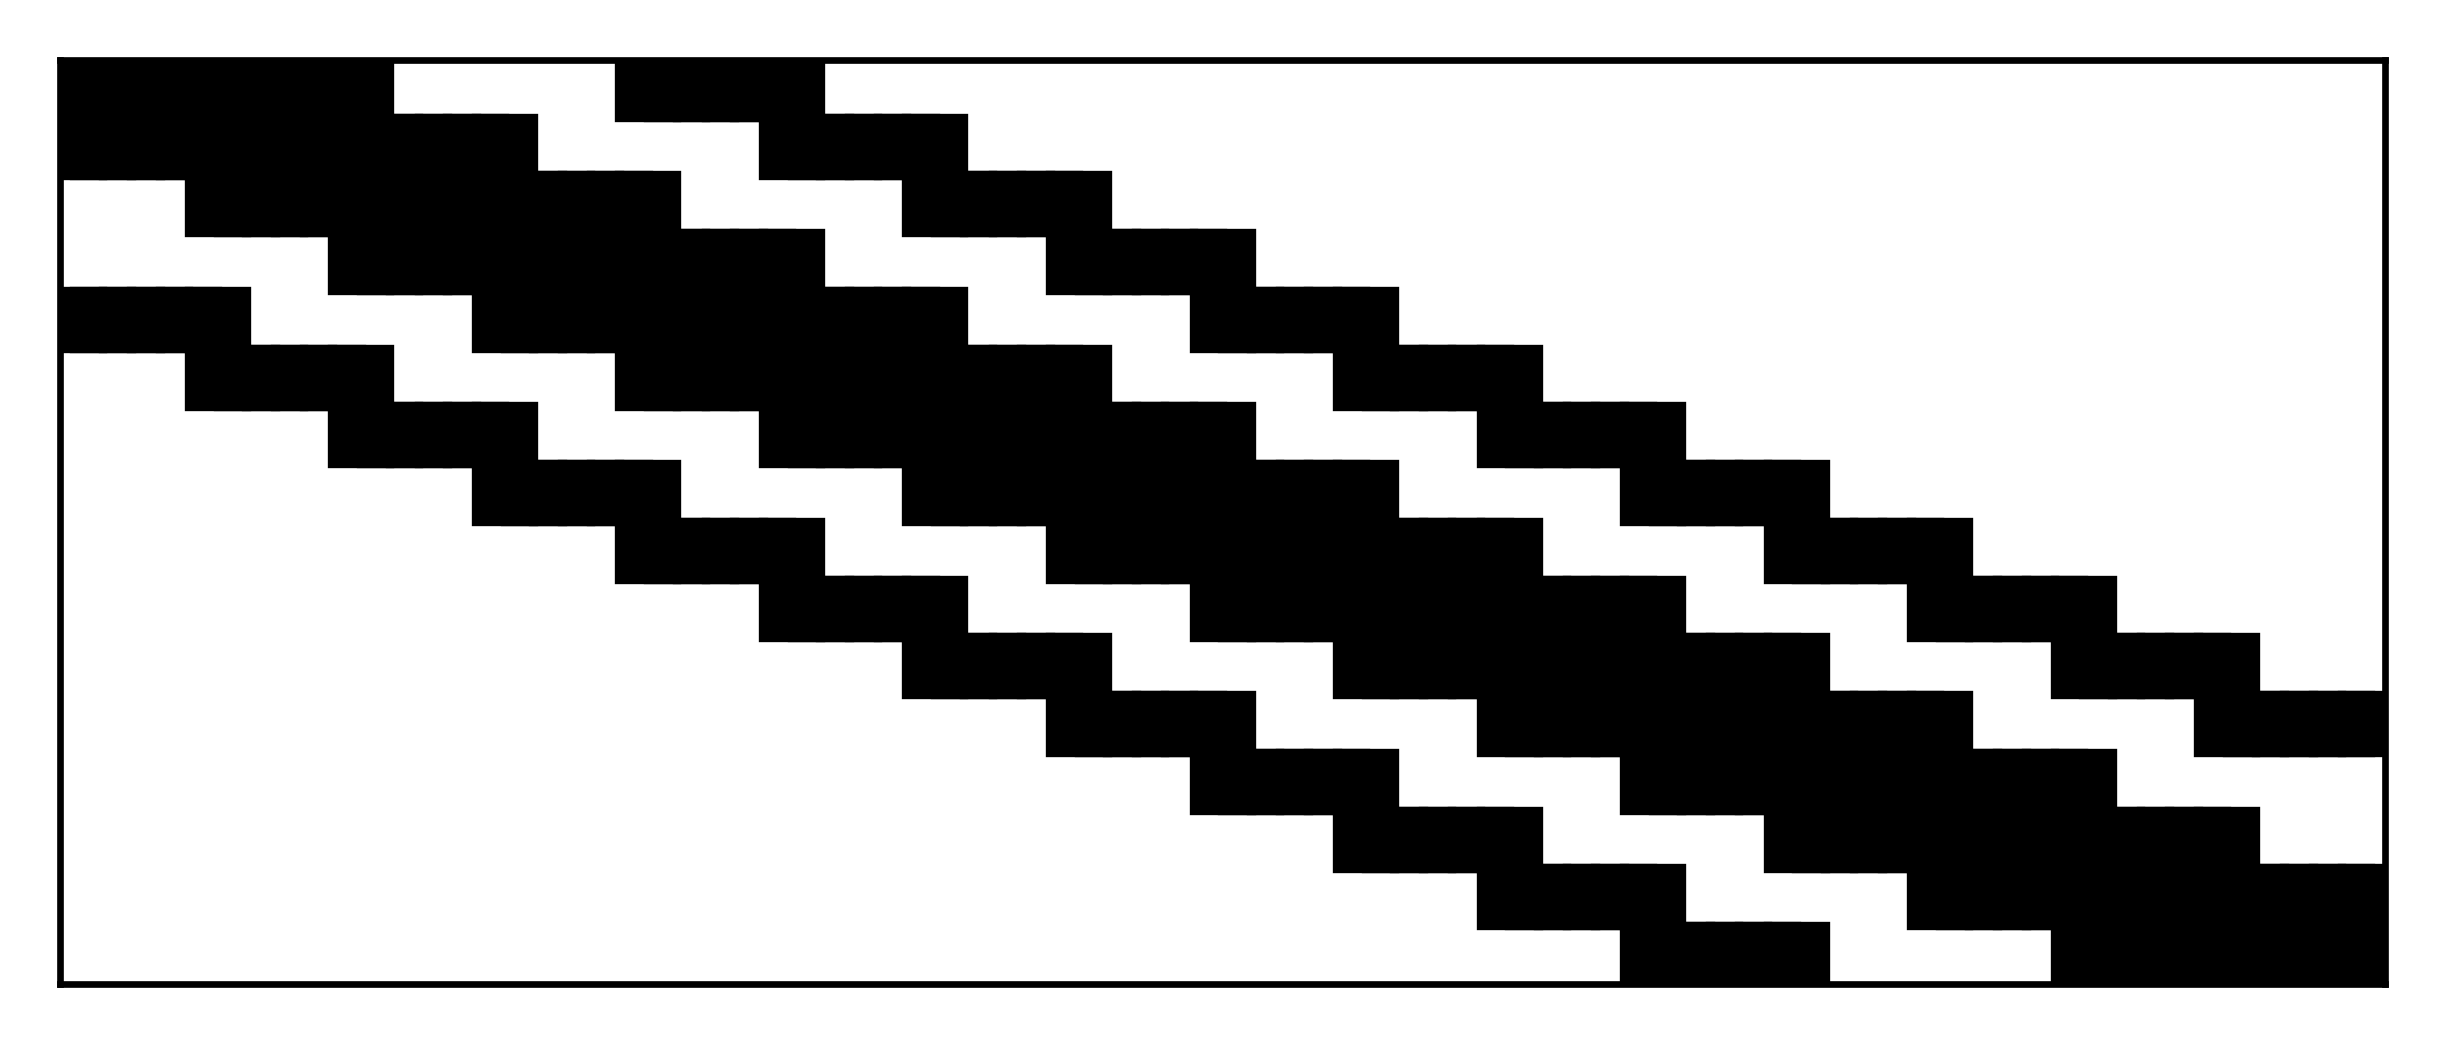
\includegraphics[width=\textwidth]{S.png}
        \end{center}
        \caption{$\btS$}
      \end{subfigure}
      \begin{subfigure}[b]{0.172\textwidth}
        \begin{center}
            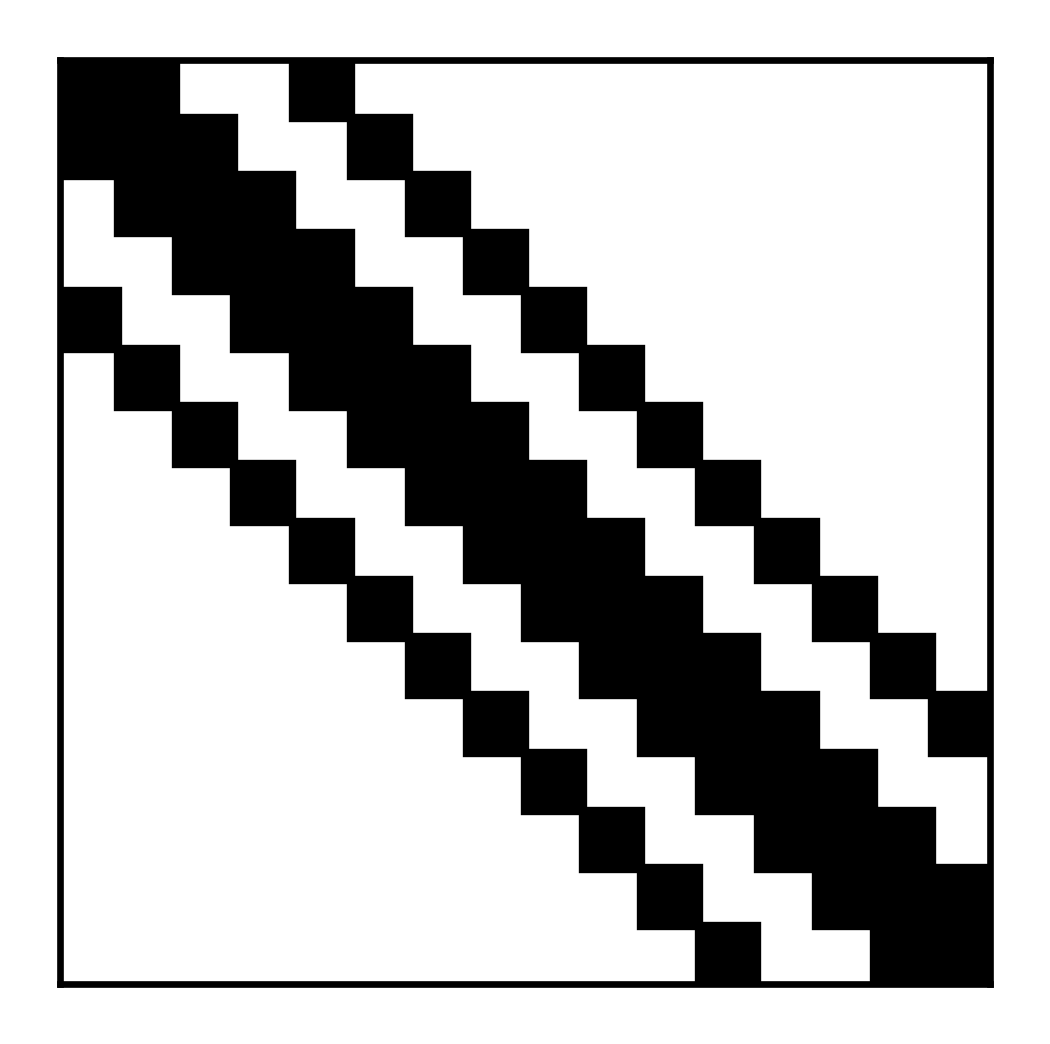
\includegraphics[width=\textwidth]{C.png}
        \end{center}
        \caption{$\btC$}
      \end{subfigure}
      \begin{subfigure}[b]{0.4\textwidth}
        \begin{center}
            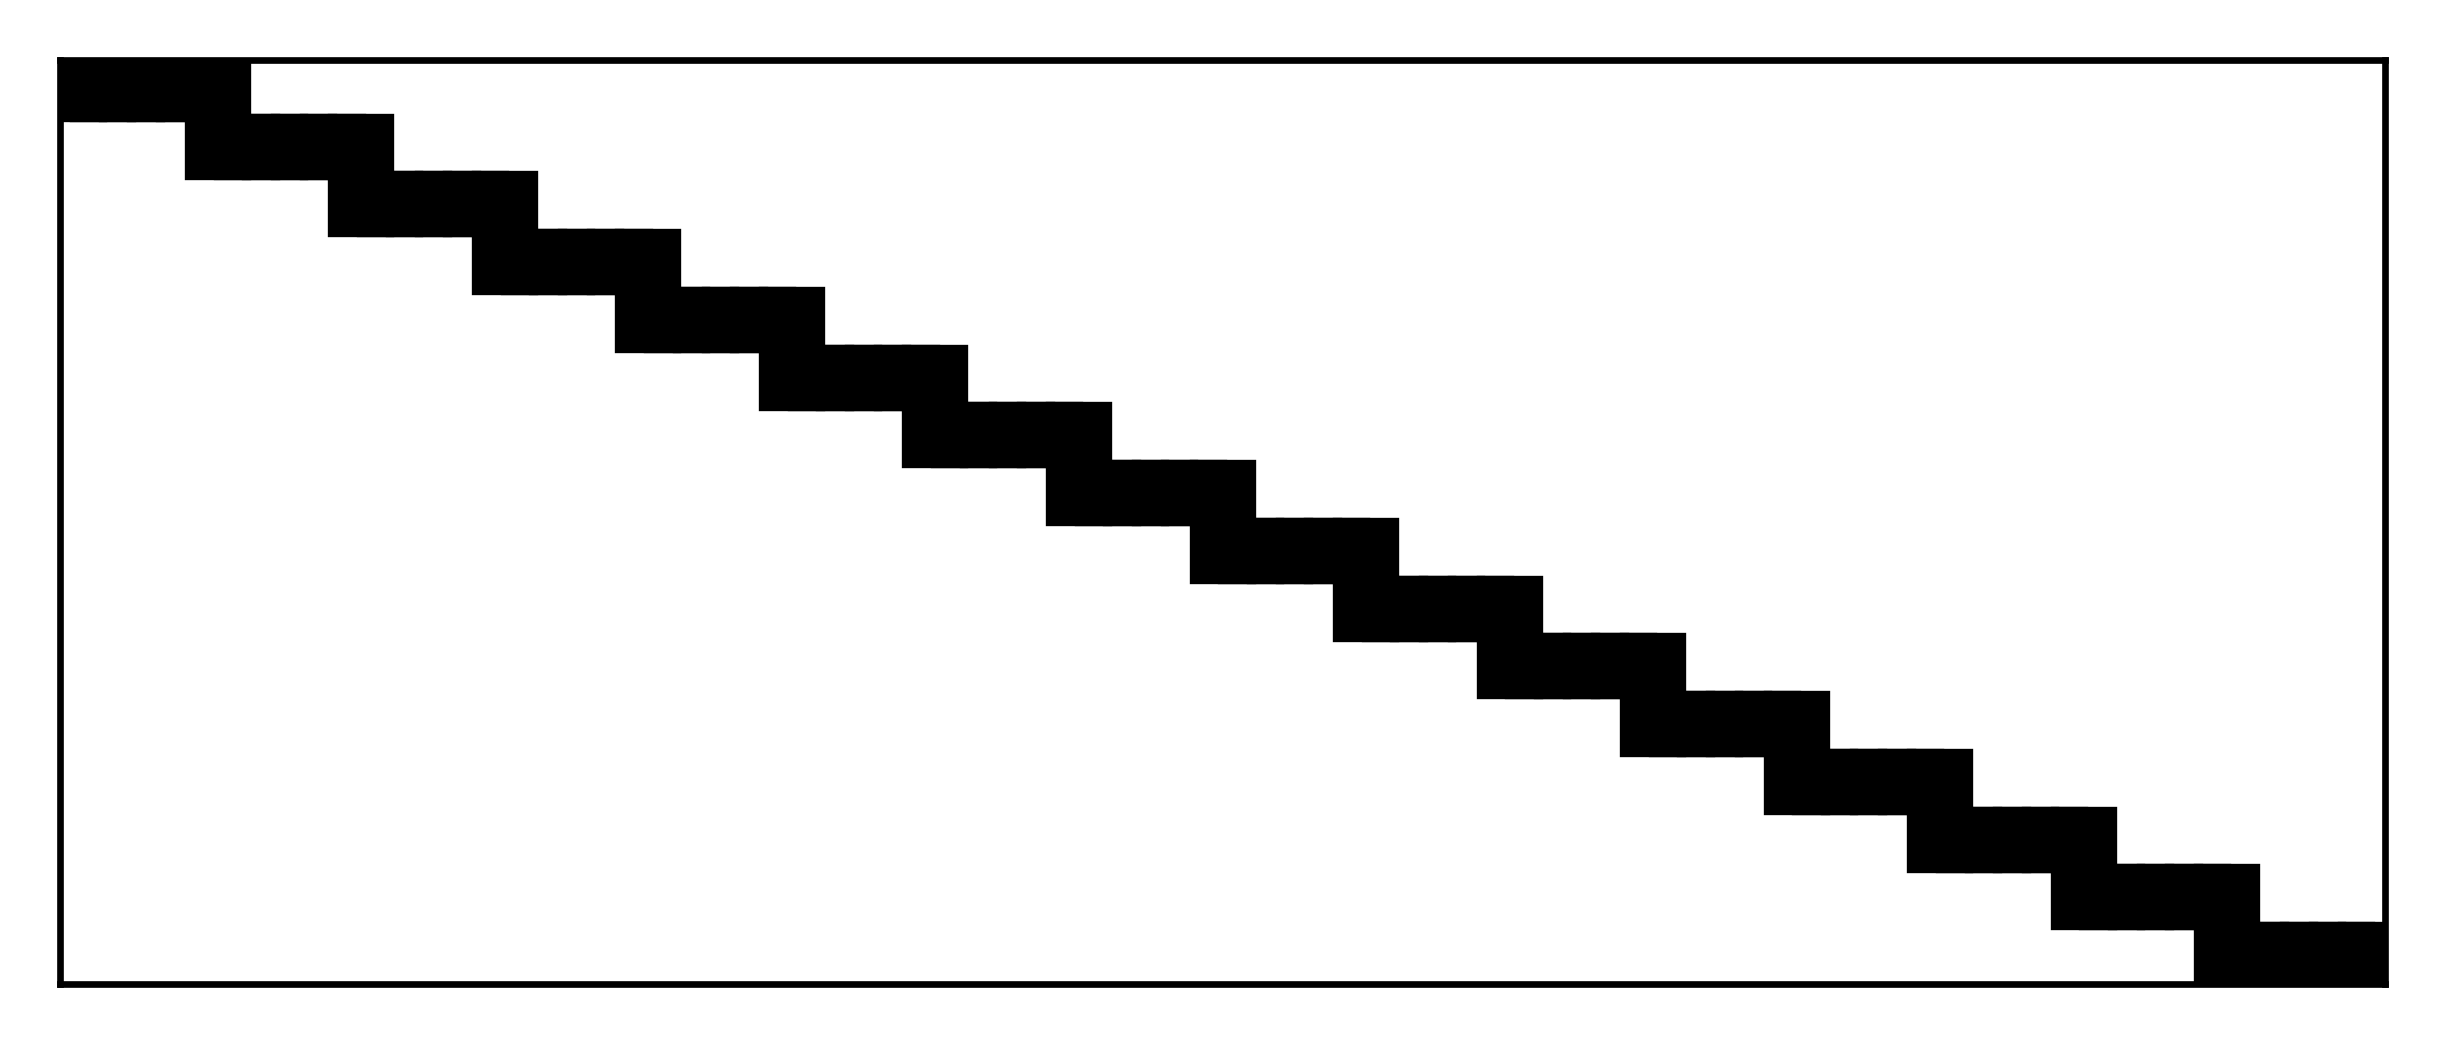
\includegraphics[width=\textwidth]{B.png}
        \end{center}
        \caption{$\btB$}
      \end{subfigure}
  \end{center}
  \caption[Mask matrix $\btS$, nodal connectivity matrix $\btC$, and base matrix $\btB$.]{Mask matrix $\btS$, nodal connectivity matrix $\btC$, and base matrix $\btB$ for $N = 16$, $M = 81$, $b = 6$, and $\delta b = 5$.}
  \label{fig: S,C,B}
\end{figure}

Following our convention, sparse autoencoders with or without activation functions in the encoder are denoted by NE-SAE and LE-SAE, respectively. 

\subsubsection{Convolutional Autoencoder with Enhanced Adaptivity}\label{sec: cnnae}

In this section, we propose to utilize Convolutional Neural Networks (CNNs) in the decoder to promote adaptivity. This choice is motivated by the fact that for PDEs with sharp solution gradients, the localization induced by convolutional filters helps extract local information from neighboring points, hence enabling high-quality reconstruction from the low-dimensional latent space $\mathcal{U}^r$. Our aim is to enhance adaptivity by considering trainable kernels in the convolution operator.

We define the decoder as
\begin{align} \label{eq: cnn decoder}
    D(\hat{\btu}^{\left<m\right>}) = \sum_{i=1}^r D_i(\hat{u}_i^{\left<m\right>}; \hat{\btu}^{\left<m\right>})\,,
\end{align}
where $D_i: \mathbb{R} \to \mathbb{R}^N$ is a lifting function defined as
\begin{align} \label{eq: cnn sub decoder}
    D_i(\hat{u}_i^{\left<m\right>}; \hat{\btu}^{\left<m\right>}) = (P \circ C_{\kappa_i}( \cdot\,; \hat{\btu}^{\left<m\right>}) \circ R \circ S_i)(\hat{u}_i^{\left<m\right>})\,,
\end{align}
where each term in the right-hand side is defined below.
\begin{itemize}
    \item The function $S_i$ is lifting $\hat{u}_i^{\left<m\right>}$ to a vector in $\mathbb{R}^N$ through the learnable mapping
    \begin{align}
    S_i(\hat{u}_i^{\left<m\right>}) = \btW_i \hat{u}_i^{\left<m\right>} + \btb_i\,,
    \end{align}
    where $\btW_i \in \mathbb{R}^N$ and $\btb_i \in \mathbb{R}^N$ are weights and bias of the fully connected layer.
    \item $R$ reshapes a vector in $\mathbb{R}^N$ into a matrix in $\mathbb{R}^{n_1 \times \ldots \times n_d}$, where $n_i$ specifies the number of degrees of freedom along the $i$th direction in the physical domain.
    \item The convolution function $C_{\kappa_i}:\mathbb{R}^{n_1 \times \ldots \times n_d} \to \mathbb{R}^{n_1 \times \ldots \times n_d}$ introduces adaptive spatial smoothing to capture localization. To define $C_{\kappa_i}$, we first introduce the kernel $\kappa_i:\mathbb{R}^r \to \mathbb{R}^{\mu^d}$ through the composite mapping
    \begin{align}
    \kappa_i = R_\kappa \circ ( K_i^{(n_k)} \circ K_i^{(n_k -1)} \circ ... \circ K_i^{(1)})\,,
    \end{align}
    where $K_i^{(n_k)} \circ K_i^{(n_k -1)} \circ ... \circ K_i^{(1)}$ is a neural network with $(n_k-1)$ hidden layers (with activation functions), i.e.,
    \begin{align}
    K_i^{(\ell)}(\btx) &= 
    \begin{cases} 
        \btW^{(\ell)}_i \btx + \btb^{(\ell)}_i\,, \quad \btW^{(\ell)}_i \in \mathbb{R}^{\mu^d \times q_{\ell - 1}}\,, \quad \btb^{(\ell)}_i \in \mathbb{R}^{\mu^d}\,,\quad \ell = n_k\,,\\
        a(\btW^{(\ell)}_i \btx + \btb^{(\ell)}_i)\,, \quad \btW^{(\ell)}_i \in \mathbb{R}^{p_\ell \times q_\ell} \,, \quad \btb^{(\ell)}_i \in \mathbb{R}^{p_\ell}\,, \quad \ell < n_k\,,
    \end{cases}
    \end{align}
    where $q_1 = r$ and the sets $\{p_\ell\}_{\ell = 1}^{n_k - 1}$ and $\{q_\ell\}_{\ell = 2}^{n_k - 1}$ are user-specified. The function $R_\kappa \in \mathbb{R}^{\mu^d} \mapsto \mathbb{R}^{\bigtimes_{j = 1}^d \mu}$ reshapes a vector into a matrix of size $\mu \times \ldots \times \mu $ ($d$ times). The function $C_{\kappa_i}$ then performs the discrete linear convolution of $(R \circ S_i)(\hat{u}_i^{\left<m\right>})$ with $\kappa_i(\hat{\btu}^{\left<m\right>})$.
    \item $P$ projects back from a matrix representation in $\mathbb{R}^{n_1 \times \ldots \times n_d}$ into a vector in $\mathbb{R}^N$.
\end{itemize}
In the above, and in contrast with strategies where the CNN is trained once for all, the trainable parameters in the kernel of the CNN are defined as the output of an auxiliary neural network and are, by construction, iteration-dependent: they evolve as a function of the latent solution vector to capture non-smoothness, hence promoting adaptivity.

The structure of the decoder $D$ is depicted in Fig.~\ref{fig: summary of cnnae}. 
\begin{figure}[!htb]
    \begin{center}
        \includegraphics[trim = {5.5cm 7cm 5.5cm 6.5cm}, clip, width = 0.8\linewidth]{FigSummaryCnnae.pdf}
    \end{center}
    \caption[General description of the CNN-based autoencoder.]{General description of the CNN-based autoencoder: $\btu^{\left<m\right>}$ is encoded into a latent vector $\hat{\btu}^{\left<m\right>}$ by the encoder. The latent vector is then decoded by the decoder to get $\tilde{\btu}^{\left<m\right>}$. A smoothing convolutional layer is added after the single dense layer at the beginning of the decoder to introduce nonlinearity into the decoder.}
    \label{fig: summary of cnnae}
\end{figure}
This convolutional autoencoder (denoted by CNNAE, with the LE-CNNAE and NE-CNNAE variations depending on whether activation functions are used in the encoder) is also trained by minimizing the mean squared loss given by Eq.~\eqref{eq: mse}.

\subsection{Strategies for Operator Learning Between Latent Spaces}\label{sec: operators}

We now turn to the construction of the surrogate operator $\mathcal{H}: \mathcal{U}_0^r \to \mathcal{U}^r$ mapping $\hat{\btu}_0 = E(u_0)$ to $\hat{\btu} = E(\btu)$. To this end, we consider the reduced-order model
\begin{equation}
    \frac{\partial \hat{\btu}(t)}{\partial t} = F(\hat{\btu}(t))\,, \quad \hat{\btu}(0) = \hat{\btu}_0\,,
\end{equation}
where the operator $F$ in the right-hand side is learned through an \textit{ad hoc} technique. We restrict the discussion below to two classes of techniques. The first class involves so-called quadratic operator inference \cite{qian2022reduced}, which is an efficient operator learning method that does not necessitate the definition and training of a deep learning model. This approach is briefly introduced in Section \ref{sec: opinf}. The second approach involves a simple feedforward neural network model, detailed in Section \ref{sec: dnnop}. Regarding time integration, we rely on the implicit backward Euler method, combined with a standard Newton-Raphson solver. 

\subsubsection{Quadratic Operator Inference}\label{sec: opinf}
Following \cite{qian2022reduced}, the operator inference (OpInf) approach approximates a reduced operator of the polynomial form (with linear and quadratic reduced operators). It then casts PDEs with more general nonlinear terms through the use of lifting variable transformations which expose quadratic structure in the PDE.

OpInf seeks a linear operator $\btA$ and a quadratic operator $\btH$ by minimizing the approximation error in the least-squares sense
\begin{align}
    \min_{\btA\in\mathbb{R}^{r \times r}\,,~ \btH\in\mathbb{R}^{r \times r^2}} \dfrac{1}{N_{snp}} \sum_{\ell = 1}^{N_{ic}} \sum_{m = 0}^{N_t} \norm{\btA \hat{\btu}^{\left<m\right>}(u_0^{(\ell)}) + \btH\left( \hat{\btu}^{\left<m\right>}(u_0^{(\ell)}) \otimes \hat{\btu}^{\left<m\right>}(u_0^{(\ell)})\right) - \dot{\hat{\btu}}^{\left<m\right>}(u_0^{(\ell)})}^2\,,\label{eq: opinf least squares}
\end{align}
with the corresponding matrix algebraic form
\begin{align}
    &\btD
    \begin{bmatrix}
        \btA^T\\
        \btH^T
    \end{bmatrix} = \dot{\hat{\btU}}\,,\label{eq:opinf}
\end{align}
where the least-squares data matrix $D \in \mathbb{R}^{r \times (r + r^2)}$ and the right-hand side $\dot{\hat{\btU}} \in \mathbb{R}^{r \times N_{snp}}$ are given by
\begin{align}
    \btD = 
    \begin{bmatrix}
        \hat{\btu}^{\left<0\right>}(u_0^{(1)})& \ldots & \hat{\btu}^{\left<N_t\right>}(u_0^{(1)}) & \ldots & \hat{\btu}^{\left<N_t\right>}(u_0^{(N_{ic})})\\
        \hat{\btu}^{\left<0\right>}(u_0^{(1)}) \otimes \hat{\btu}^{\left<0\right>}(u_0^{(1)}) & \ldots & \hat{\btu}^{\left<N_t\right>}(u_0^{(1)}) \otimes \hat{\btu}^{\left<N_t\right>}(u_0^{(1)}) & \ldots & \hat{\btu}^{\left<N_t\right>}(u_0^{(N_{ic})}) \otimes \hat{\btu}^{\left<N_t\right>}(u_0^{(N_{ic})})
    \end{bmatrix}^T
\end{align}
and
\begin{align}
    \dot{\hat{\btU}} = \begin{bmatrix} \dot{\hat{\btu}}^{\left<0\right>}(u_0^{(1)}) & \ldots & \dot{\hat{\btu}}^{\left<N_t\right>}(u_0^{(1)}) & \ldots & \dot{\hat{\btu}}^{\left<N_t\right>}(u_0^{(N_{ic})})
    \end{bmatrix}\,,
\end{align}
respectively. The reduced operator is then given by
\begin{align}
    F(\hat{\btu}^{\left<m\right>}) = \btA\hat{\btu}^{\left<m\right>} + \btH \left(\hat{\btu}^{\left<m\right>} \otimes \hat{\btu}^{\left<m\right>}\right)\,.
\end{align}
The combination of the above operator with the time integration scheme defines the surrogate operator $\mathcal{H}$.

\subsubsection{Deep Neural Network-Based Operator}\label{sec: dnnop}

In addition to the above OpInf framework, we also explore the use of a simple deep neural network to approximate the reduced operator $F$. The DNN-based operator (DNNOp) is defined as
\begin{align}\label{eq:DNNOp-over}
    F(\hat{\btu}^{\left<m\right>}) = O(\hat{\btu}^{\left<m\right>}),
\end{align}
where $O:\mathbb{R}^r \to \mathbb{R}^r$ is a deep neural network
    \begin{align}
    O =  O^{(n_o)} \circ O^{(n_o -1)} \circ ... \circ O^{(1)}\,,
    \end{align}
    with $(n_o-1)$ hidden layers (with activation functions), i.e.,
    \begin{align}
    O^{(\ell)}(\btx) &= 
    \begin{cases} 
        \btW^{(\ell)} \btx + \btb^{(\ell)}\,, \quad \btW^{(\ell)} \in \mathbb{R}^{r \times q_{\ell - 1}}\,, \quad \btb^{(\ell)} \in \mathbb{R}^r\,,\quad \ell = n_o\,,\\
        a(\btW^{(\ell)} \btx + \btb^{(\ell)})\,, \quad \btW^{(\ell)} \in \mathbb{R}^{p_\ell \times q_\ell} \,, \quad \btb^{(\ell)}_i \in \mathbb{R}^{p_\ell}\,, \quad \ell < n_o\,,
    \end{cases}
    \end{align}
    with $q_1 = r$. The dimensions in the hidden layers $\{p_\ell\}_{\ell = 1}^{n_k - 1}$ and $\{q_\ell\}_{\ell = 2}^{n_k - 1}$ are chosen while devising the architecture.
    
The operator is trained by minimizing the projection error defined as
\begin{align}
    l^{\text{proj}}_{\text{DNNOp}}(\hat{\btU}; \boldsymbol{\Theta}_o) = \frac{\sqrt{\sum_{l=1}^{N_{ic}}\sum_{m=0}^{N_t}\norm{\dot{\hat{\btu}}^{\left<m\right>}(u_0^{(\ell)}) - \rtO(\hat{\btu}^{\left<m\right>}(u_0^{(\ell)}); \boldsymbol{\Theta}_o)}^2}}{\sqrt{\sum_{l=1}^{N_{ic}}\sum_{m=0}^{N_t}\norm{\dot{\hat{\btu}}^{\left<m\right>}(u_0^{(\ell)})}^2}}\,,
\end{align}
where $\boldsymbol{\Theta}_o$ contains all trainable parameters in the reduced operator. The use of the approximation in Eq.~\eqref{eq:DNNOp-over} with the time integrator defines the DNNOp variant for $\mathcal{H}$.

\section{Vectorized Implicit Time Integration}

Ultimately, the surrogate of the flow map operator is applied to find solutions to the FOM at various times with different initial conditions. To that end, numerical time integration methods are used. Many of the physical systems with sharp gradients (such as the Burger's equation considered in this work) are ``stiff'' and numerically unstable. If an explicit time integration method is used, a prohibitively small time step size is often required to obtain an accurate solution. Furthermore, due to intrinsic dependence on time step size (as illustrated in Section \ref{subsec:time-dependency}), the same time step sizes used in the offline training phase are preferred. Given these considerations, all online evaluations in this work are performed using the implicit backward Euler time integration.

On the other hand, since General-Purpose Graphics Processing Unit (GPGPU)-enabled computing devices are used in the offline training process, it is preferable to take advantage of the hardware acceleration also in the online evaluation phase. However, a conundrum arises: 
\begin{itemize}
    \item The discretized surrogate of the map operator is by definition \emph{small}, i.e. the solution vector in the latent space is of size $r \ll N$, and the linearized system is of size $r \times r$, and the solution at time step $m$ depends on the solution from $m-1$.
    \item Modern GPGPU-enabled computing devices rely on being able to handle a \emph{large} amount of workload in a vectorized fashion. 
\end{itemize}
In other words, the effective and accurate surrogate operator will unfortunately starve the computing device for work. To address this issue, we propose a new technique to effectively ``vectorize'' the time integration in parallel, in order to increase the workload, i.e. from a system of size $r \times r$ to a system of size $m_c \times r \times r$, where $m_c \leq m$ is the number of ``chunked'' time steps to be explained momentarily. The basic idea/algorithm is to assemble $m_c$ linearized systems in a vectorized fashion, form an implicit system of size $m_c n \times m_c n$, and then solve the system of equations again in a vectorized fashion by exploiting its special block-bidiagonal structure. Each step of the algorithm is described in the following paragraphs.

\paragraph{Increasing the size of the linearized system}
Consider a ``chunk'' of $m_c$ time steps integrating the surrogate flow map from time $t_i$ to time $t_{i+m_c}$.  Recast the solution at each of these time steps in an incremental form as
\begin{equation}
    \hat{\btu}_{i+j} = \hat{\btu}_{i} + \Delta \hat{\btu}_j.
\end{equation}
That is, the solution $\hat{\btu}_{i+j}$ at a given time is equal to the solution $\hat{\btu}_i$ at the start of the chunk of time steps plus an increment $\Delta \hat{\btu}_j$.  With this rearrangement, we can write the implicit time integration equations for the entire chunk of $m_c$ steps as
\begin{equation}
    \begin{bmatrix}
    F\left(\hat{\btu}_{i}, \hat{\btu}_{i} + \Delta \hat{\btu}_{1}, t_{i+1}, t_{i}\right)\\ 
    F\left(\hat{\btu}_{i}+ \Delta \hat{\btu}_{1}, \hat{\btu}_{i} + \Delta \hat{\btu}_{2}, t_{i+2}, t_{i+1}\right)\\ 
    \vdots\\ 
    F\left(\hat{\btu}_{i} + \Delta \hat{\btu}_{j}, \hat{\btu}_{i} + \Delta \hat{\btu}_{j-1}, t_{i+j}, t_{i+j-1}\right)
    \end{bmatrix} = \boldsymbol{0}.
\end{equation}
Or, specifically for the backward Euler scheme\footnote{The algorithm is derived based on the backward Euler scheme but can be trivially generalized to other (higher order) variants.}:
\begin{equation}
    \begin{bmatrix}
    \Delta \hat{\btu}_{1} - h\left(\hat{\btu}_{i} + \Delta \hat{\btu}_{1}, t_{i+1}; p \right) \Delta t_{i+1}\\ 
    \Delta \hat{\btu}_{2} - \Delta \hat{\btu}_{1} - h\left(\hat{\btu}_{i} + \Delta \hat{\btu}_{2}, t_{i+2}; p \right) \Delta t_{i+2}\\ 
    \vdots\\ 
    \Delta \hat{\btu}_{j} - \Delta \hat{\btu}_{j-1} - h\left(\hat{\btu}_{i} + \Delta \hat{\btu}_{j}, t_{i+j}; p \right) \Delta t_{i+j}
    \end{bmatrix} = \boldsymbol{0}.
    \label{eq:batched-backward-euler}
\end{equation}
In the simple, serial time integration scheme the nonlinear system has dimension $r$.  The nonlinear system for this vectorized time integration scheme (Eq.~\ref{eq:batched-backward-euler}) has dimension $m_c \times r$.  Clearly this approach can fully consume the available bandwidth of the computing device with a sufficiently large $m_c$. Equation \ref{eq:batched-backward-euler} is still nonlinear.  Applying the Newton-Raphson method provides the update algorithm
\begin{equation}
    \begin{split}
    \begin{bmatrix}
    \prescript{}{k+1} \Delta \hat{\btu}_{1}\\ 
    \prescript{}{k+1} \Delta \hat{\btu}_{2}\\ 
    \vdots\\ 
    \prescript{}{k+1} \Delta \hat{\btu}_{j}
    \end{bmatrix} = & \begin{bmatrix}
    \prescript{}{k} \Delta \hat{\btu}_{1}\\ 
    \prescript{}{k} \Delta \hat{\btu}_{2}\\ 
    \vdots\\ 
    \prescript{}{k} \Delta \hat{\btu}_{j}
    \end{bmatrix} - \prescript{}{k}{J}_{i+1}^{-1} \begin{bmatrix}
    \prescript{}{k} \Delta \hat{\btu}_{1} - h\left(\hat{\btu}_{i} + \prescript{}{k} \Delta \hat{\btu}_{1}, t_{i+1}; p \right) \Delta t_{i+1}\\ 
    \prescript{}{k} \Delta \hat{\btu}_{2} - \prescript{}{k} \Delta \hat{\btu}_{1} - h\left(\hat{\btu}_{i} + \prescript{}{k} \Delta \hat{\btu}_{2}, t_{i+2}; p \right) \Delta t_{i+2}\\ 
    \vdots\\ 
    \prescript{}{k} \Delta \hat{\btu}_{j} - \prescript{}{k} \Delta \hat{\btu}_{j-1} - h\left(\hat{\btu}_{i} + \prescript{}{k} \Delta \hat{\btu}_{j}, t_{i+j}; p \right) \Delta t_{i+j}
    \end{bmatrix}
    \end{split}
    \label{eq:batched-update}
\end{equation}
where the chunked discrete Jacobian has a bidiagonal form
\begin{equation}
    \prescript{}{k}{J}_{i+1} = \begin{bmatrix}
I - \prescript{}{k}J_{i+1}^\dagger & 0  & \cdots & 0 & 0 \\ 
-I & I - \prescript{}{k}J_{i+2}^\dagger  & 0  & \cdots & 0 \\ 
0 & -I & I - \prescript{}{k}J_{i+3}^\dagger  & \cdots  & 0 \\ 
\vdots  & \vdots  & \ddots & \ddots  & \vdots \\
0 & 0 & 0  & -I &  I - \prescript{}{k}J_{i+j}^\dagger
\end{bmatrix}
\end{equation}
where $\prescript{}{k}J_{i+j}^\dagger$ is the ODE Jacobian evaluated at the current values of the state $\hat{\btu}_i + \prescript{}{k}\Delta \hat{\btu}_{j}$, and $I$ is the identity matrix. The key linear algebra kernel for the vectorized time integration is solving potentially batched, block-bidiagonal\footnote{We note that the system is lower-block-bidiagonal. However, in the case of integrating the surrogate flow operator ``backward'' in time for solving an adjoint problem, the system is upper-block-bidiagonal. Both Thomas's algorithm and PCR work in these two cases.} systems of this type (Eq.~\ref{eq:block-bidiagonal}) to update the current Newton-Raphson iterate for the incremental solution.  The following two paragraphs discuss two viable algorithms, namely Thomas's algorithm and parallel cyclic reduction (PCR), to efficiently solve systems of this type.
\begin{equation}
\begin{bmatrix}
A_1 &  &  &  & \\ 
B_1 & A_2 &  &  & \\ 
 & B_2 & A_3 &  & \\ 
 &  & \ddots & \ddots & \\ 
 &  &  & B_{n-1} & A_n
\end{bmatrix} \begin{bmatrix}
x_1\\ 
x_2\\ 
x_3\\ 
\vdots\\ 
x_n
\end{bmatrix} = \begin{bmatrix}
y_1\\ 
y_2\\ 
y_3\\ 
\vdots\\ 
y_n
\end{bmatrix}
\label{eq:block-bidiagonal}
\end{equation}

\paragraph{Thomas algorithm}
The Thomas algorithm sweeps down the diagonal blocks of the matrix, solving for each block of unknown solution $\hat{\btu}_i$ one-by-one.  Algorithm \ref{alg:thomas} summarizes the process.  All the matrix operations in this algorithm can be batched over an additional batch dimension, e.g. for different initial conditions.

\begin{algorithm}
\caption{Thomas algorithm for solving batched, block-bidiagonal matrix systems.}\label{alg:thomas}
\begin{algorithmic}
\State $x_1 = A_{1}^{-1} y_1$
\State $i \gets 1$
\While{$i < m_c$}
\State $x_{i+1} \gets A_{i+1}^{-1} \left(y_{i+1} - B_{i} x_{i} \right)$
\State $i \gets i + 1$
\EndWhile
\end{algorithmic}
\end{algorithm}

\paragraph{Parallel cyclic reduction (PCR)}
Parallel cyclic reduction is a divide-and-conquer algorithm that recursively splits a (batched, blocked) bidiagonal matrix into two independent bidiagonal linear systems.  The following equations give the basic update, splitting a single bidiagonal system 
\begin{equation}
\begin{bmatrix}
A_1 & 0 & 0 & 0\\ 
B_1 & A_2 & 0 & 0\\ 
0 & B_2 & A_3 & 0\\ 
0 & 0 & B_3 & A_4
\end{bmatrix} \begin{bmatrix}
x_1\\ 
x_2\\ 
x_3\\ 
x_4
\end{bmatrix} = \begin{bmatrix}
y_1\\ 
y_2\\ 
y_3\\ 
y_4
\end{bmatrix}
\end{equation}
into two independent bidiagonal systems
\begin{equation}
\begin{bmatrix}
A_1 & 0 & 0 & 0\\ 
0 & A_2 & 0 & 0\\ 
-B_2 A_2^{-1} B_1 & 0 & A_3 & 0\\ 
0 & -B_3 A_3^{-1} B_2 & 0 & A_4
\end{bmatrix} \begin{bmatrix}
x_1\\ 
x_2\\ 
x_3\\ 
x_4
\end{bmatrix} = \begin{bmatrix}
y_1\\ 
y_2 - B_1 A_1^{-1} y_1\\ 
y_3 - B_2 A_2^{-1} y_2\\ 
y_4 - B_3 A_3^{-1} y_3
\end{bmatrix}
\end{equation}
where the first subsystem corresponds to $(x_1, x_3)$, and the second subsystem corresponds to $(x_2, x_4)$. PCR then recursively applies this splitting formula to further subdivide the matrices until it reaches a block diagonal form.  Algorithm \ref{alg:pcr} describes the complete process.  The key point in PCR is that the new matrices produced by each application of the splitting formula can be factored independently, in parallel.

\begin{algorithm}
\caption{Parallel cyclic reduction algorithm for solving batched, block-bidiagonal matrix systems.}\label{alg:pcr}
\begin{algorithmic}
\State $i \gets 1$
\While{$i<\log_2{m_c}$}
\State Form $2^i$ submatrices by taking every $2^i$th row
\For{submatrix $j=1$ to $j=2^i$} \Comment{This loop can be vectorized}
\For{index $k\in$ submatrix $j$}
\State $B_k \gets -B_k D_k^{-1}B_{k-1}$
\State $y_k \gets y_k - B_k D_{k-1}^{-1} y_{k-1}$
\EndFor
\EndFor
\State $i \gets i + 1$
\EndWhile \\
\Return $x \gets y$
\end{algorithmic}
\end{algorithm}

\begin{remark}
Naturally, a third option could be to start solving the system with PCR, but halt the recursive subdivision before reducing the system to a series of diagonal blocks and instead solve the remaining, unreduced sets of independent equations using Thomas algorithm.  This approach has an extra parameter controlling the heuristic, the number of iterations after which to switch from PCR to Thomas, $\bar{m}$.
\end{remark}

\paragraph{Time complexities of vectorized time integration algorithms}
Without considering parallelization and vectorization over the batched matrix operations, the Thomas algorithm is serial with time complexity $O(m_c r^3)$, including the cost of back propagation loop and the cost of factorizing the diagonal blocks. Note this is considerably cheaper than solving the full dense matrix, which would be $O(m_c^3 r^3)$. PCR, on the other hand, has time complexity $O(\log_2(m_c) m_c r^3 + m_c r^3)$. However, if the computing device can accommodate the full amount of available parallel work ($m_c$ submatrices on the final iteration), which is a reasonable assumption for a GPU and the size of the discretized flow map surrogate, the time complexity becomes $O(m_c r^3)$. The two algorithms therefore have the same asymptotic performance dominated by the cost of factorizing the diagonal blocks, assuming perfect vectorization of PCR.  However, in practice, as explored in the timing studies, the two algorithms are competitive depending on the size of the system (defined by $m_c$ and $r$, as suggested by the differing complexity of the reduction/back-propagation part of the analysis).

\section{Application to 2D Burgers' Equation}\label{sec:example}
\subsection{Description of the Problem}
Consider the parameterized 2D viscous Burgers' equation
\begin{subequations}
    \begin{align}
       \frac{\partial u}{\partial t} + u \frac{\partial u}{\partial x} + v \frac{\partial u}{\partial y} = \frac{1}{\mathrm{Re}}\left( \frac{\partial^2 u}{\partial x^2} + \frac{\partial^2 u}{\partial y^2} \right)\,, \\
       \frac{\partial v}{\partial t} + u \frac{\partial v}{\partial x} + v \frac{\partial v}{\partial y} = \frac{1}{\mathrm{Re}}\left( \frac{\partial^2 v}{\partial x^2} + \frac{\partial^2 v}{\partial y^2} \right), \\ (x, y) \in \Omega = [0,1] \times [0, 1], \quad t \in [0, 2]\,,
    \end{align}
\end{subequations}
where $u, v: \Omega \times T \mapsto \mathbb{R}$ are scalar-valued time-dependent velocities in the $x$ and $y$ directions, respectively, and $\mathrm{Re}$ is the Reynolds number. In this work, we consider $\mathrm{Re} = 10000$ to enforce sharp gradients in the solution. We note that standard values used to benchmark learning methods are in the range $\mathrm{Re} \in [10, 5000]$, with a larger representation of low Reynolds numbers (e.g., $\mathrm{Re} = 100$ in \cite{LU2022114778,kovachki2023neural}). The initial conditions are given as
\begin{subequations}
    \begin{align}
        u(x,y,0;\mu) &= \begin{cases}
                \mu \sin(2 \pi x) \sin(2 \pi y)\,, & \text{if } (x, y) \in [0,0.5] \times [0,0.5]\,,\\
                0\,, & \text{otherwise}\,,
            \end{cases} \\
        v(x,y,0;\mu) &= \begin{cases}
                \mu \sin(2 \pi x) \sin(2 \pi y)\,, & \text{if } (x, y) \in [0,0.5] \times [0,0.5]\,,\\
                0\,, & \text{otherwise}\,,
            \end{cases}
    \end{align}
\end{subequations}
with zero boundary conditions on the edges. The spatial domain $\Omega$ is discretized into $(n_x-1)$ and $(n_y-1)$ uniform meshes with linear quadrilateral elements in $x$ and $y$ directions, respectively, with $n_x = 60$, $n_y = 60$. The number of uniform time steps $n_t = 1500$. 

To enable fair comparison and reproducibility, the solution snapshots used by the authors in \cite{kim2022fast} were used for $\mu = \{0.9, 0.95, 1.05, 1.1\}$.  A separate dataset obtained with $\mu = 1.0$ was used for testing the generalization ability of the models (test dataset).

\subsection{Training of Autoencoders}

Autoencoders are trained using $90\%$ of the reference solution from the training dataset, while the remaining $10\%$ data points are considered as the validation dataset. The test dataset is not used during the offline training process and is used for performance comparison between all autoencoders and reduced operators.

For the deep autoencoders (LE-DAE and NE-DAE), we use a hidden layer of size $M_1 = 6728$ in the encoder, and a hidden layer of size $M_2 = 33730$ in the decoder. For the sparse autoencoders (LE-SAE and NE-SAE), we use the same neural network structure with the shallow mask built as shown in \eqref{eq: shallow mask}, with bandwidth $b = 70$, and shift $\delta = \lfloor (M - b) / (N - 1) \rfloor = 10$. For the convolutional autoencoders (LE-CNNAE and NE-CNNAE), we use one hidden layer of size $M_e = 200$ in the encoder, and the nonlinear mapping for the smoothing kernels are obtained by a deep neural network with one hidden layer of size $M_{\mu} = 200$, with the size of the kernel $\mu = 5$. We use the whole training dataset to learn the bases of the POD, and evaluate it on the test dataset as well.

For the training strategies, we employ the Adam optimizer \cite{kingma2014adam}, which is a variant of stochastic gradient descent (SGD), with an initial learning rate set to $0.001$. For the deep and sparse autoencoders, we split the training dataset into $n_{\text{batch}} = 22$ batches, and use maximum patience of 100 epochs such that the learning rate will decrease by a factor of 10 when a training loss stagnates for 100 successive training epochs. For the convolutional autoencoders, we split the training dataset into $n_{\text{batch}} = 240$ batches and use maximum patience of 100 epochs as well. We experimented model training with different batch sizes, and choose different batch sizes for the deep/sparse autoencoder and the convolutional based autoencoder based on best performances. We consider four different latent space dimensions: $r \in \{ 5, 10, 15, 20 \}$. The train and validation loss (mean-squared error) histories for all autoencoders with $r = 20$ are shown in Fig.~\ref{fig: train test history}. The training and validation losses are fairly close to each other showing good balance between accuracy and overfitting.
\begin{figure}[!htb]
     \begin{center}
        \begin{subfigure}[b]{0.49\textwidth}
            \begin{center}
                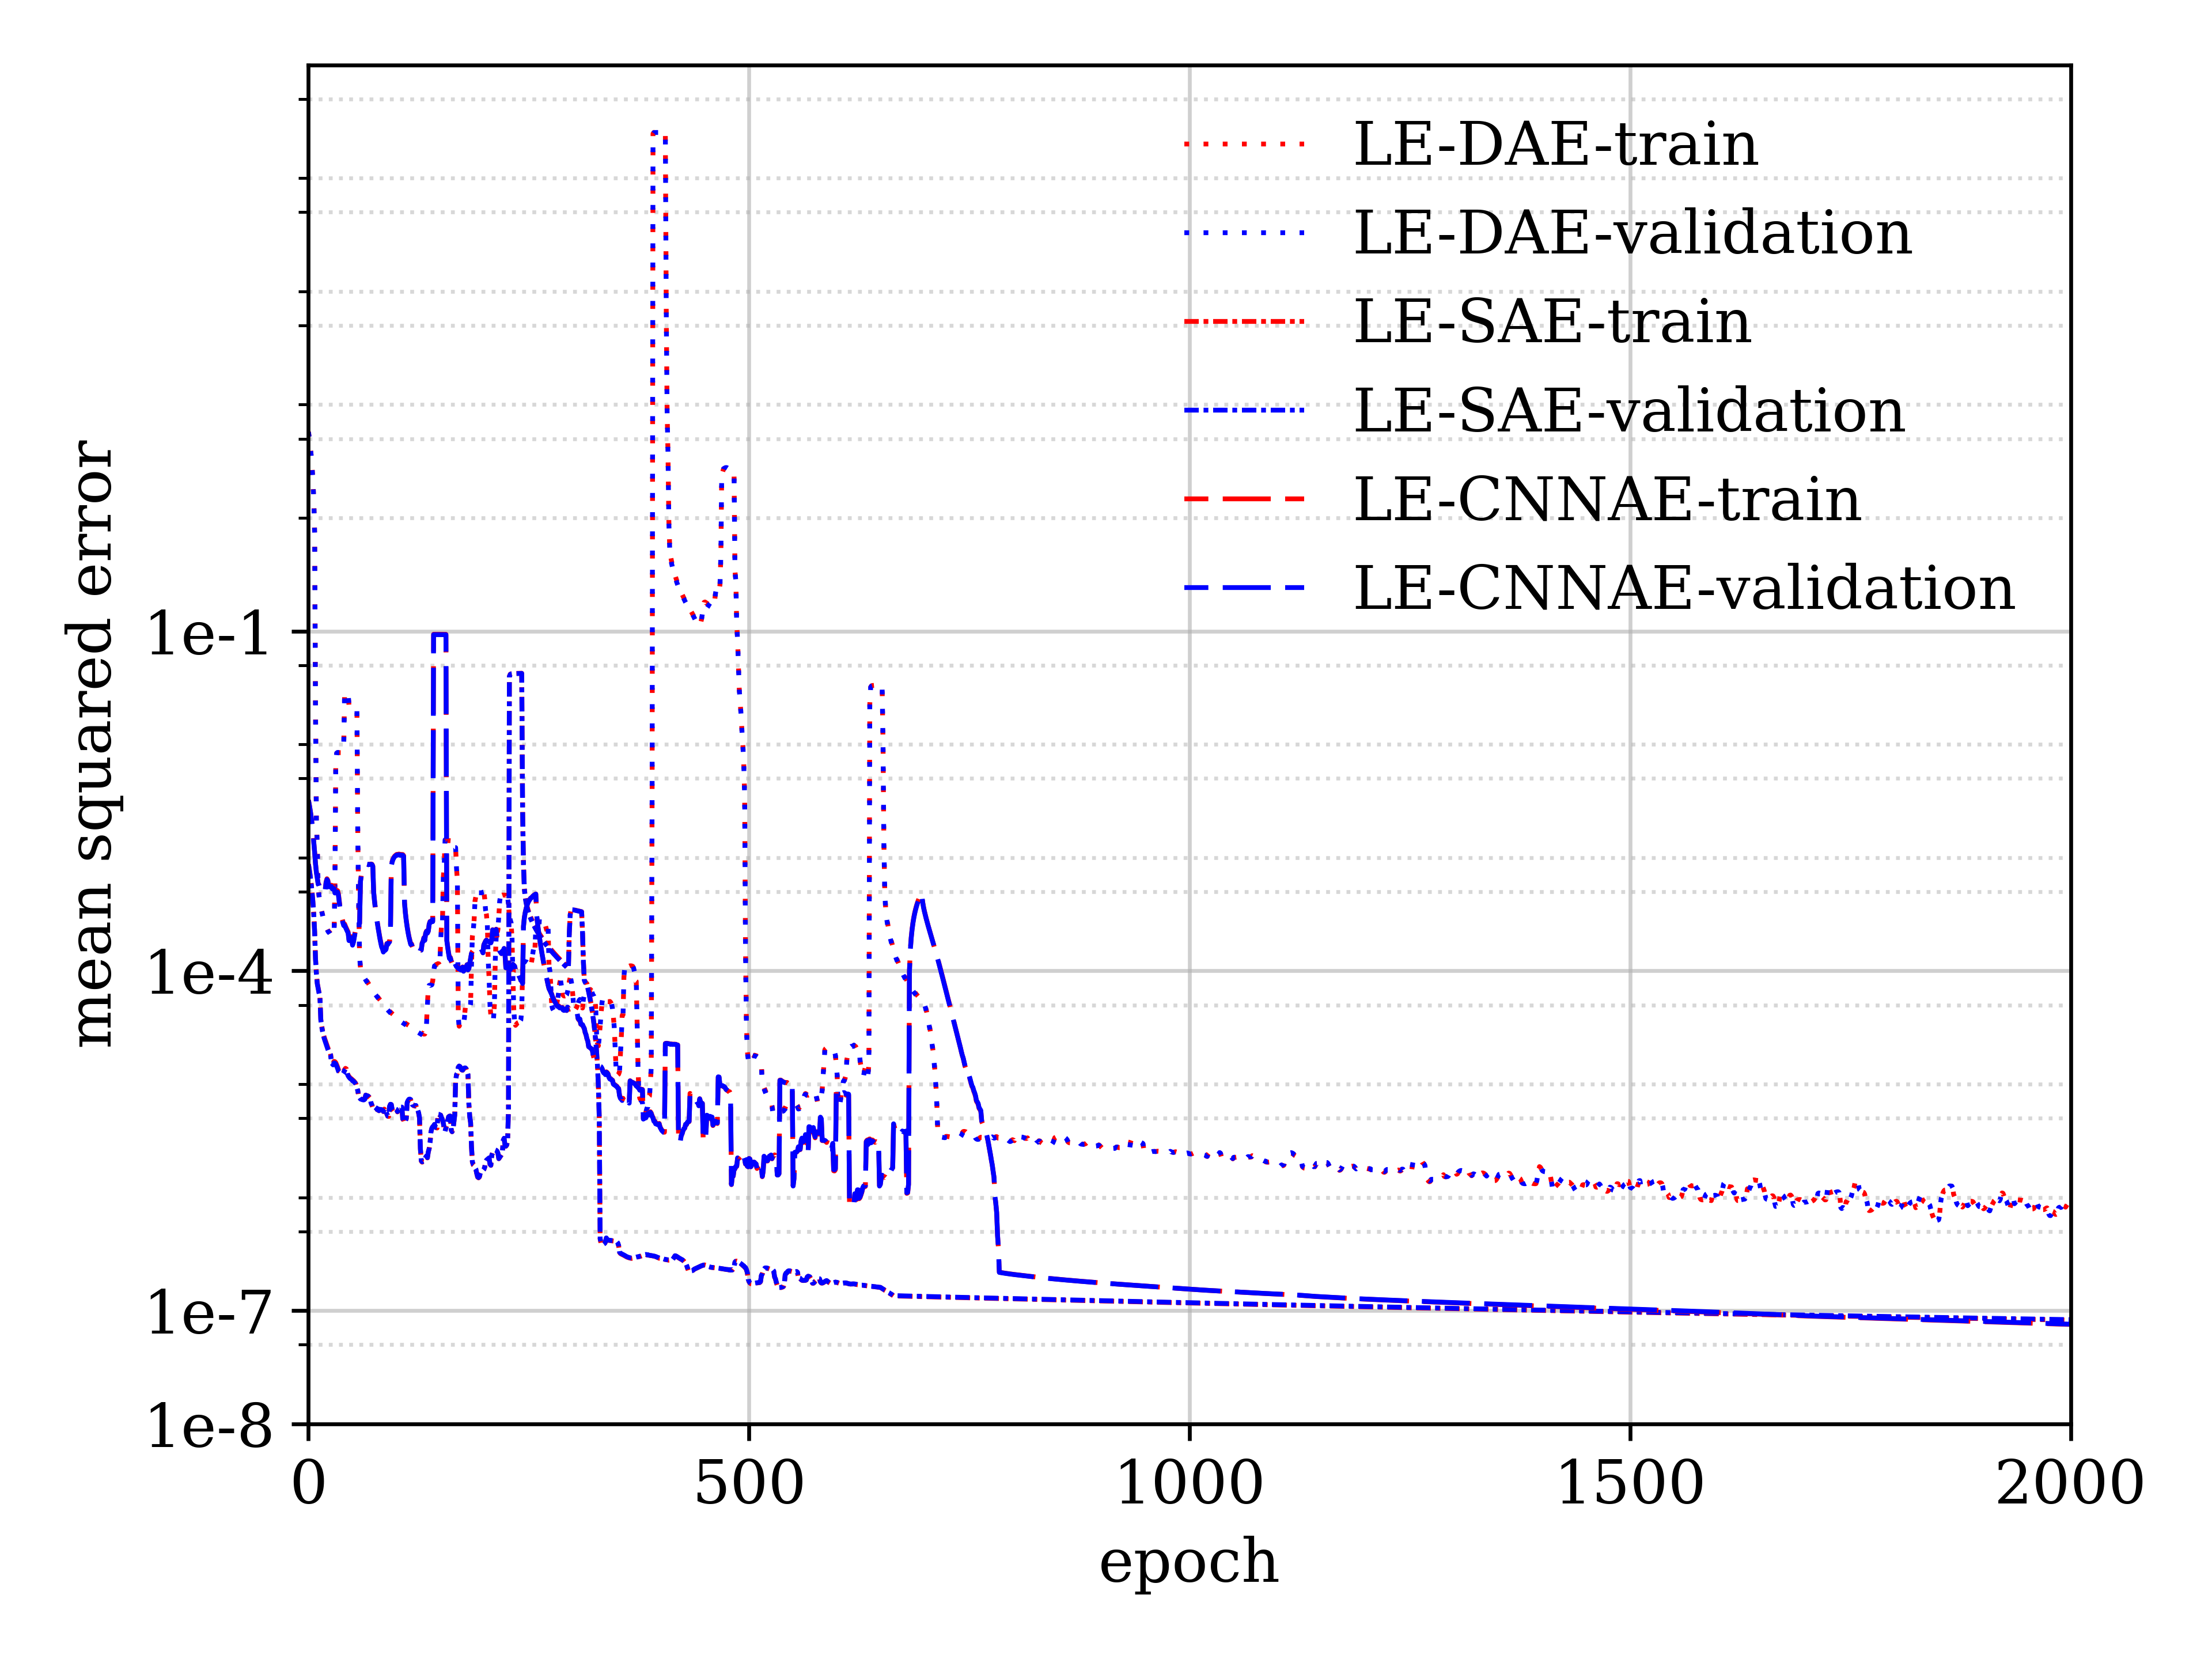
\includegraphics[width=\textwidth]{LE_train_test_history_autoencoder.png}
            \end{center}
            \caption{}
        \end{subfigure}
        \begin{subfigure}[b]{0.49\textwidth}
           \begin{center}
            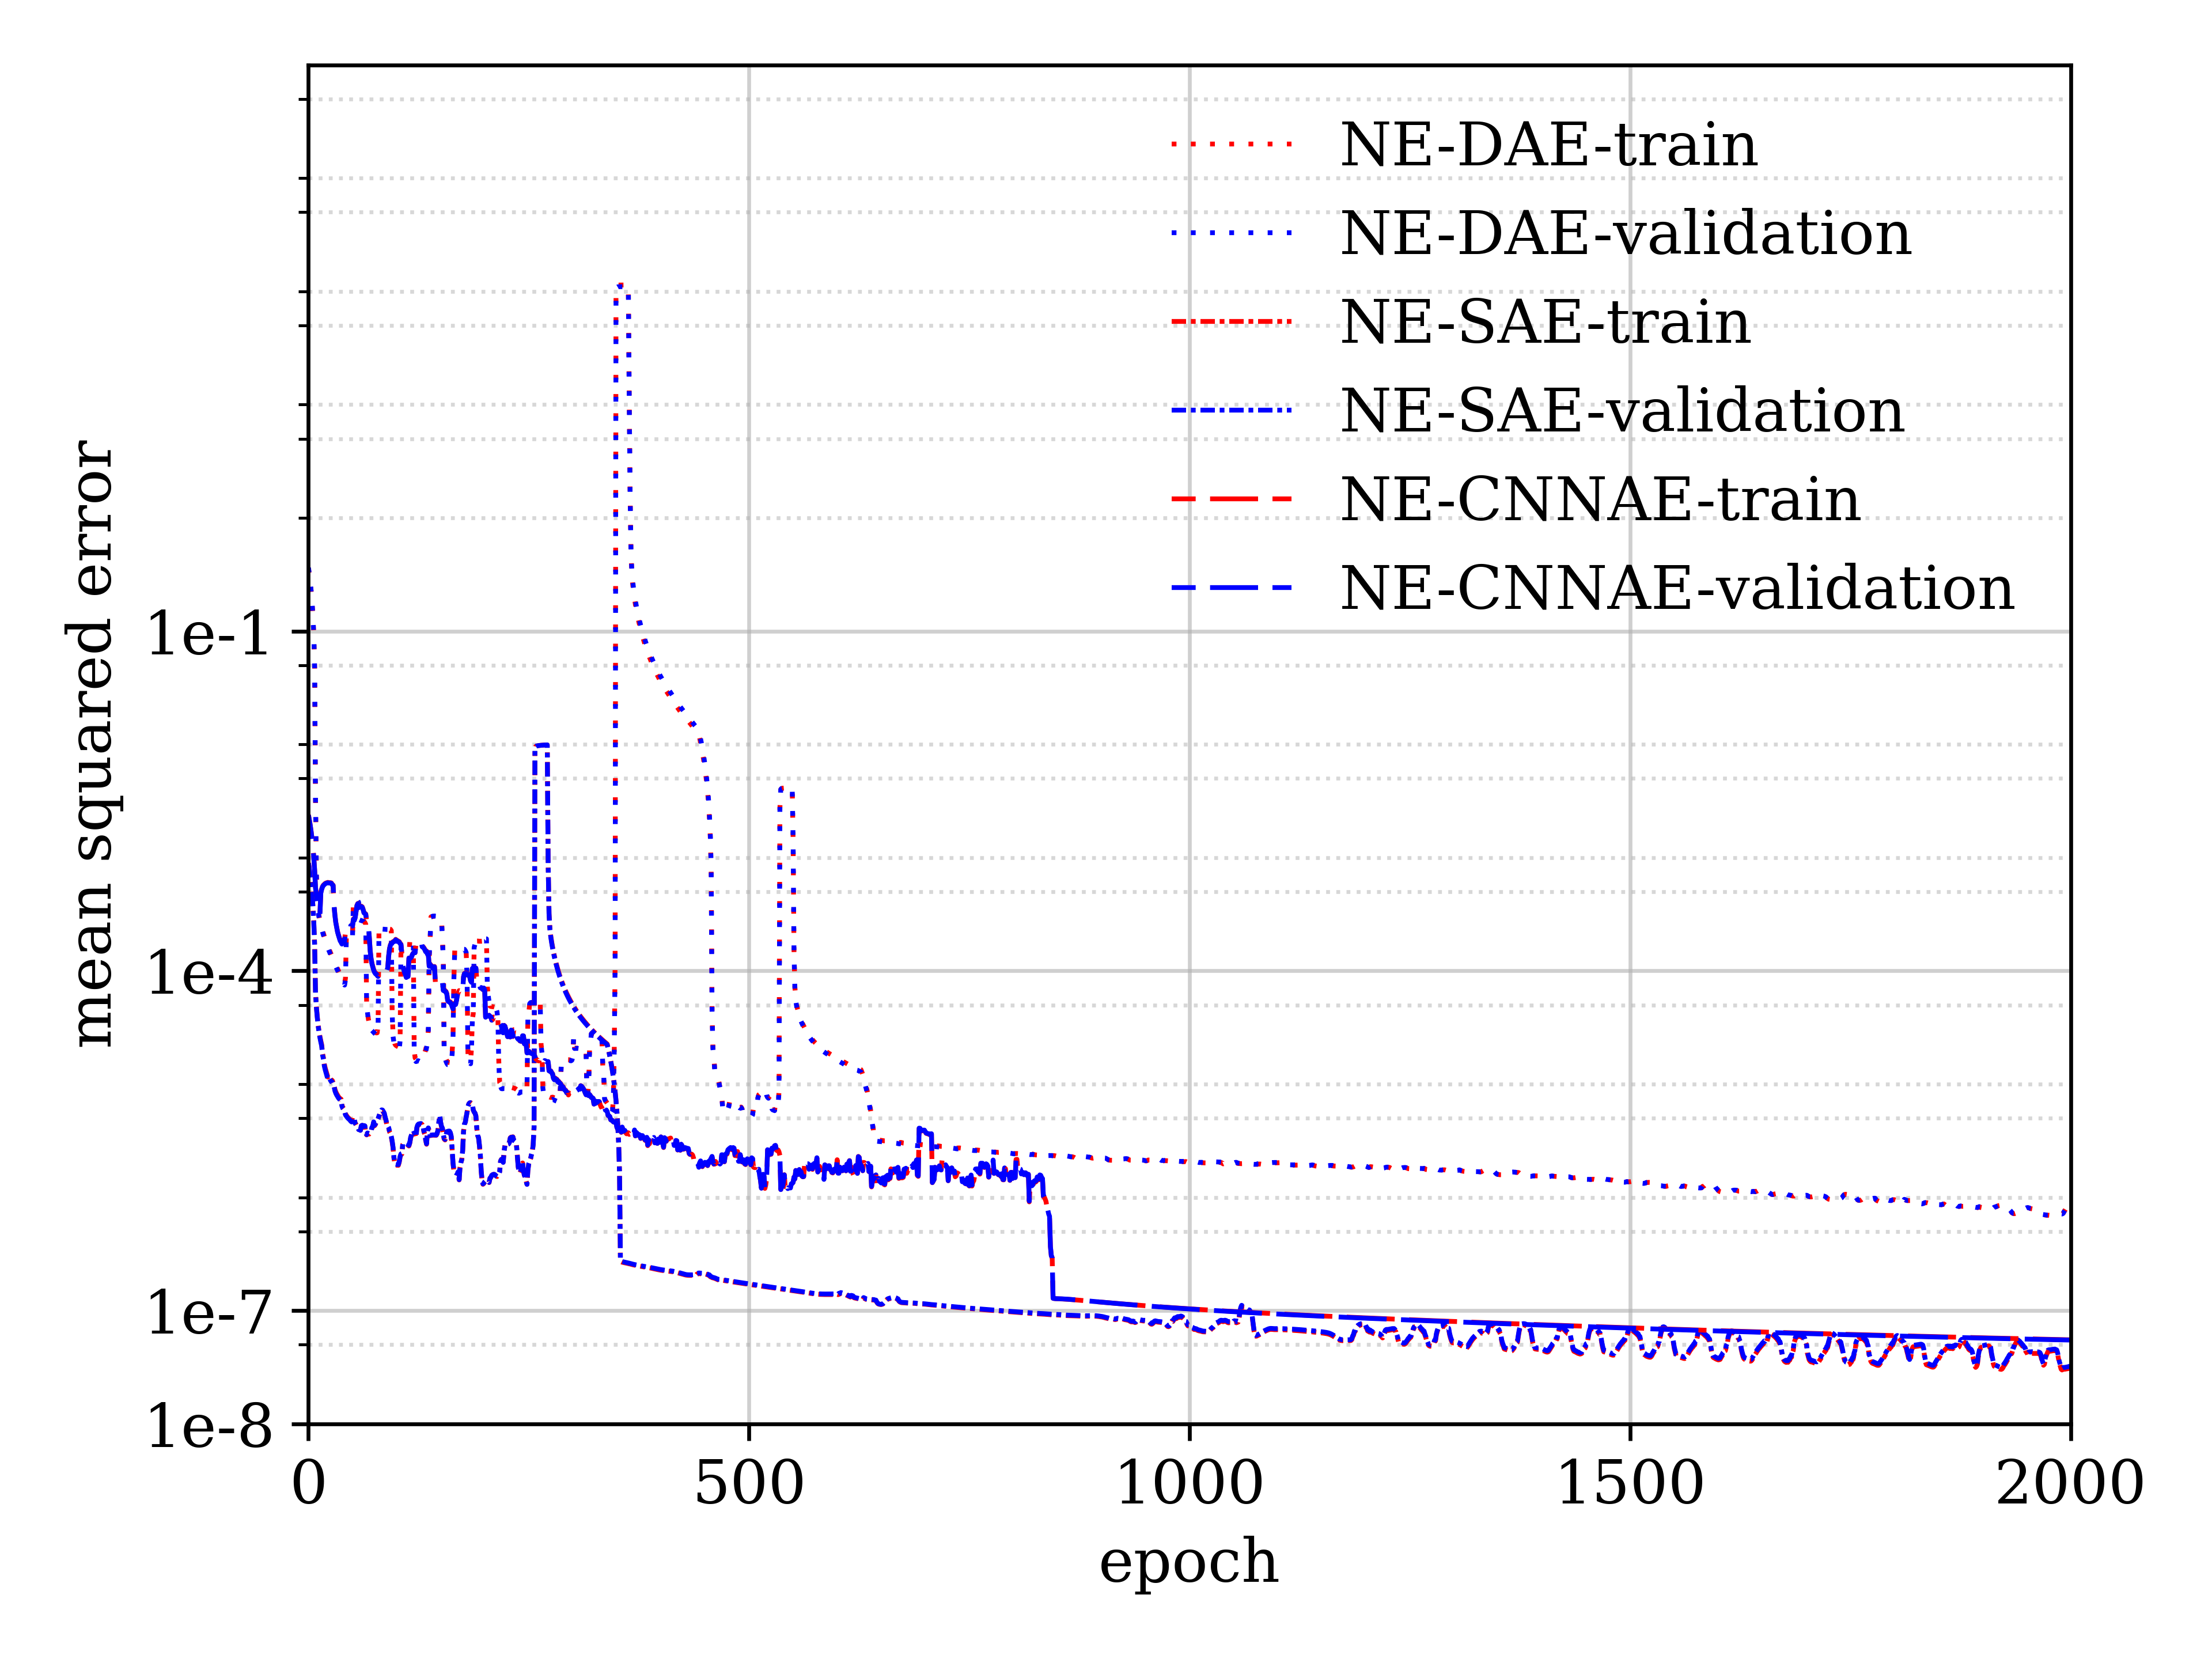
\includegraphics[width=\textwidth]{NE_train_test_history_autoencoder.png}
           \end{center}
            \caption{}
        \end{subfigure}
     \end{center}
        \caption[Loss history ($r = 20$) for the autoencoders.]{Loss (training and validation) history ($r = 20$) for the deep autoencoder (DAE), the sparse autoencoder (SAE), and the proposed convolutional autoencoder (CNNAE) with linear (a) and nonlinear encoder (b). Savitzky-Golay filter is applied to the loss history for better visualization, with filter window length equals to 15, the order of the polynomial used to fit the loss is 1, and the extension contains the nearest input value.}
        \label{fig: train test history}
\end{figure}

We consider the \textit{projection errors} of the autoencoders defined as 
\begin{align}
    l^{\text{proj}}_{\text{LAE}}(\btU; \btPhi) = \frac{\sqrt{\sum_{l=1}^{N_{ic}}\sum_{m=0}^{N_t}\norm{\btu^{\left<m\right>}(u_0^{(\ell)}) - \bar{\btu} - \sum_{i=1}^{r} \inner{\mathbb{R}^N}{\btu^{\left<m\right>}(u_0^{(\ell)}) - \bar{\btu}}{\btphi_i}\btphi_i}^2}}{\sqrt{\sum_{l=1}^{N_{ic}}\sum_{m=0}^{N_t}\norm{\btu^{\left<m\right>}(u_0^{(\ell)})}^2}}
\end{align}
and
\begin{align}
    l^{\text{proj}}_{\text{NAE}}(\btU; \boldsymbol{\Theta}_e, \boldsymbol{\Theta}_d) = \frac{\sqrt{\sum_{l=1}^{N_{ic}}\sum_{m=0}^{N_t}\norm{\btu^{\left<m\right>}(u_0^{(\ell)}) - \bar{\btu} - D(E(\btu^{\left<m\right>}(u_0^{(\ell)}) - \bar{\btu}; \boldsymbol{\Theta}_e); \boldsymbol{\Theta}_d)}^2}}{\sqrt{\sum_{l=1}^{N_{ic}}\sum_{m=0}^{N_t}\norm{\btu^{\left<m\right>}(u_0^{(\ell)})}^2}}\,,
\end{align}
for the linear and nonlinear autoencoders, respectively. The projection error for all autoencoders on the test dataset ($\mu = 1.0$) over different latent space dimensions $r \in \{5, 10, 15, 20\}$ is summarized in Fig.~\ref{fig: proj err burger}.
\begin{figure}[!htb]
    \begin{center}
        \begin{subfigure}[b]{0.49\textwidth}
           \begin{center}
            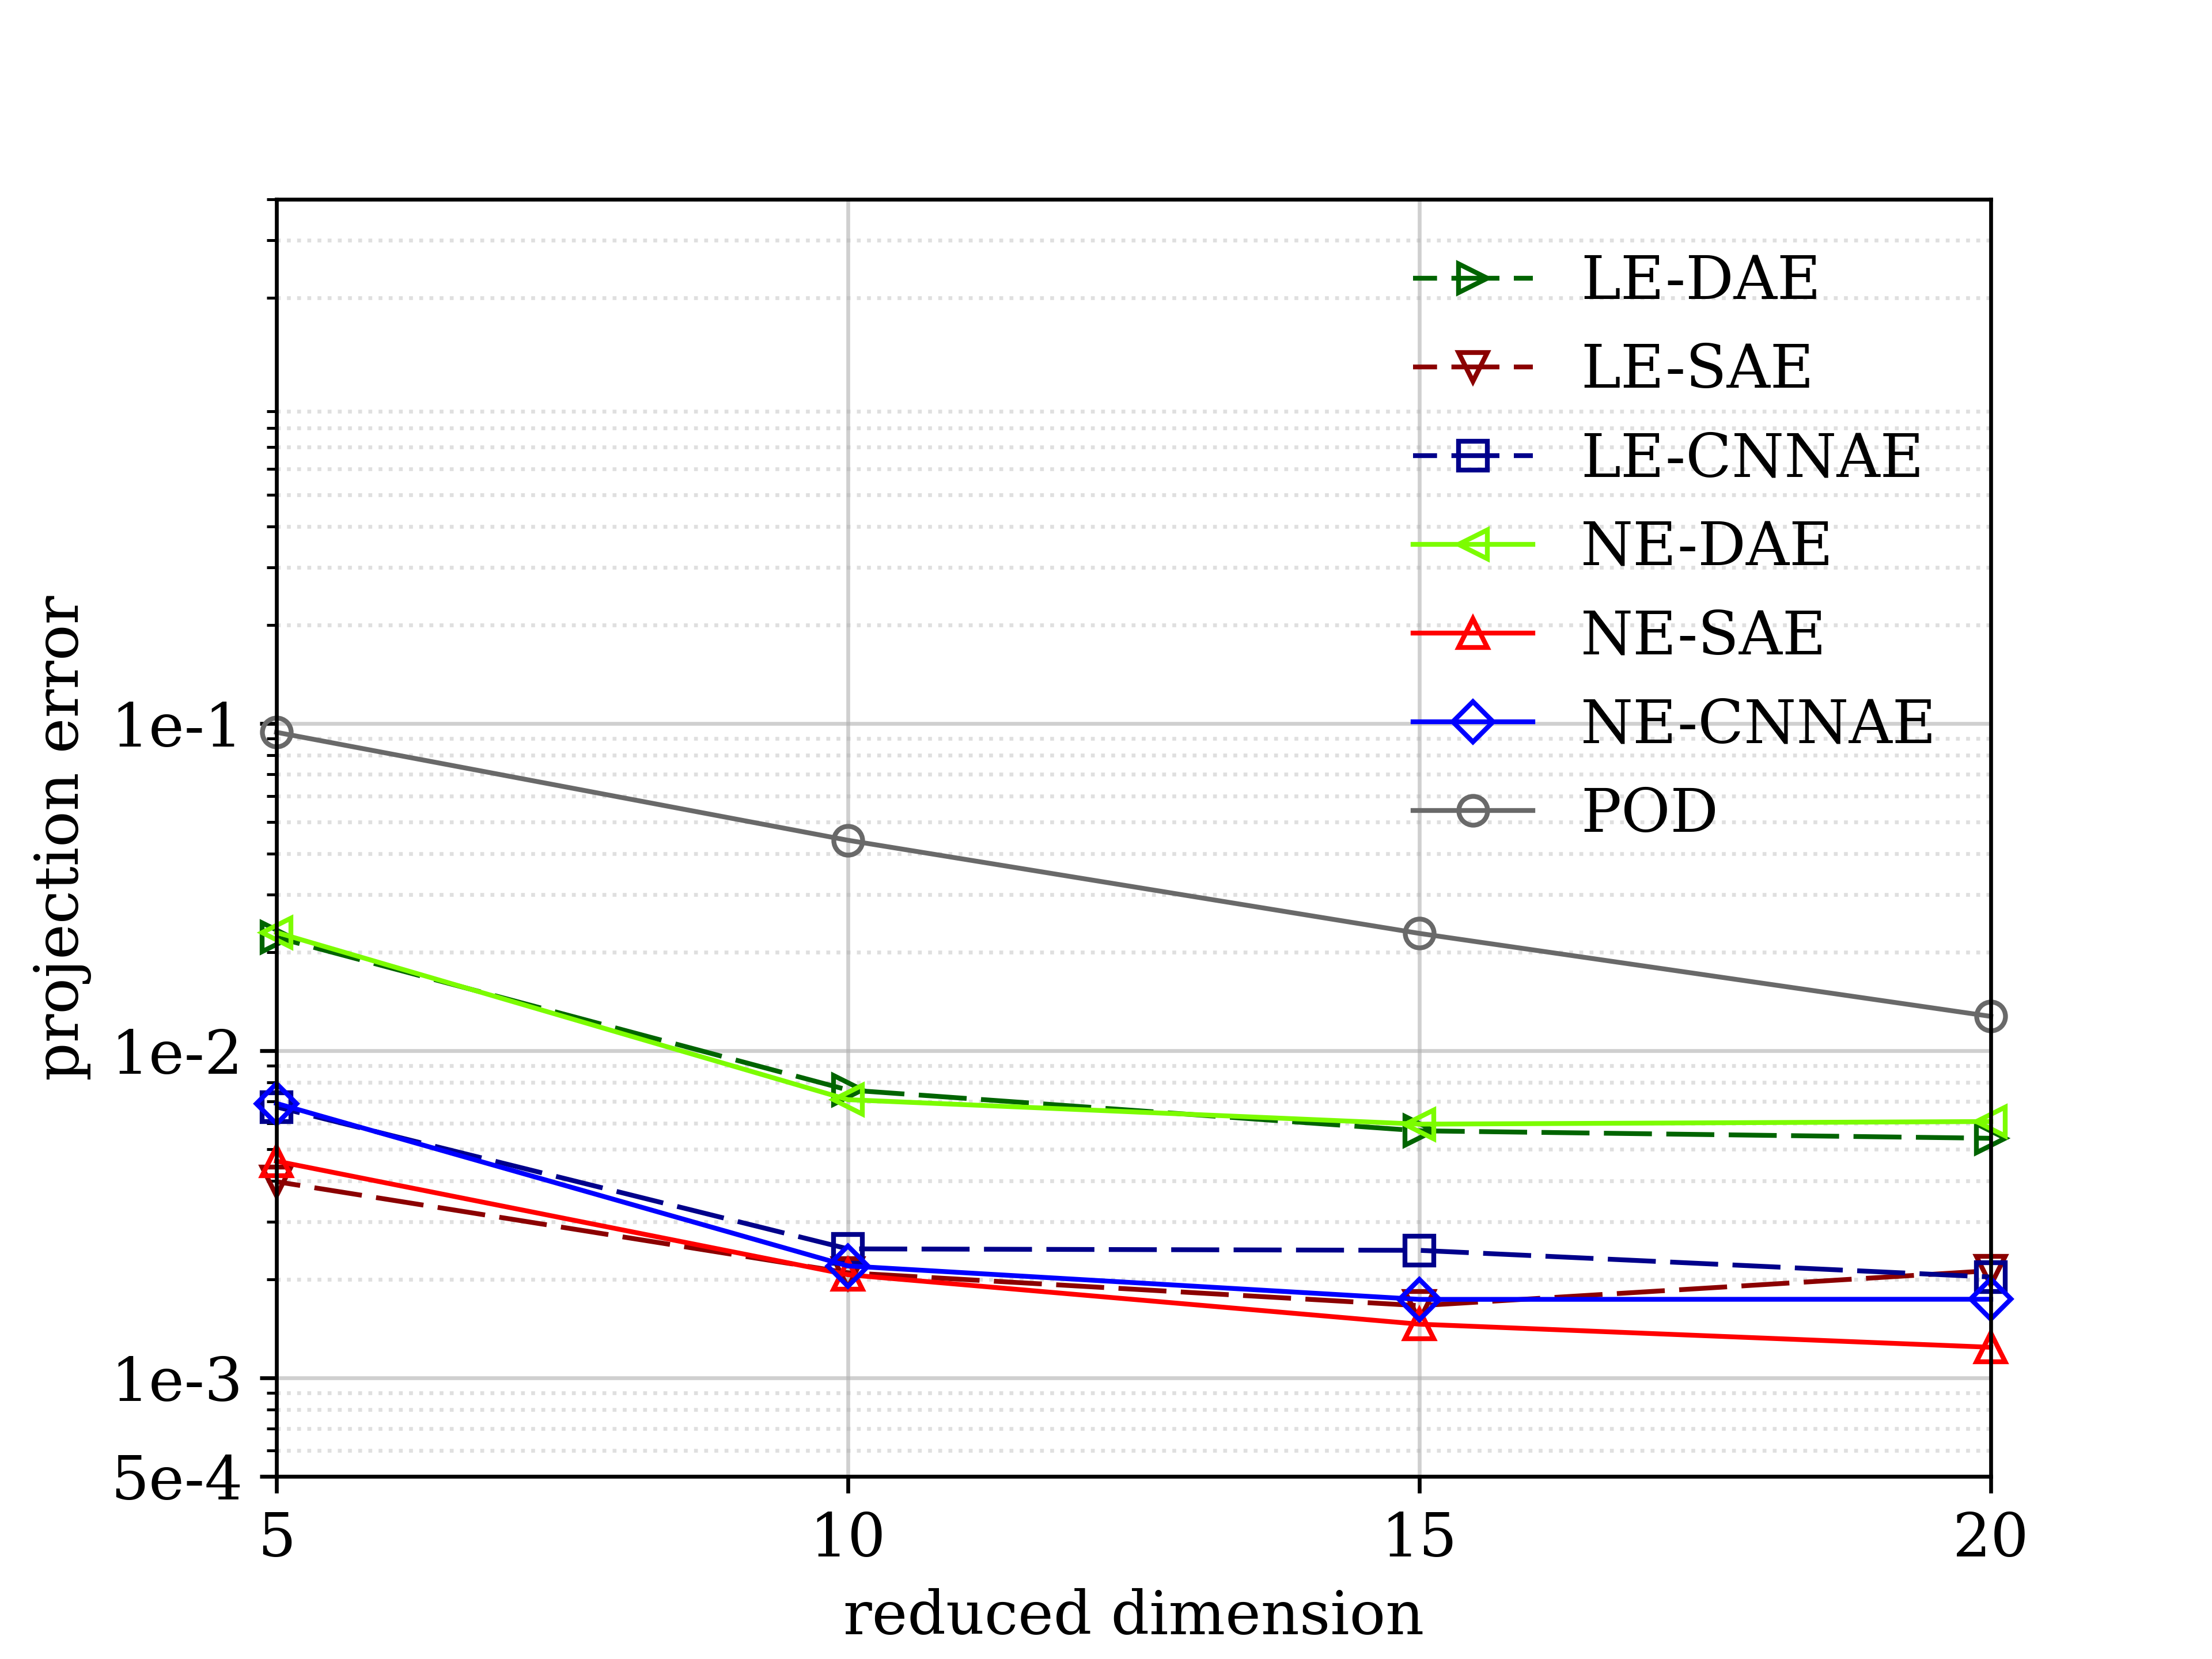
\includegraphics[width=\textwidth]{proj_err_autoencoder_train.png}
           \end{center}
            \caption{}
            \label{fig: proj err burger train}
        \end{subfigure}
        \begin{subfigure}[b]{0.49\textwidth}
            \begin{center}
           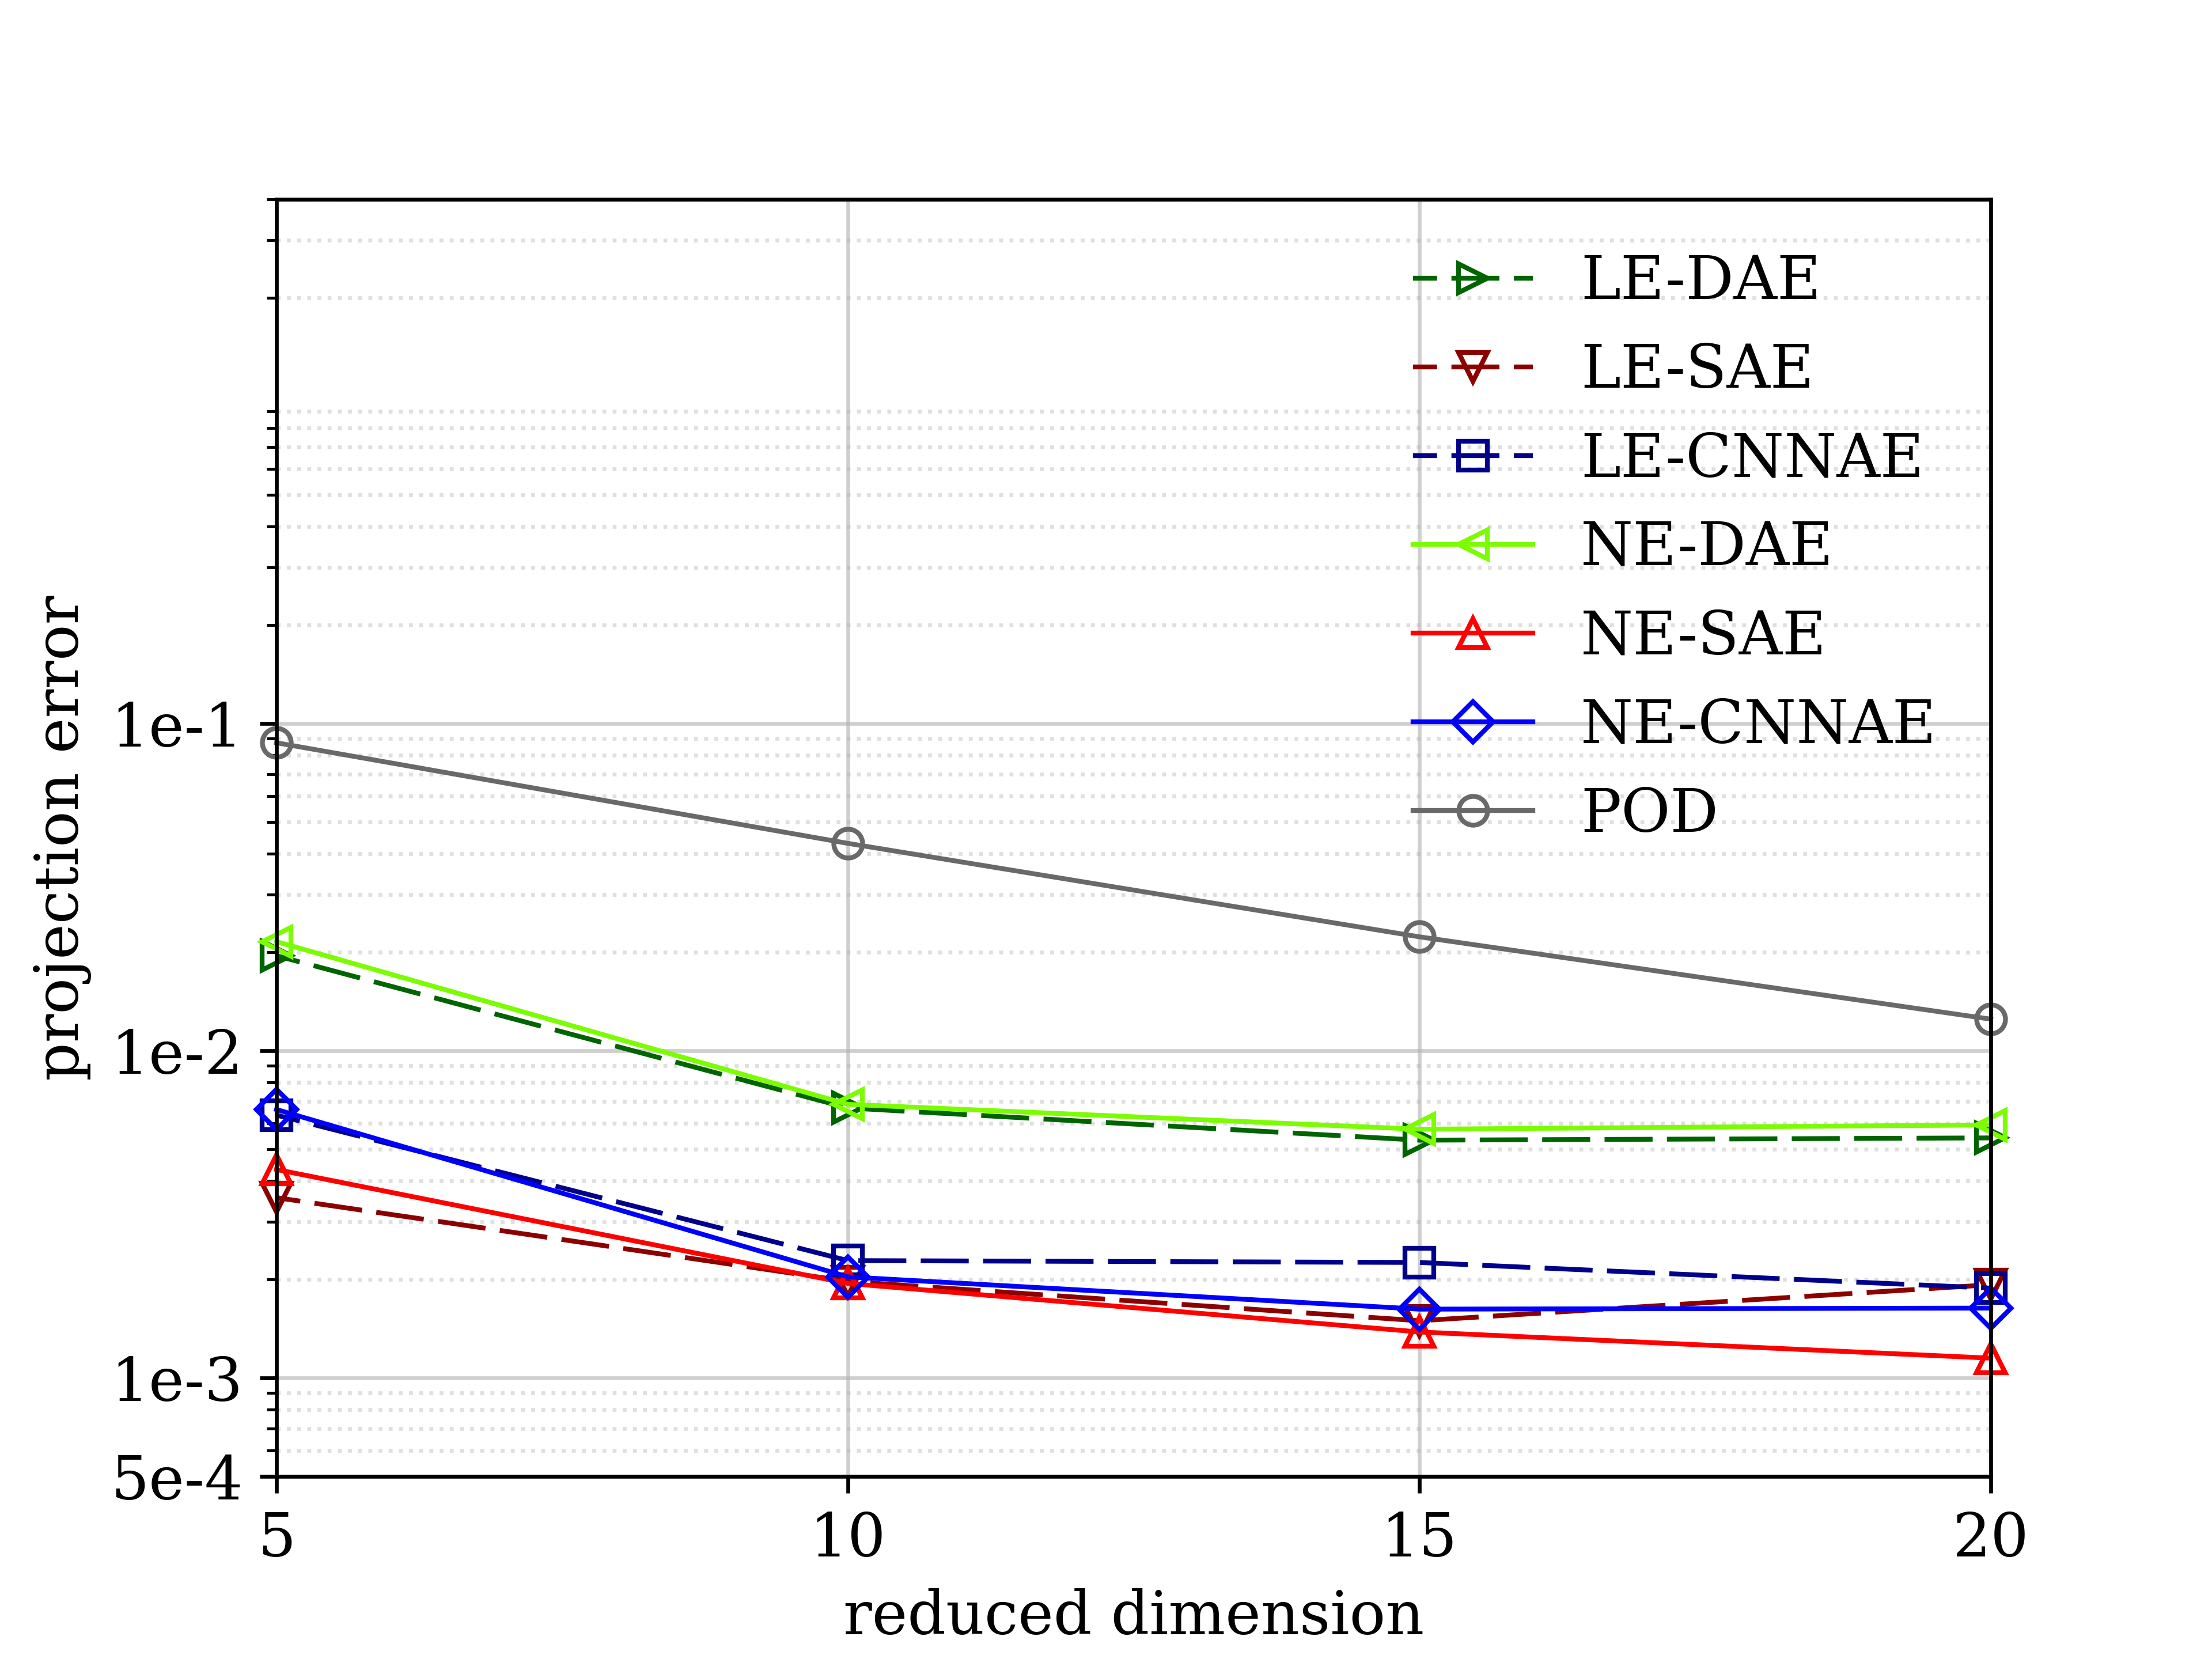
\includegraphics[width=\textwidth]{proj_err_autoencoder.png}
            \end{center}
            \caption{}
            \label{fig: proj err burger}
        \end{subfigure}
    \end{center}
        \caption[Projection error and training and test data.]{(a) Projection error over different latent space dimensions on training data with $\mu = \{0.9, 0.95, 1.05, 1.1\}$; (b) Projection error over different latent space dimensions on test data with $\mu = 1.0$.}
\end{figure}

\subsection{Training of Reduced Operators}
We consider two strategies for operator learning between latent spaces. For OPInf, we solve Eq.~\eqref{eq:opinf} for the linear and quadratic reduced operators. For DNNOp, we use 5 hidden layers with sizes of $M_o = 50$, and the swish function as the activation function. The model is trained for 2000 epochs, using the Adam optimizer and an initial learning rate set to $0.01$. We split the training dataset into $n_{\text{batch}} = 100$ batches, and use maximum patience of 100 epochs such that the learning rate will decrease by a factor of 10 when the maximum patience is reached. The reduced operators are trained and paired with the autoencoders given different latent space dimensions, and the training and validation loss (projection error on the rate between latent spaces) histories with r = 20 for all autoencoders paired with the reduced operator are shown in Fig.~\ref{fig: ML op train test history}. Again, it is seen that the training and validation losses exhibit very similar trends and magnitudes, with a good balance between accuracy and overfitting. In Fig.~\ref{fig: operator projection error}, we summarize the projection error of the trained reduced operator given different latent space dimensions. The projection error between latent spaces of the reduced operator is defined as
\begin{align}
    l^{\text{proj}}_{\text{LQ}}(\hat{\btU}; \btA, \btH) = \frac{\sqrt{\sum_{l=1}^{N_{ic}}\sum_{m=0}^{N_t}\norm{\dot{\hat{\btu}}^{\left<m\right>}(u_0^{(\ell)}) - \btA\hat{\btu}^{\left<m\right>} + \btH \left(\hat{\btu}^{\left<m\right>} \otimes \hat{\btu}^{\left<m\right>}\right); \boldsymbol{\Theta}_o)}^2}}{\sqrt{\sum_{l=1}^{N_{ic}}\sum_{m=0}^{N_t}\norm{\dot{\hat{\btu}}^{\left<m\right>}(u_0^{(\ell)})}^2}}\,,
\end{align}
and
\begin{align}
    l^{\text{proj}}_{\text{DNNOp}}(\hat{\btU}; \boldsymbol{\Theta}_o) = \frac{\sqrt{\sum_{l=1}^{N_{ic}}\sum_{m=0}^{N_t}\norm{\dot{\hat{\btu}}^{\left<m\right>}(u_0^{(\ell)}) - \rtO(\hat{\btu}^{\left<m\right>}(u_0^{(\ell)}); \boldsymbol{\Theta}_o)}^2}}{\sqrt{\sum_{l=1}^{N_{ic}}\sum_{m=0}^{N_t}\norm{\dot{\hat{\btu}}^{\left<m\right>}(u_0^{(\ell)})}^2}}\,,
\end{align}
for the quadratic operator inference and DNN-based operator, respectively.

\begin{figure}[!htb]
     \begin{center}
        \begin{subfigure}[b]{0.49\textwidth}
            \begin{center}
            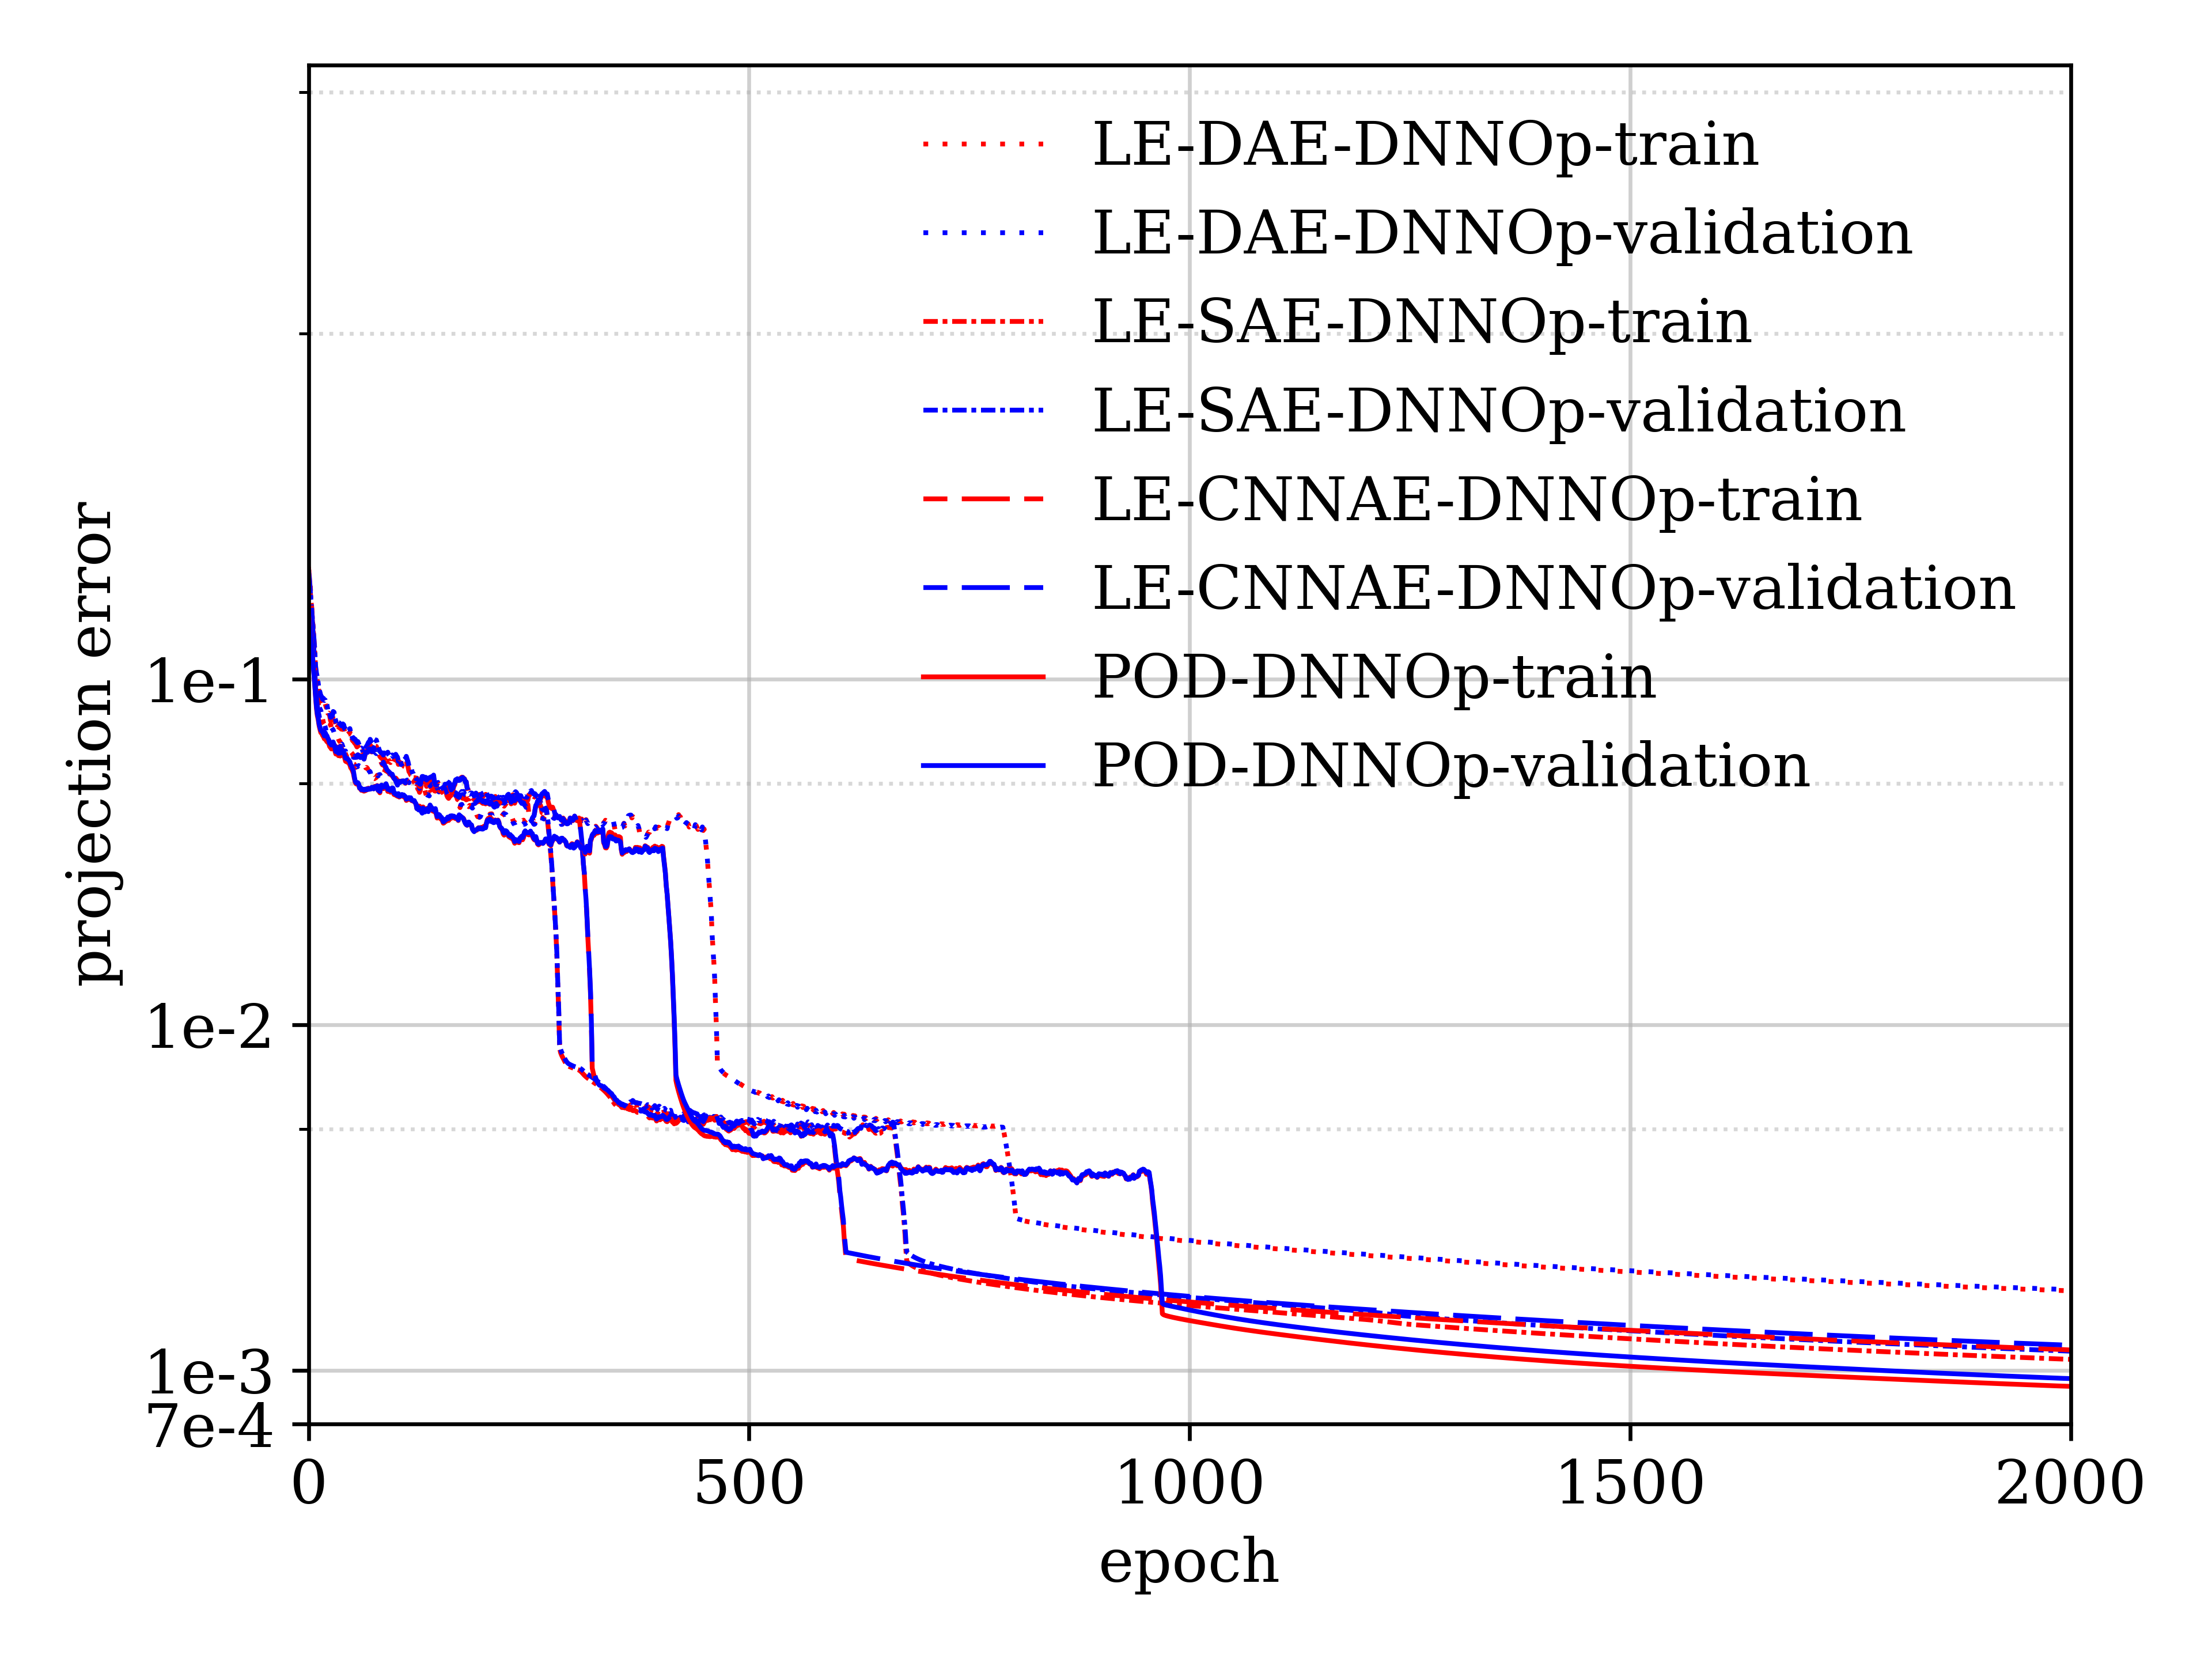
\includegraphics[width=\textwidth]{LE_train_test_history_op.png}
            \end{center}
            \caption{}
        \end{subfigure}
        \begin{subfigure}[b]{0.49\textwidth}
           \begin{center}
            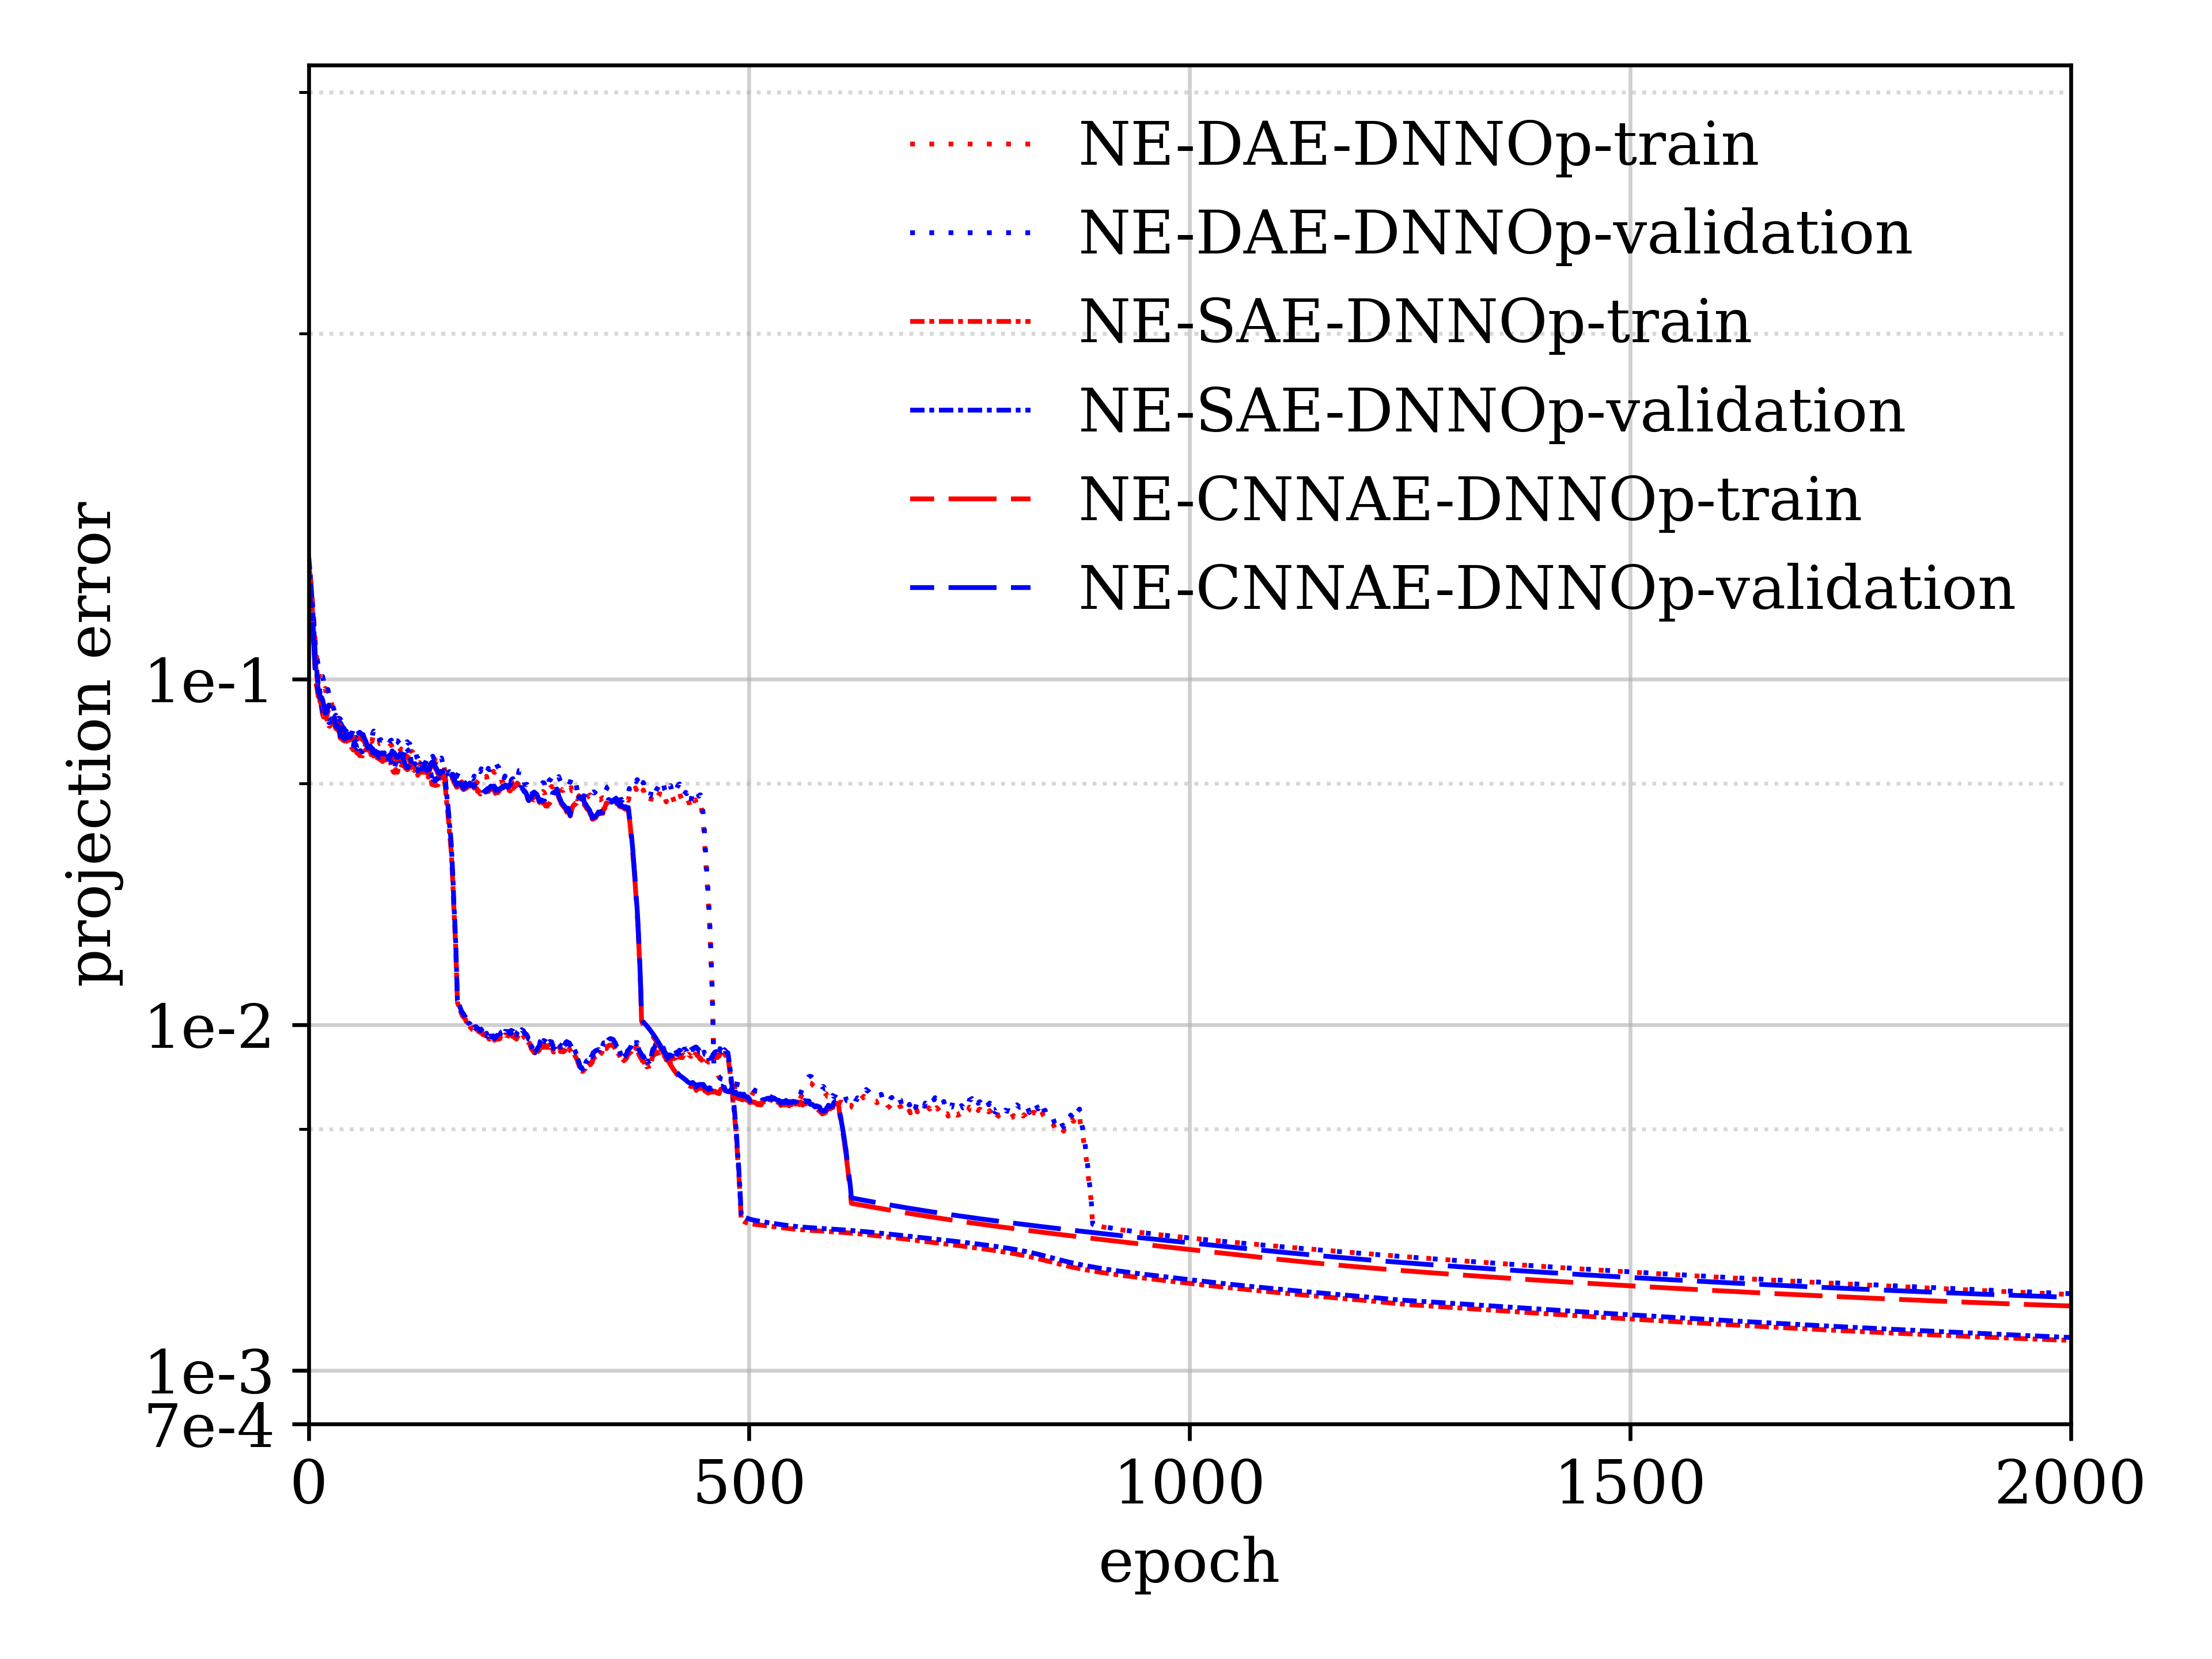
\includegraphics[width=\textwidth]{NE_train_test_history_op.png}
           \end{center}
            \caption{}
        \end{subfigure}
     \end{center}
        \caption[Loss history ($r = 20$) of DNNOp paired with autoencoders.]{Loss (training and validation) history ($r = 20$) of DNNOp paired with linear (a) and nonlinear encoders (b) as well as POD (a). Savitzky-Golay filter is applied to the loss history for better visualization, with filter window length equals to 15, the order of the polynomial used to fit the loss is 1, and the extension contains the nearest input value.}
        \label{fig: ML op train test history}
\end{figure}

\begin{figure}[!htb]
     \begin{center}
        \begin{subfigure}[b]{0.49\textwidth}
            \begin{center}
            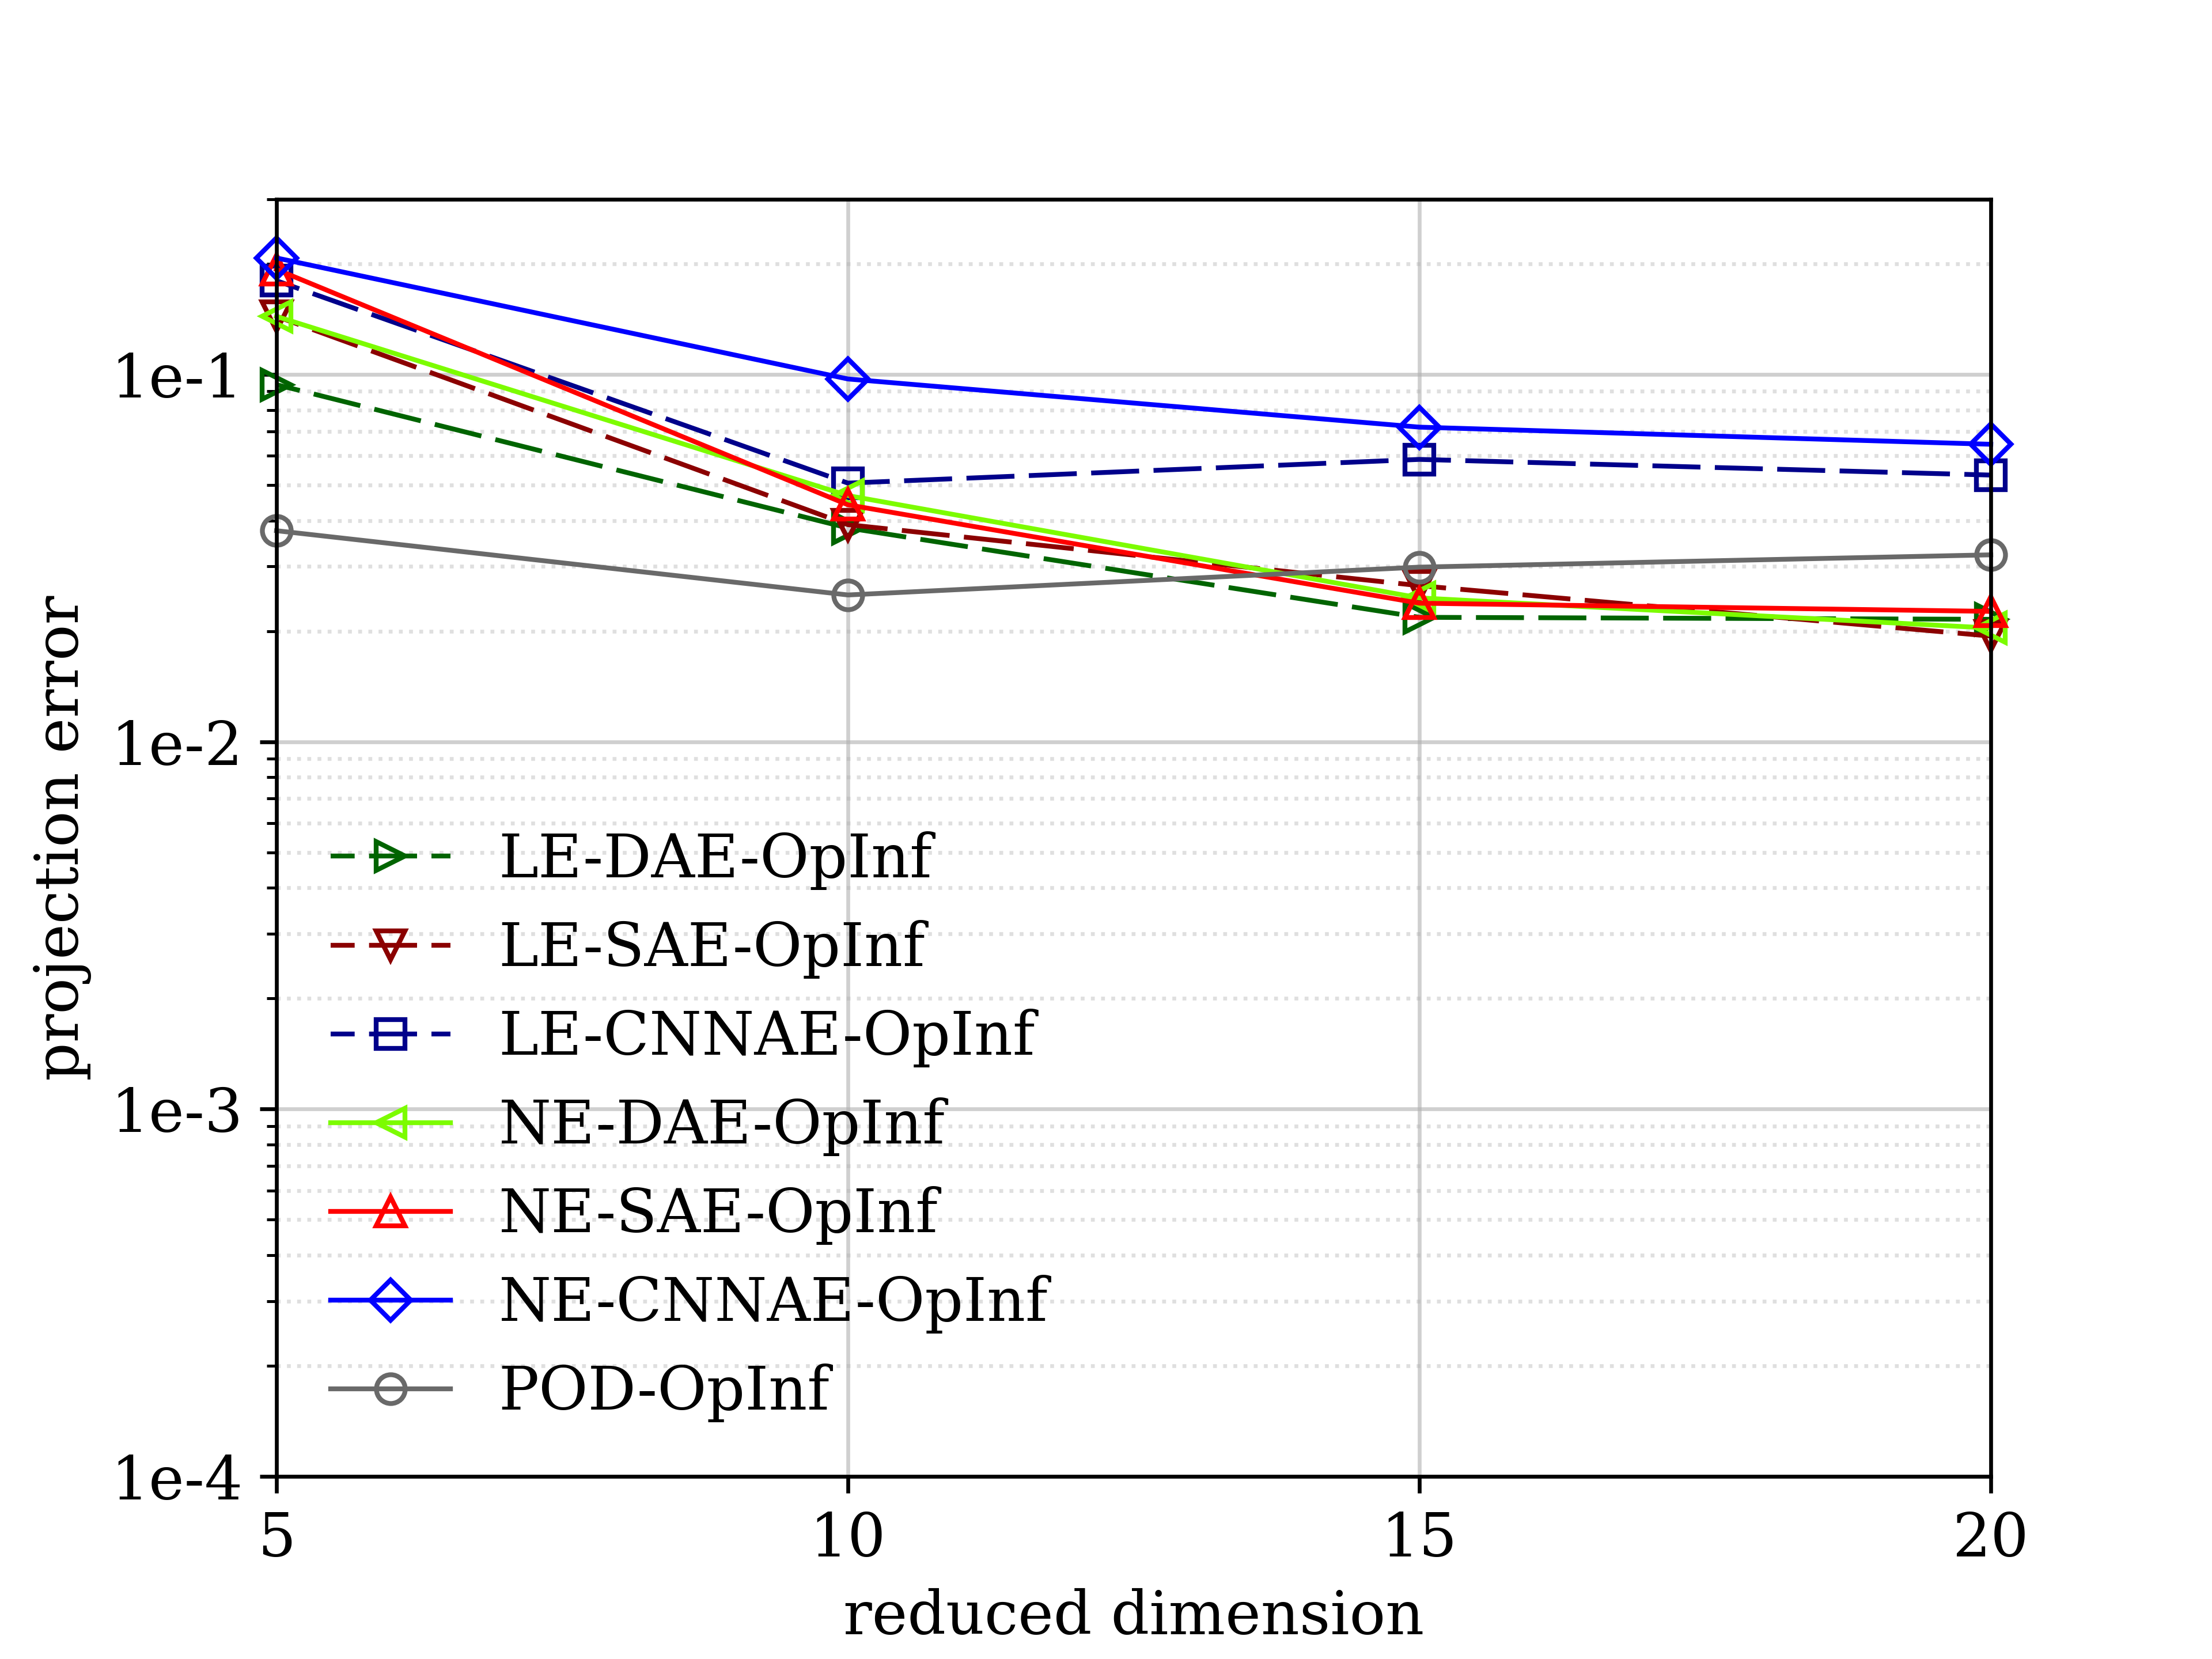
\includegraphics[width=\textwidth]{proj_err_operator_train_opinf.png}
            \end{center}
            \caption{}
        \end{subfigure}
        \begin{subfigure}[b]{0.49\textwidth}
            \begin{center}
           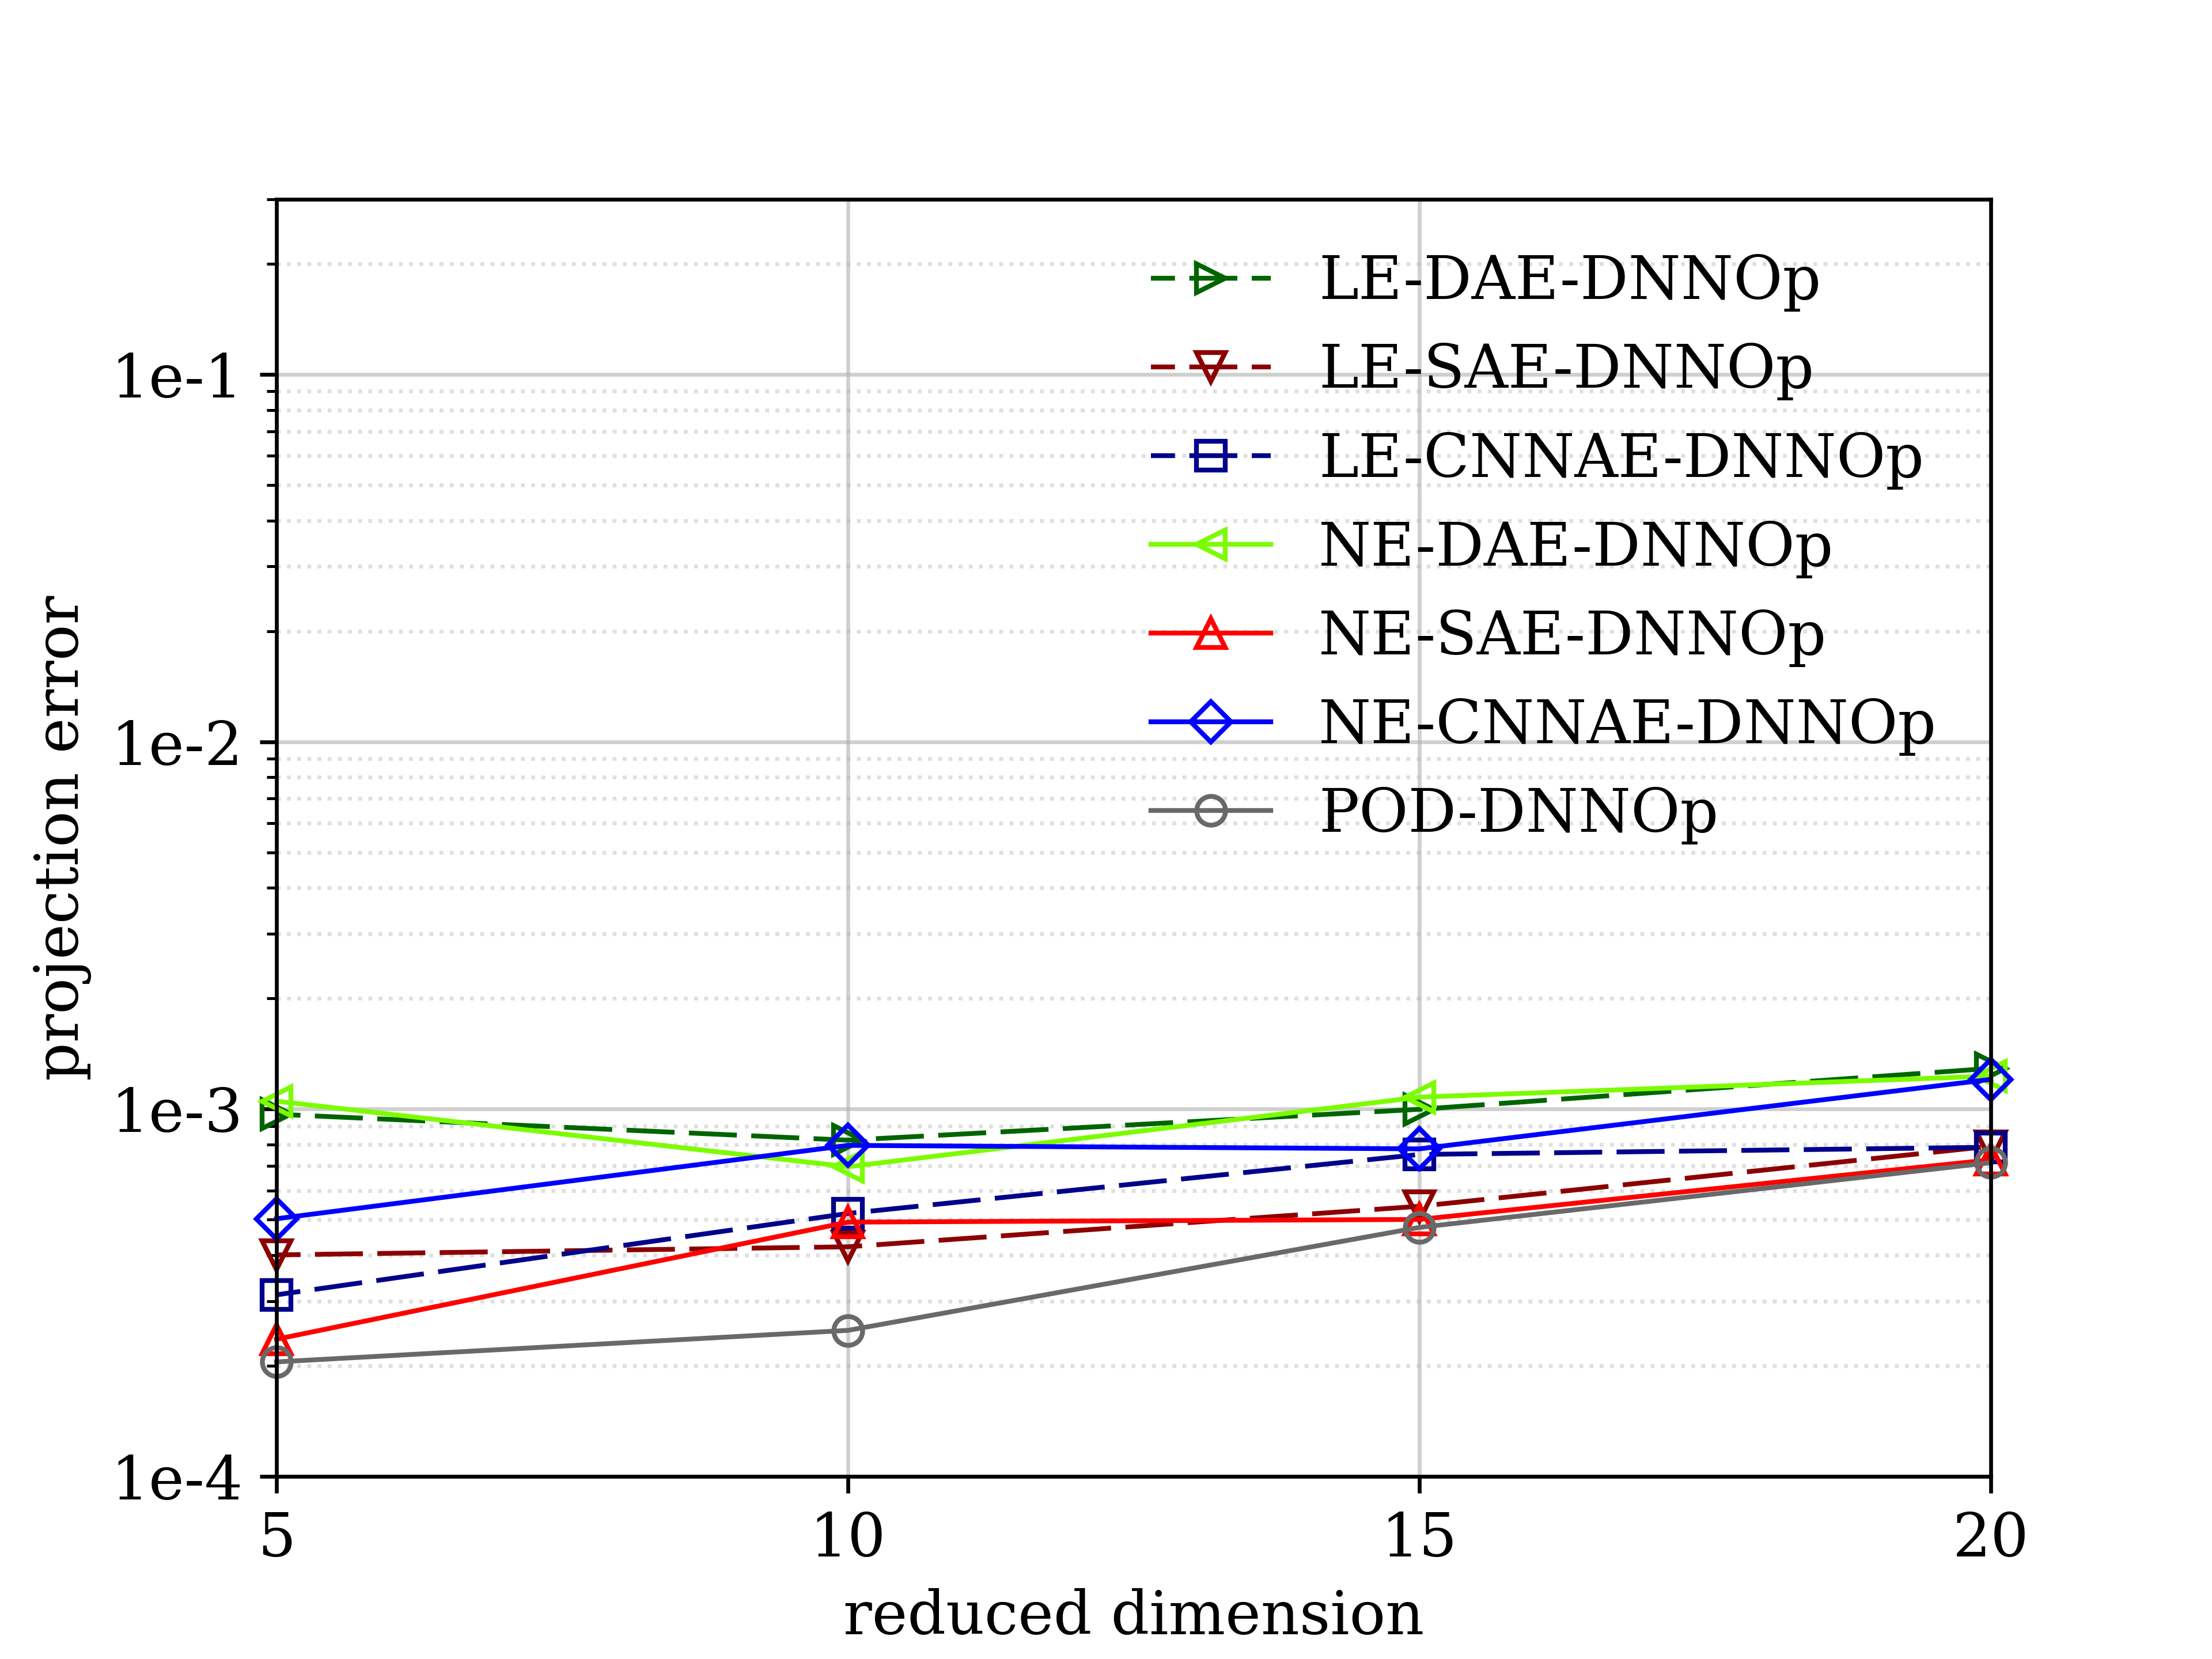
\includegraphics[width=\textwidth]{proj_err_operator_train_dnnop.png}
            \end{center}
            \caption{}
        \end{subfigure}
     \end{center}
        \caption[Projection error of the trained reduced operators.]{Projection error of the trained reduced operator $F$ in the latent spaces for (a) quadratic operator inference; and (b) DNN-based operator on the training dataset with $\mu = \{0.9, 0.95, 1.01, 1.1\}$.}
        \label{fig: operator projection error}
\end{figure}

We evaluate the reduced operators' performances between the latent spaces (i.e., the flow map $u_0 \mapsto u(\cdot, t)$, $t > 0$) on the test dataset using the errors given by
\begin{align}
    l^{\text{proj}}_{rom}(\hat{\btU}; \hat{\btu}_0, \boldsymbol{\Theta}_o) = \frac{\sqrt{\sum_{l=1}^{N_{ic}}\sum_{m=0}^{N_t}\norm{\hat{\btu}^{\left<m\right>}(u_0^{(\ell)}) - \hat{\btu}^{\left<m\right>}_{rom}(u_0^{(\ell)})}^2}}{\sqrt{\sum_{l=1}^{N_{ic}}\sum_{m=0}^{N_t}\norm{\hat{\btu}^{\left<m\right>}(u_0^{(\ell)})}^2}}\,,
\end{align}
where $\hat{\btu}^{\left<m\right>}_{rom}(u_0^{(\ell)}) = \mathcal{H}(\hat{\btu}_0(u_0^{(\ell)}); \boldsymbol{\Theta}_o, t_m)$ is the approximated latent solution at a given time step $m$. We solve the reduced order model using the Newton-Raphson method. We evaluate the reduced-order model solution obtained by combining the surrogate operator $\mathcal{H}$ with any of the autoencoders with a projection error in the original high dimensional space, using the error defined as
\begin{align}
    l^{\text{proj}}_{\text{sol}}(\btU; \btPhi, \mathcal{H}(\boldsymbol{\Theta}_o)) = \frac{\sqrt{\sum_{l=1}^{N_{ic}}\sum_{m=0}^{N_t}\norm{\btu^{\left<m\right>}(u_0^{(\ell)}) - \bar{\btu} - \sum_{i=1}^{r} \mathcal{H}(\hat{\btu}_0(u_0^{(\ell)}); \boldsymbol{\Theta}_o, t^m)\btphi_i}^2}}{\sqrt{\sum_{l=1}^{N_{ic}}\sum_{m=0}^{N_t}\norm{\btu^{\left<m\right>}(u_0^{(\ell)})}^2}}
\end{align}
and
\begin{align}
    l^{\text{proj}}_{\text{sol}}(\btU; \boldsymbol{\Theta}_e, \boldsymbol{\Theta}_d, \mathcal{H}(\boldsymbol{\Theta}_o)) = \frac{\sqrt{\sum_{l=1}^{N_{ic}}\sum_{m=0}^{N_t}\norm{\btu^{\left<m\right>}(u_0^{(\ell)}) - \bar{\btu} - D(\mathcal{H}(\hat{\btu}_0(u_0^{(\ell)}); \boldsymbol{\Theta}_o, t^m); \boldsymbol{\Theta}_d)}^2}}{\sqrt{\sum_{l=1}^{N_{ic}}\sum_{m=0}^{N_t}\norm{\btu^{\left<m\right>}(u_0^{(\ell)})}^2}}\,,
\end{align}
for the linear and nonlinear autoencoders, respectively, with $\hat{\btu}_0(u_0^{(\ell)}) = E(\btu_0(u_0^{(\ell)}); \boldsymbol{\Theta}_e)$.

In Fig.~\ref{fig: proj err rom solution}, we show the projection error for the reduced-order model solution over all latent dimensions with different pairs of autoencoders and operators. Note that quadratic operator inference fails to solve this 2D Burger's problem with an error blowing up for $m > 200$ approximately.
\begin{figure}[!htb]
     \begin{center}
        \begin{subfigure}[b]{0.49\textwidth}
            \begin{center}
            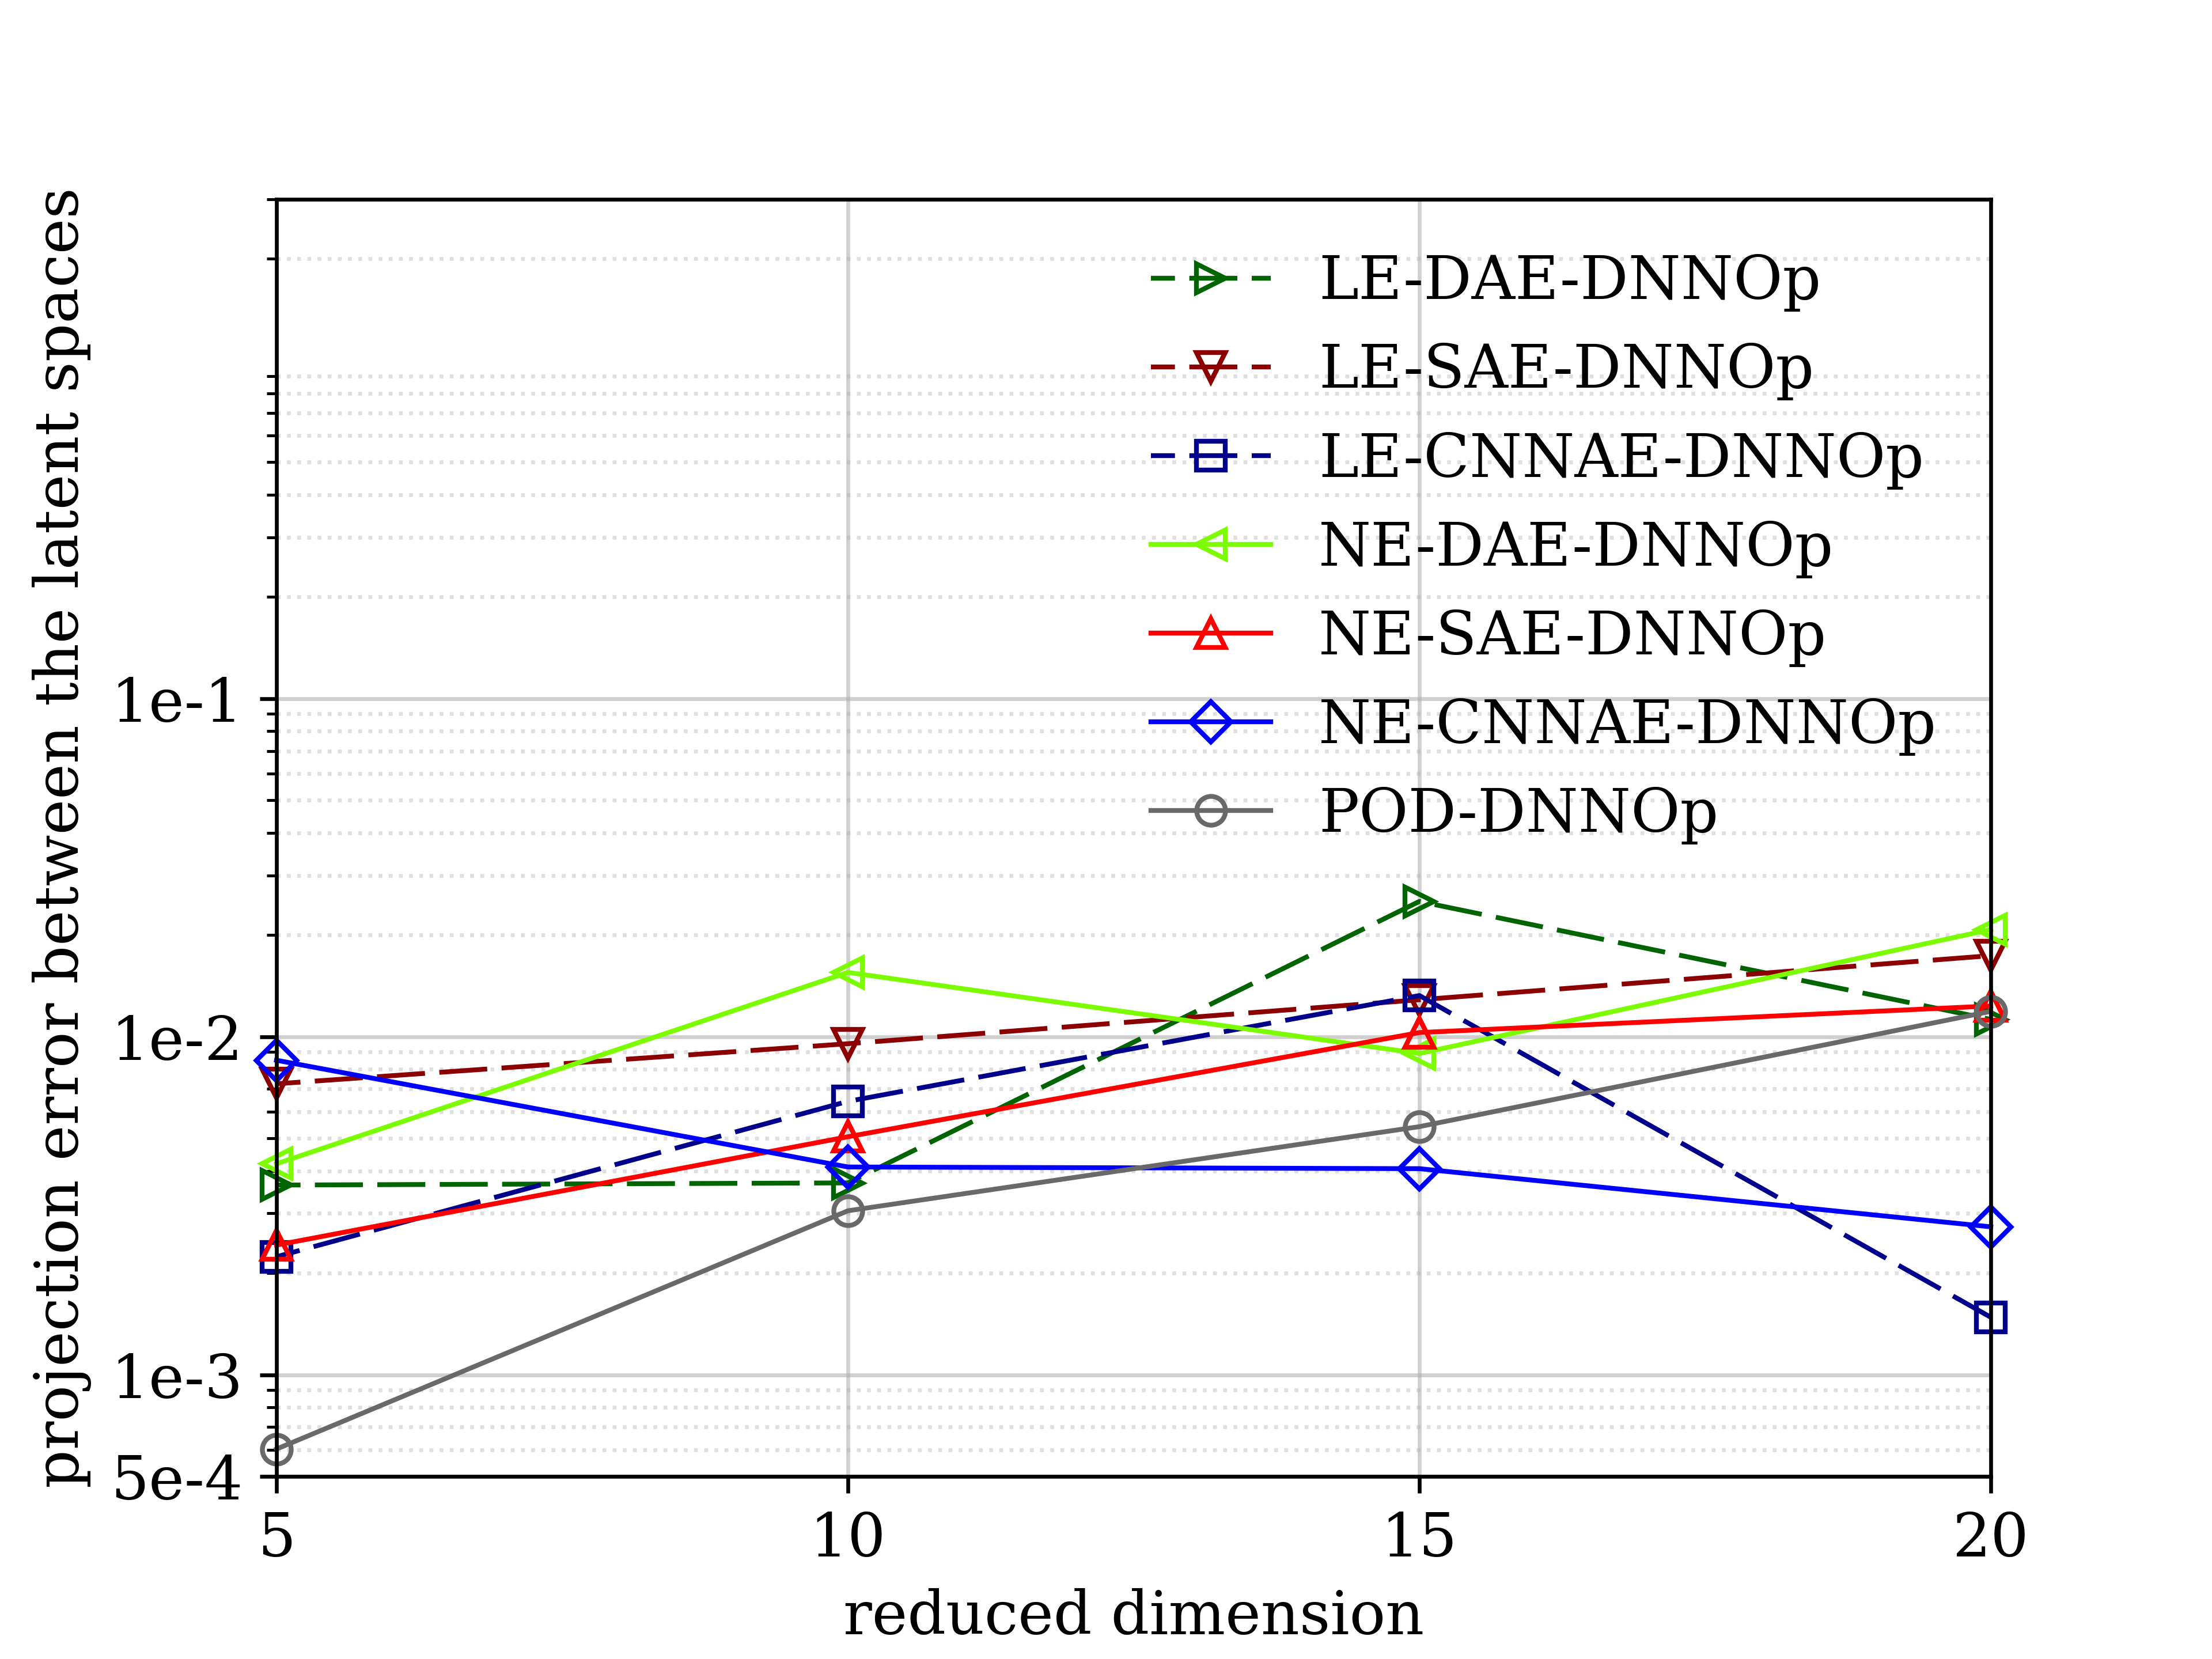
\includegraphics[width=\textwidth]{proj_err_xhat_validation.png}
            \end{center}
            \caption{}
        \end{subfigure}
        \begin{subfigure}[b]{0.49\textwidth}
            \begin{center}
           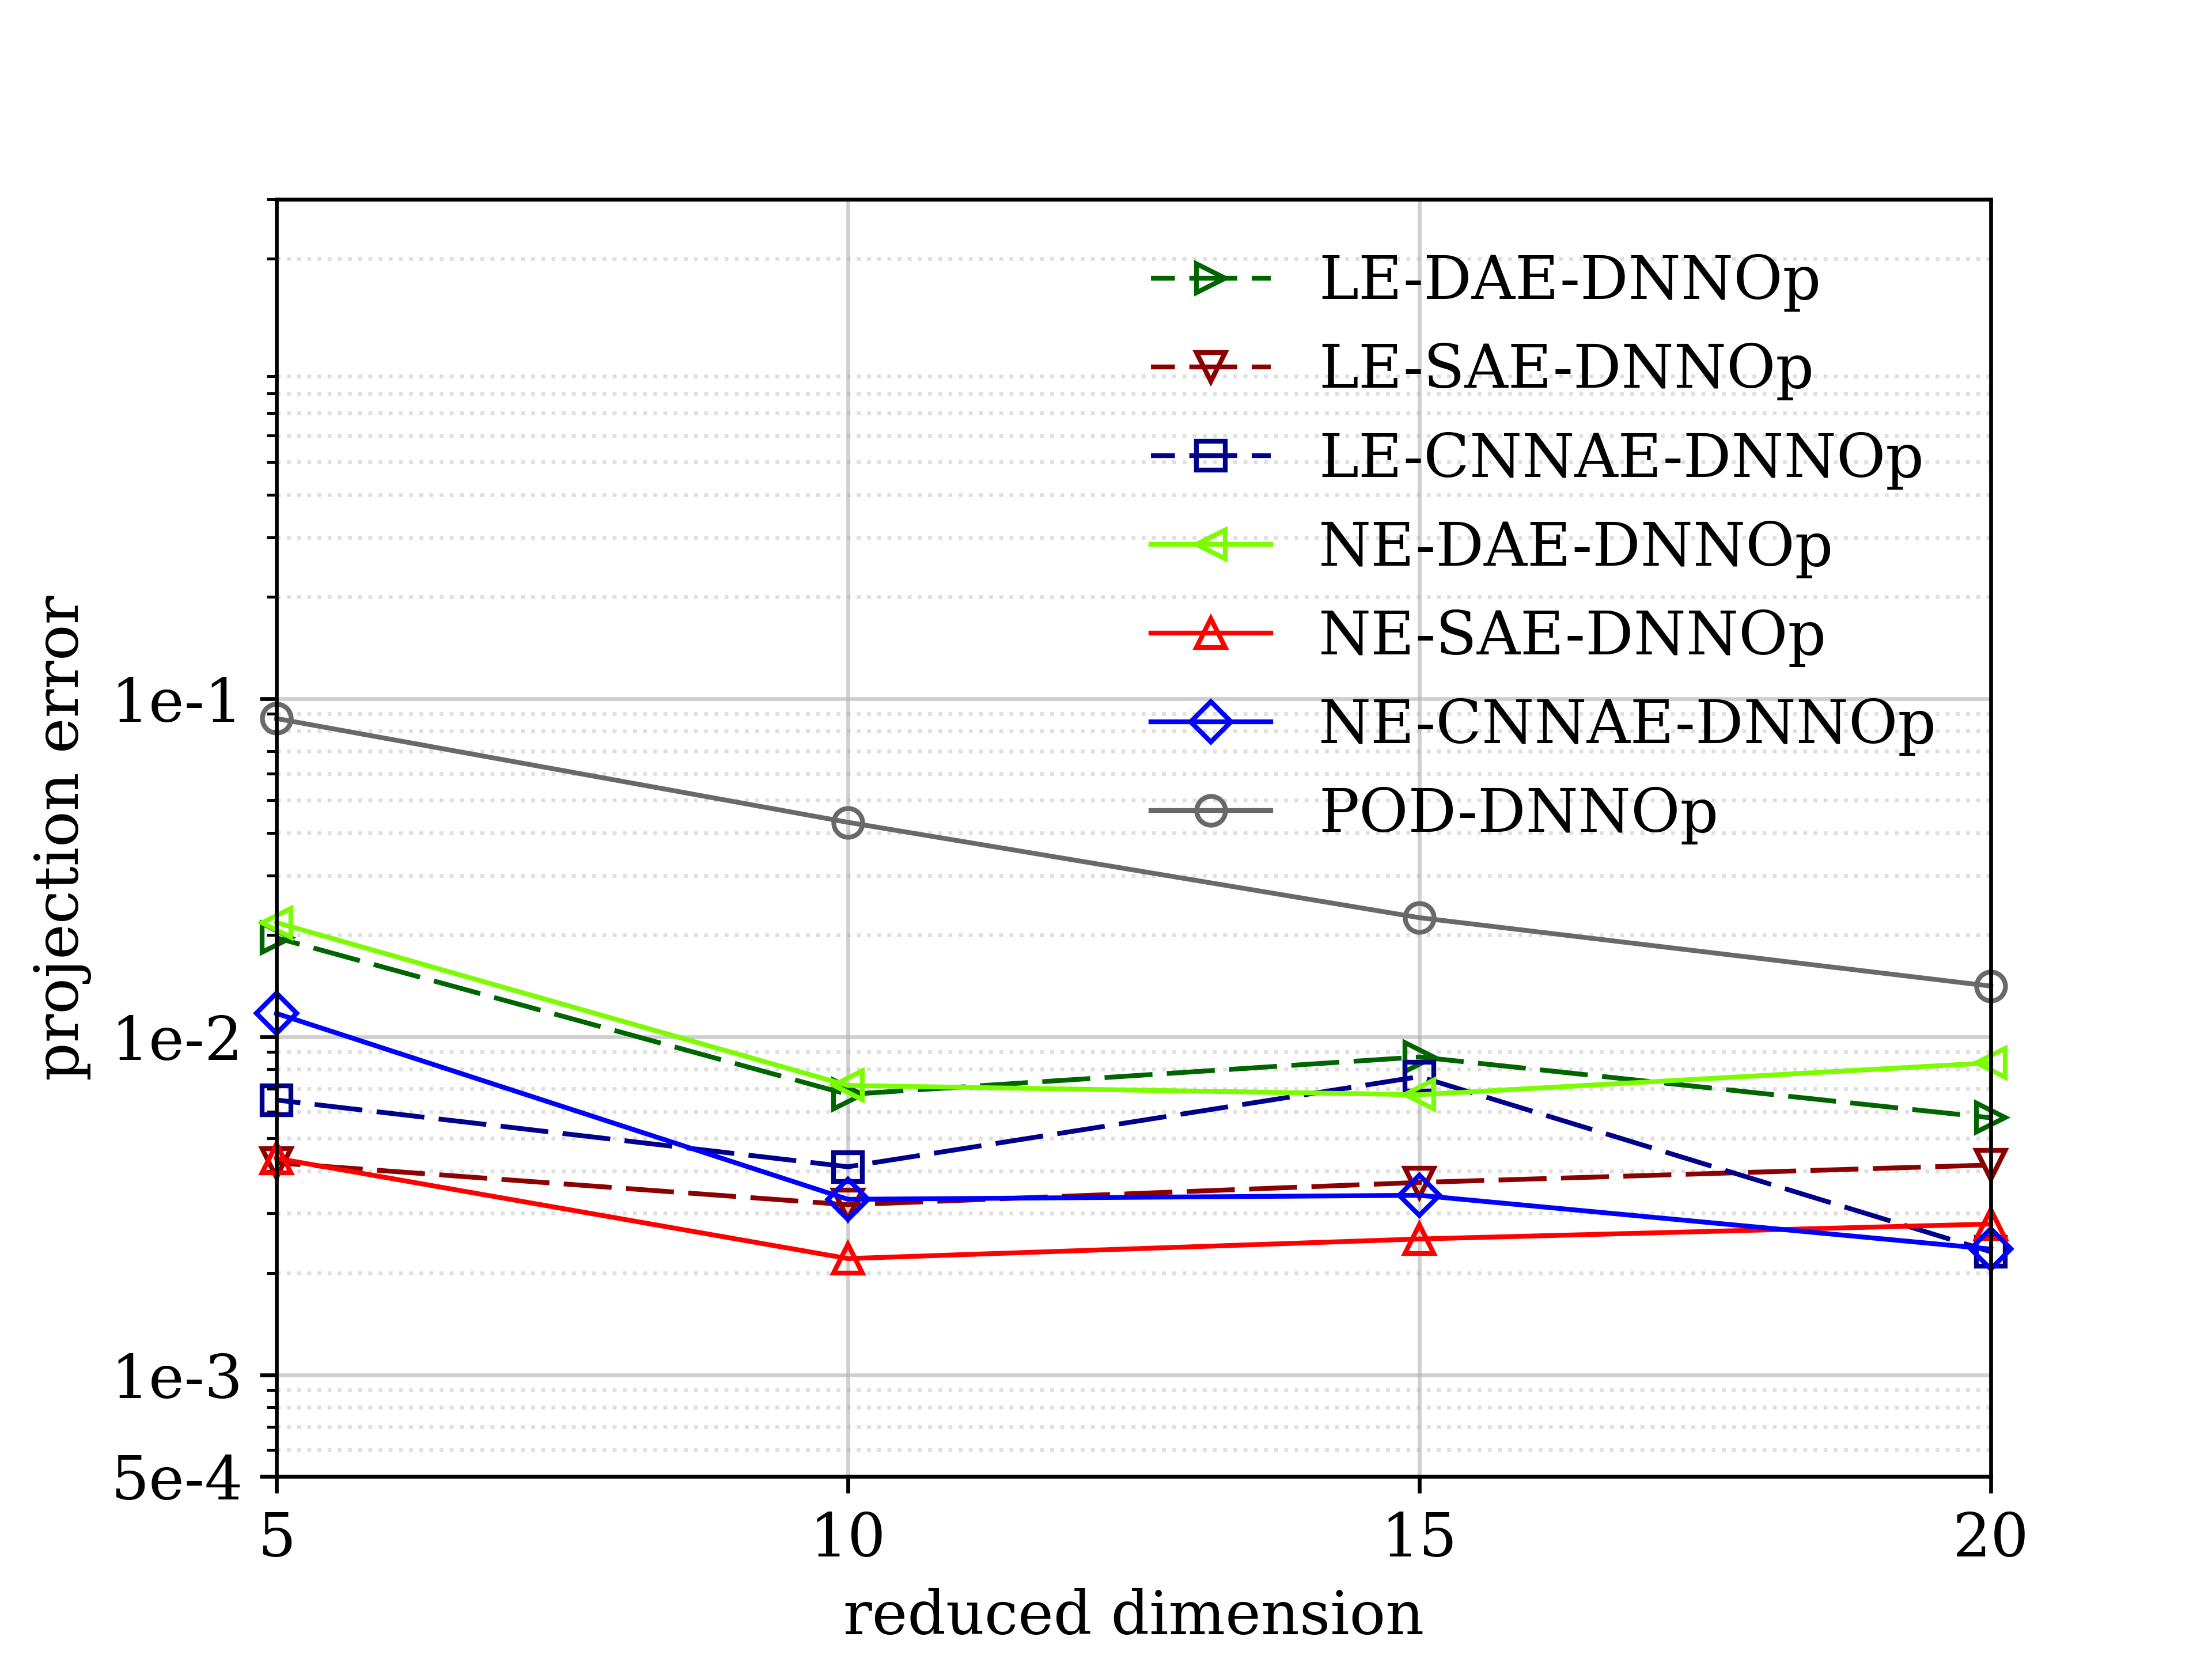
\includegraphics[width=\textwidth]{proj_err_rom_validation.png}
            \end{center}
            \caption{}
        \end{subfigure}
     \end{center}
        \caption[Projection errors on the test data.]{(a) Projection error between the latent spaces obtained from the surrogate operator $\mathcal{H}$; and (b) projection error of the reduced order model solution on the test dataset with $\mu = 1.0$ over different latent space dimension.}
        \label{fig: proj err rom solution}
\end{figure}
The projection error of the reduced-order model for the nonlinear autoencoders is lower than for the linear autoencoders. We summarized ROM solution and their absolute errors of the POD method in Fig.~\ref{fig: pod-burger} for four latent space dimensions. 

\begin{figure}[!htb]
     \begin{center}
        \begin{subfigure}[b]{0.23\textwidth}
            \begin{center}
                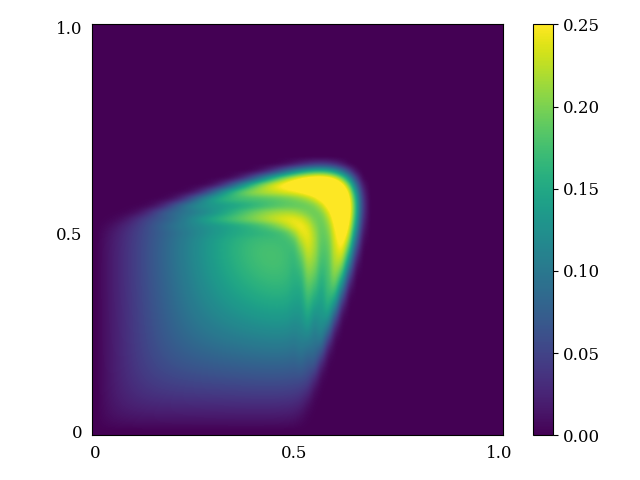
\includegraphics[trim = {0, 0, 3cm, 0}, clip, width=\textwidth]{X-rom-POD-5.png}
            \end{center}
            \caption{Solution $r = 5$}
        \end{subfigure}
   \begin{subfigure}[b]{0.23\textwidth}
            \begin{center}
       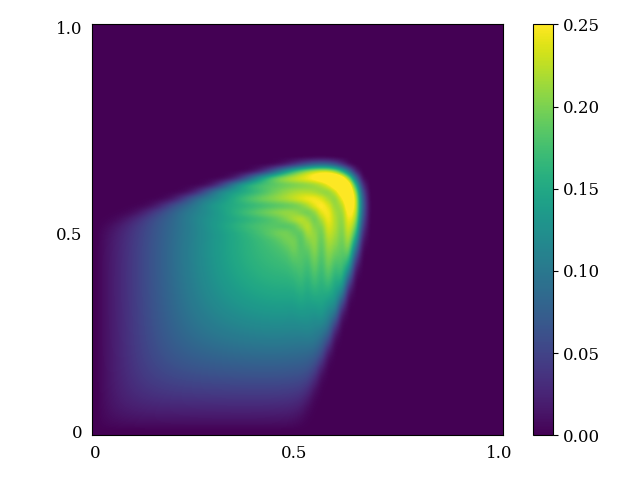
\includegraphics[trim = {0, 0, 3cm, 0}, clip, width=\textwidth]{X-rom-POD-10.png}
            \end{center}
            \caption{Solution $r = 10$}
        \end{subfigure}
   \begin{subfigure}[b]{0.23\textwidth}
            \begin{center}
       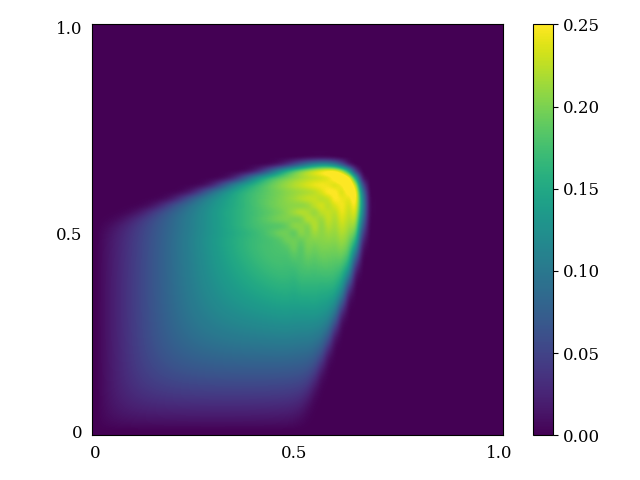
\includegraphics[trim = {0, 0, 3cm, 0}, clip, width=\textwidth]{X-rom-POD-15.png}
            \end{center}
            \caption{Solution $r = 15$}
        \end{subfigure}
   \begin{subfigure}[b]{0.23\textwidth}
       \begin{center}
        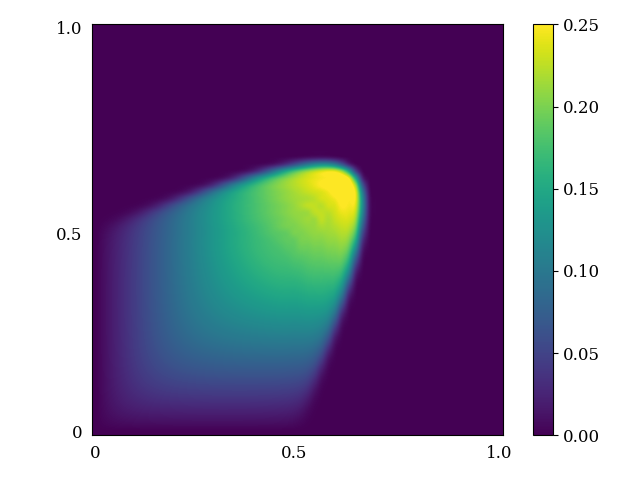
\includegraphics[trim = {0, 0, 3cm, 0}, clip, width=\textwidth]{X-rom-POD-20.png}
       \end{center}
       \caption{Solution $r = 20$}
        \end{subfigure}\\  
        \begin{subfigure}[b]{0.23\textwidth}
            \begin{center}
                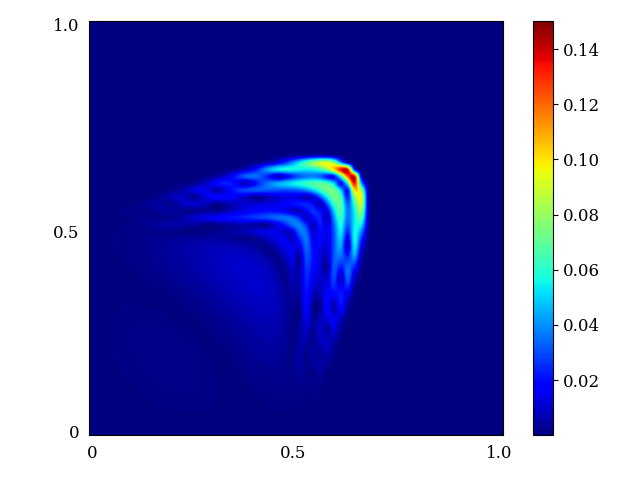
\includegraphics[trim = {0, 0, 3cm, 0}, clip, width=\textwidth]{X-rom-POD-5-abs-err.png}
            \end{center}
            \caption{Absolute error $r = 5$}
        \end{subfigure}  
        \begin{subfigure}[b]{0.23\textwidth}
            \begin{center}
                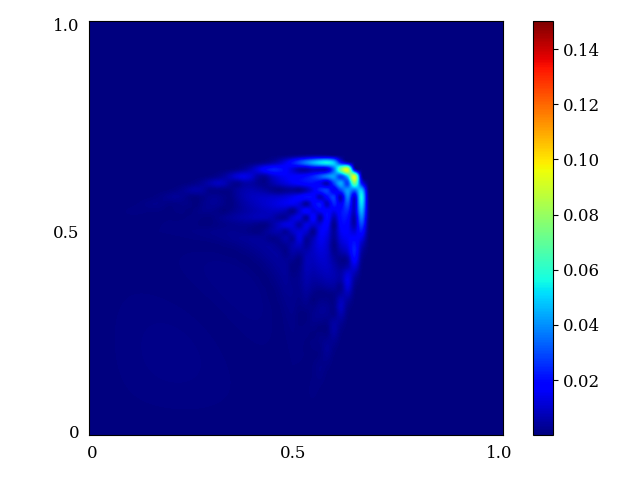
\includegraphics[trim = {0, 0, 3cm, 0}, clip, width=\textwidth]{X-rom-POD-10-abs-err.png}
            \end{center}
            \caption{Absolute error $r = 10$}
        \end{subfigure}   
        \begin{subfigure}[b]{0.23\textwidth}
            \begin{center}
                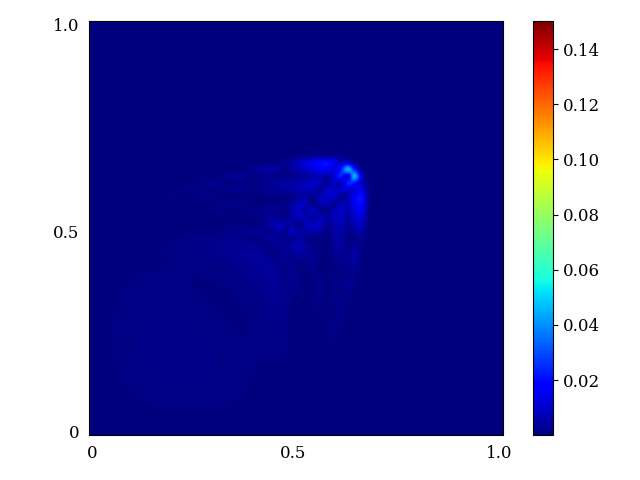
\includegraphics[trim = {0, 0, 3cm, 0}, clip, width=\textwidth]{X-rom-POD-15-abs-err.png}
            \end{center}
            \caption{Absolute error $r = 15$}
        \end{subfigure}    
        \begin{subfigure}[b]{0.23\textwidth}
            \begin{center}
                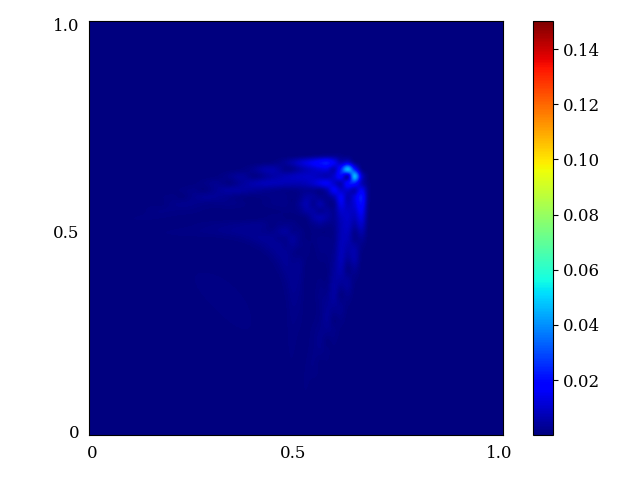
\includegraphics[trim = {0, 0, 3cm, 0}, clip, width=\textwidth]{X-rom-POD-20-abs-err.png}
            \end{center}
            \caption{Absolute error $r = 20$}
        \end{subfigure}
     \end{center}
     \caption[Solutions and pointwise errors for POD-DNNOp.]{Solutions (a, b, c, d) and pointwise errors (e, f, g, h) for POD-DNNOp with different latent space dimensions.}
        \label{fig: pod-burger}
\end{figure}
Both NE-SAE and NE-CNNAE have a projection error around $2\times10^{-3}$ and deliver the most accurate predictions. Their ROM solutions and associated absolute errors are shown in Fig.~\ref{fig: nesae-burger} and Fig.~\ref{fig: necnnae-burger}. 

\begin{figure}[!htb]
     \begin{center}
        \begin{subfigure}[b]{0.23\textwidth}
          \begin{center}
            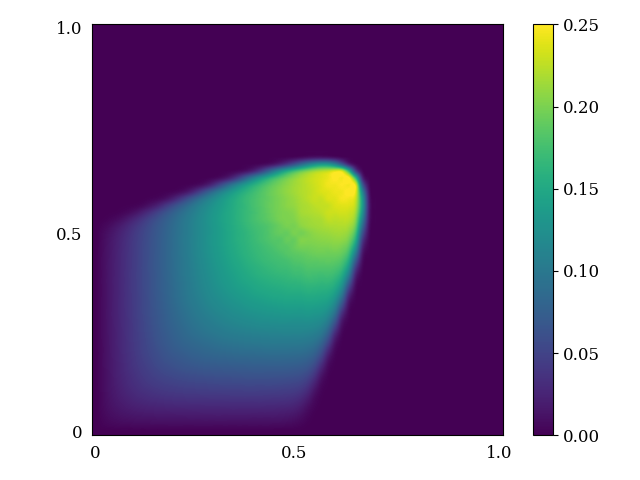
\includegraphics[trim = {0, 0, 3cm, 0}, clip, width=\textwidth]{X-rom-NE-SAE-5.png}
          \end{center}
            \caption{Solution $r = 5$}
        \end{subfigure}
   \begin{subfigure}[b]{0.23\textwidth}
       \begin{center}
        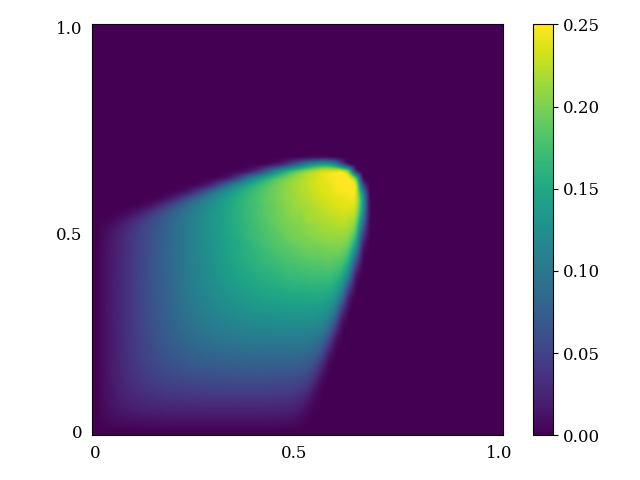
\includegraphics[trim = {0, 0, 3cm, 0}, clip, width=\textwidth]{X-rom-NE-SAE-10.png}
       \end{center}
            \caption{Solution $r = 10$}
        \end{subfigure}
   \begin{subfigure}[b]{0.23\textwidth}
            \begin{center}
                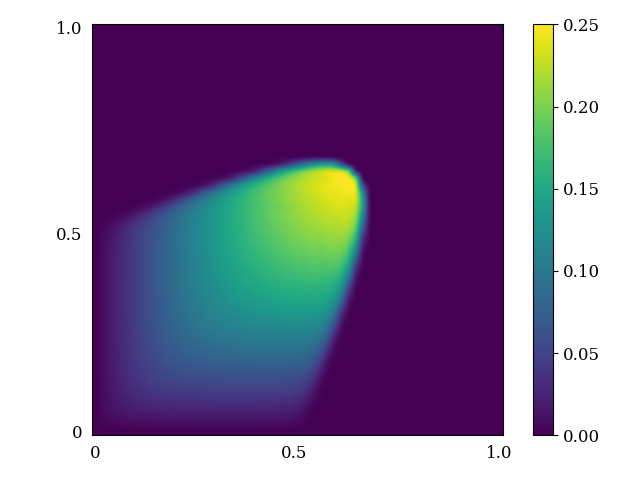
\includegraphics[trim = {0, 0, 3cm, 0}, clip, width=\textwidth]{X-rom-NE-SAE-15.png}
            \end{center}
            \caption{Solution $r = 15$}
        \end{subfigure}
   \begin{subfigure}[b]{0.23\textwidth}
            \begin{center}
                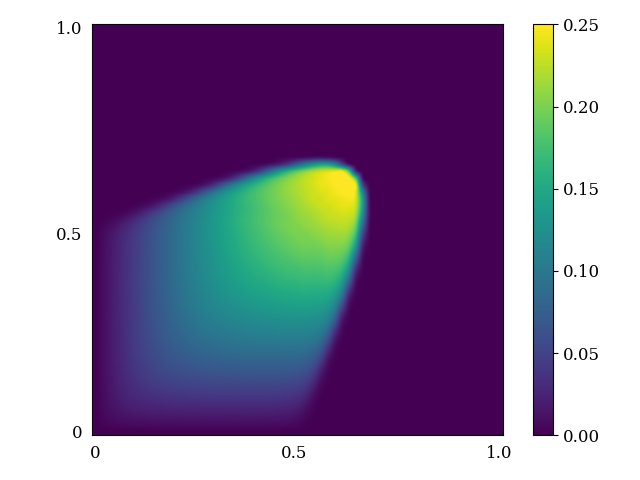
\includegraphics[trim = {0, 0, 3cm, 0}, clip, width=\textwidth]{X-rom-NE-SAE-20.png}
            \end{center}
            \caption{Solution $r = 20$}
        \end{subfigure}\\  
        \begin{subfigure}[b]{0.23\textwidth}
            \begin{center}
                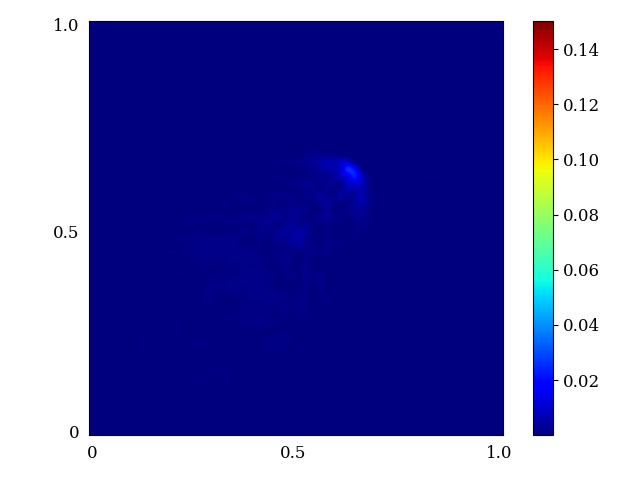
\includegraphics[trim = {0, 0, 3cm, 0}, clip, width=\textwidth]{X-rom-NE-SAE-5-abs-err.png}
            \end{center}
            \caption{Absolute error $r = 5$}
        \end{subfigure}  
        \begin{subfigure}[b]{0.23\textwidth}
            \begin{center}
                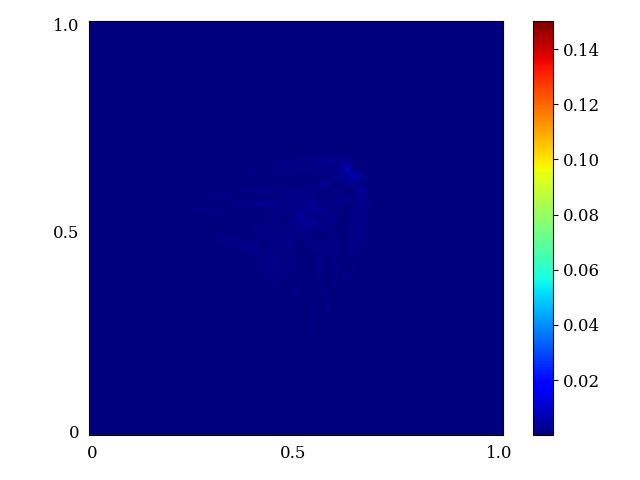
\includegraphics[trim = {0, 0, 3cm, 0}, clip, width=\textwidth]{X-rom-NE-SAE-10-abs-err.png}
            \end{center}
            \caption{Absolute error $r = 10$}
        \end{subfigure}   
        \begin{subfigure}[b]{0.23\textwidth}
            \begin{center}
                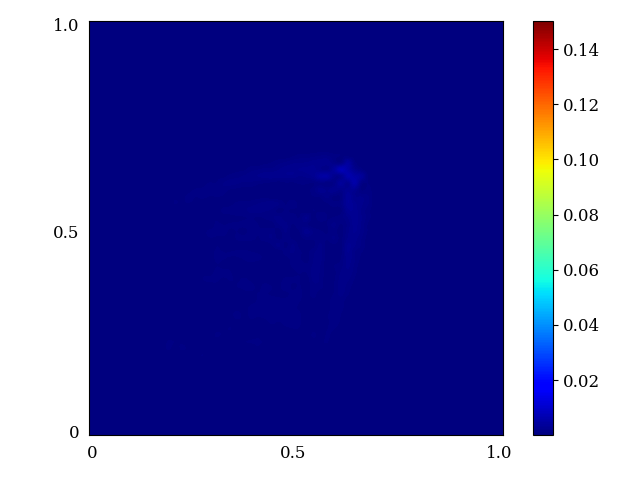
\includegraphics[trim = {0, 0, 3cm, 0}, clip, width=\textwidth]{X-rom-NE-SAE-15-abs-err.png}
            \end{center}
            \caption{Absolute error $r = 15$}
        \end{subfigure}    
        \begin{subfigure}[b]{0.23\textwidth}
            \begin{center}
                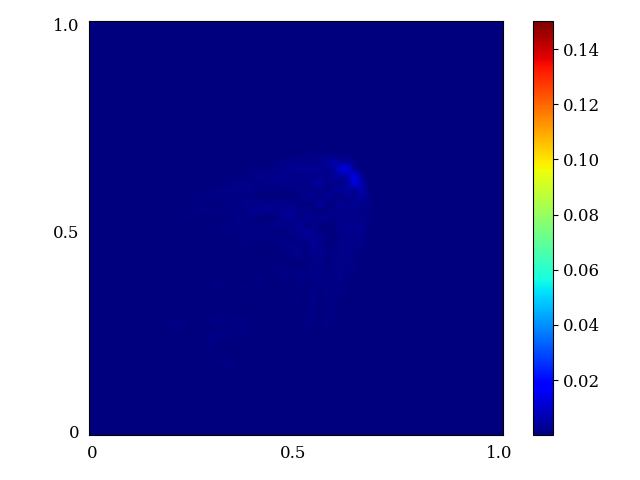
\includegraphics[trim = {0, 0, 3cm, 0}, clip, width=\textwidth]{X-rom-NE-SAE-20-abs-err.png}
            \end{center}
            \caption{Absolute error $r = 20$}
        \end{subfigure}
     \end{center}
     \caption[Solutions and pointwise errors for NE-SAE-DNNOp.]{Solutions (a, b, c, d) and pointwise errors (e, f, g, h) for NE-SAE-DNNOp with different latent space dimensions.}
        \label{fig: nesae-burger}
\end{figure}

\begin{figure}[!htb]
     \begin{center}
        \begin{subfigure}[b]{0.23\textwidth}
            \begin{center}
                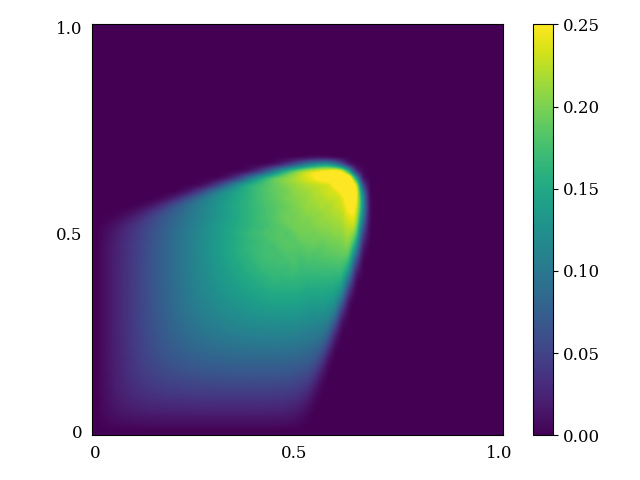
\includegraphics[trim = {0, 0, 3cm, 0}, clip, width=\textwidth]{X-rom-NE-CNNAE-5.png}
            \end{center}
            \caption{Solution $r = 5$}
        \end{subfigure}
   \begin{subfigure}[b]{0.23\textwidth}
            \begin{center}
                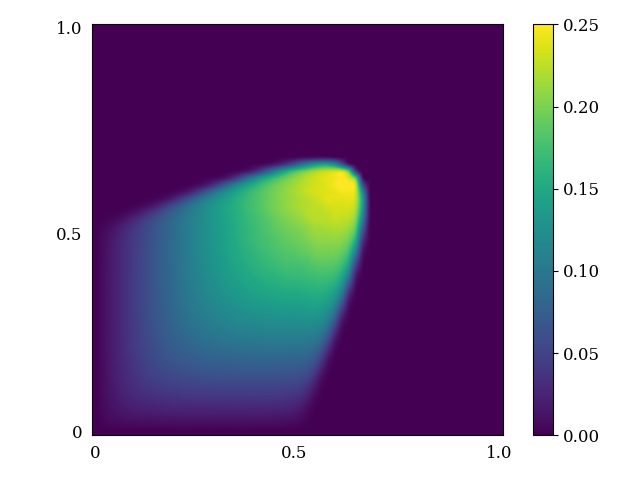
\includegraphics[trim = {0, 0, 3cm, 0}, clip, width=\textwidth]{X-rom-NE-CNNAE-10.png}
            \end{center}
            \caption{Solution $r = 10$}
        \end{subfigure}
   \begin{subfigure}[b]{0.23\textwidth}
            \begin{center}
                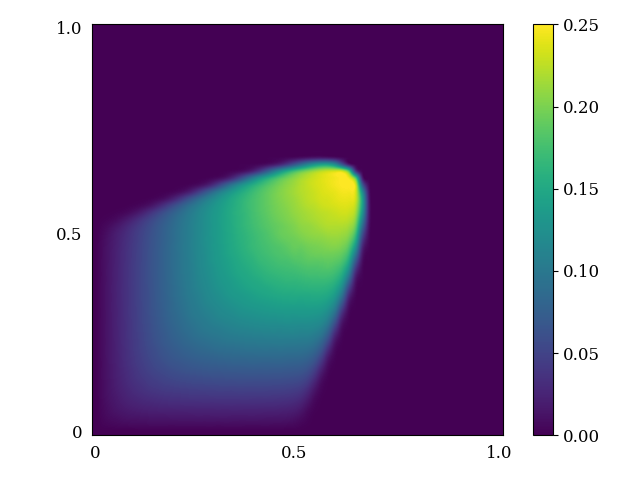
\includegraphics[trim = {0, 0, 3cm, 0}, clip, width=\textwidth]{X-rom-NE-CNNAE-15.png}
            \end{center}
            \caption{Solution $r = 15$}
        \end{subfigure}
   \begin{subfigure}[b]{0.23\textwidth}
           \begin{center}
            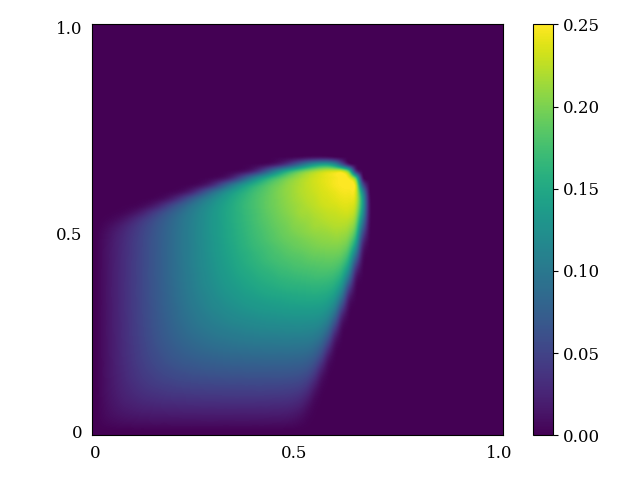
\includegraphics[trim = {0, 0, 3cm, 0}, clip, width=\textwidth]{X-rom-NE-CNNAE-20.png}
           \end{center}
            \caption{Solution $r = 20$}
        \end{subfigure}\\  
        \begin{subfigure}[b]{0.23\textwidth}
            \begin{center}
                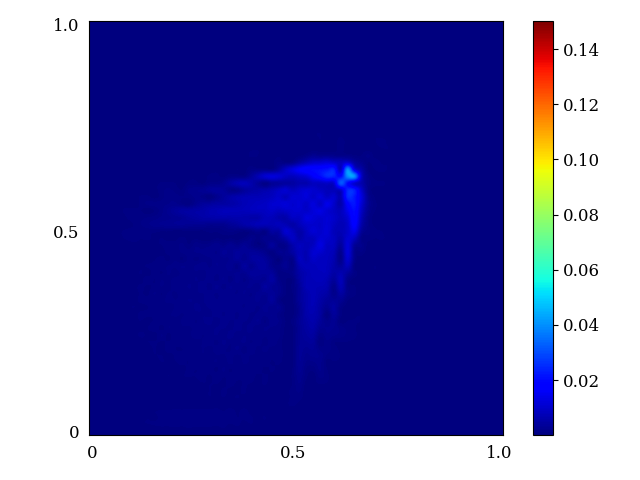
\includegraphics[trim = {0, 0, 3cm, 0}, clip, width=\textwidth]{X-rom-NE-CNNAE-5-abs-err.png}
            \end{center}
            \caption{Absolute error $r = 5$}
        \end{subfigure}  
        \begin{subfigure}[b]{0.23\textwidth}
            \begin{center}
                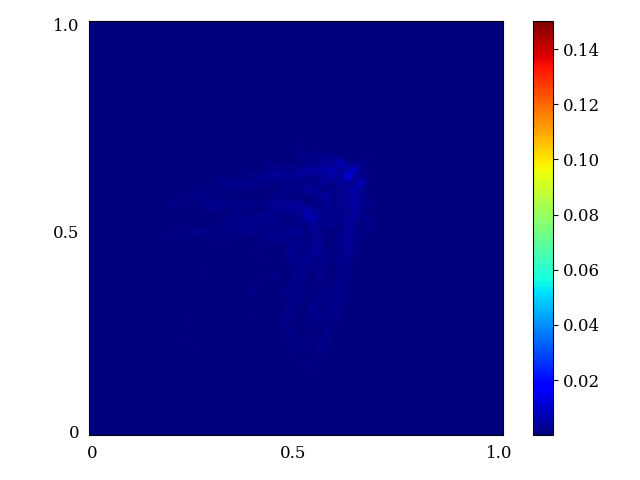
\includegraphics[trim = {0, 0, 3cm, 0}, clip, width=\textwidth]{X-rom-NE-CNNAE-10-abs-err.png}
            \end{center}
            \caption{Absolute error $r = 10$}
        \end{subfigure}   
        \begin{subfigure}[b]{0.23\textwidth}
            \begin{center}
                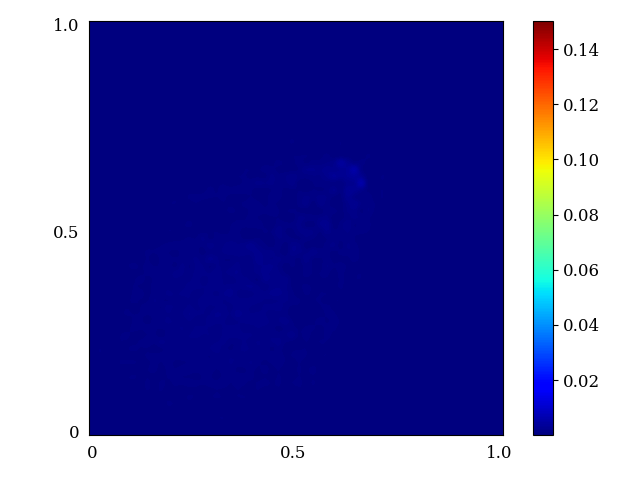
\includegraphics[trim = {0, 0, 3cm, 0}, clip, width=\textwidth]{X-rom-NE-CNNAE-15-abs-err.png}
            \end{center}
            \caption{Absolute error $r = 15$}
        \end{subfigure}    
        \begin{subfigure}[b]{0.23\textwidth}
            \begin{center}
                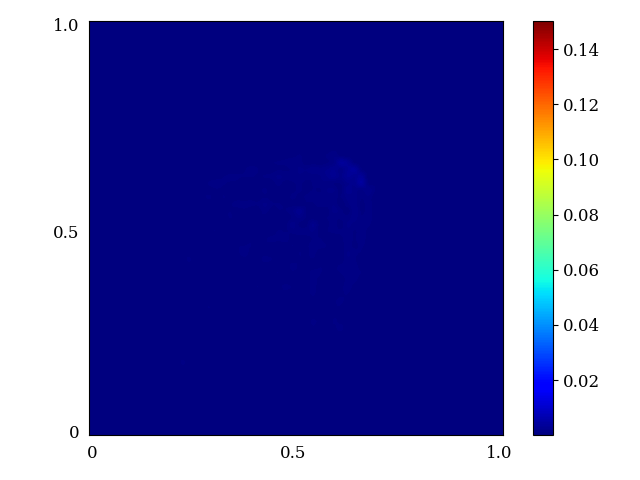
\includegraphics[trim = {0, 0, 3cm, 0}, clip, width=\textwidth]{X-rom-NE-CNNAE-20-abs-err.png}
            \end{center}
            \caption{Absolute error $r = 20$}
        \end{subfigure}
     \end{center}
     \caption[Solutions and pointwise errors for NE-CNNAE-DNNOp.]{Solutions (a, b, c, d) and pointwise errors (e, f, g, h) for NE-CNNAE-DNNOp with different latent space dimensions.}
        \label{fig: necnnae-burger}
\end{figure}

The absolute errors decrease together when latent dimension increases. However, oscillations in the ROM solution of the POD method can still be observed for $r = 20$. These oscillations can also be observed from the ROM solution with the LE-DAE and NE-DAE, but are not present for NE-CNNAE and NE-SAE when $r \in \{15, 20\}$.

The adaptivity in the bases promoted in the CNNAE approach is illustrated in Fig.~\ref{fig:adaptivity}, which shows how one particular basis (here, $D_4$) evolves as a function of time (similar responses are obtained for the other bases).
\begin{figure}[!htb]
     \begin{center}
        \begin{subfigure}[b]{0.22\textwidth}
            \begin{center}
                \includegraphics[trim = {0, 0, 3cm, 0}, clip, width=\textwidth]{Figure_Base_3_Snapshot_2.pdf}
            \end{center}
            \caption{$M = 201$}
        \end{subfigure}
   \begin{subfigure}[b]{0.22\textwidth}
       \begin{center}
        \includegraphics[trim = {0, 0, 3cm, 0}, clip, width=\textwidth]{Figure_Base_3_Snapshot_6.pdf}
       \end{center}
            \caption{$M = 601$}
        \end{subfigure}
   \begin{subfigure}[b]{0.22\textwidth}
       \begin{center}
        \includegraphics[trim = {0, 0, 3cm, 0}, clip, width=\textwidth]{Figure_Base_3_Snapshot_10.pdf}
       \end{center}
            \caption{$M = 1001$}
        \end{subfigure}
   \begin{subfigure}[b]{0.26\textwidth}
       \begin{center}
        \includegraphics[trim = {0, 0, 0cm, 0}, clip, width=\textwidth]{Figure_Base_3_Snapshot_14.pdf}
       \end{center}
            \caption{$M = 1401$}
        \end{subfigure}
     \end{center}
\caption[Evolution of the fourth basis in CNNAE.]{This figure illustrates adaptivity by showing the evolution of the fourth basis in Eq.~\eqref{eq: cnn decoder}. Here, we take the basis at the 101st time step as reference, and plot the evolution of the difference $\Delta D_4(M) = D_4(\hat{u}_4^{\left<M\right>}; \hat{\btu}^{\left<M\right>}) - D_4(\hat{u}_4^{\left<101\right>}; \hat{\btu}^{\left<101\right>})$ at selected time steps (namely, 201, 601, 1001, and 1401). Note that the basis is shown in physical space to enable proper visualization.}
\label{fig:adaptivity}
\end{figure}
This adaptivity mechanism helps capture the features exhibited by the solution as the simulation progresses, hence facilitating interpretation.

The performance of vectorized implicit time integration was assessed by measuring the  computational cost of flow map estimation for 1500 time steps, using wall-clock time and multiple GPUs --- as speed up also varies based on the hardware itself. The timing is obtained by performing calculations on NVIDIA RTX A4500 (64 bits, 33MHz, 20 GB), and NVIDIA RTX A6000 (64 bits, 33MHz, 48 GB), NVIDIA GeForce 4080 (64 bits, 33MHz, 16 GB). The wall-clock times are provided in Tab.~\ref{Tab:A4500}. The algorithm improves performance for $r \geq 15$, regardless of chunk size, with a maximum speed-up of 25.48 when solving the reduced order model in the latent space (as compared to serial solving for the ROM). Observe that $r \geq 15$, speed-ups do not decrease as the chunk size reaches 100. This implies that memory limitation (hardware limitation) was not reached for any of the GPUs, which indicates that the tested chunk sizes may be suboptimal. For $r = 10$ and a chunk size equal to 100, speed-ups decrease for all configurations, which suggests that for this specific case, the required number of nonlinear iterations is larger than for the other cases. For this choice of parameters, the solver eventually fails, hence resulting in infinite projection errors (as shown in Tab.~\ref{Tab:A4500}). To further support this explanation, the maximum number of Newton-Raphson (N-R) iterations required for each chunk when solving the adjoint integration problems is also reported. It is seen that when $r = 10$ and for a chunk size equal to 100, the number of nonlinear iterations reaches its maximum allowed value (set to 100), for all GPUs. This behavior is a manifestation of the interplay between the chunk size, the initial guess in the Newton-Raphson solver, and the latent space dimension. When the dimension $r$ are large enough, the solution can be obtained even under poor initialization: the number of solver iterations then increases together with the chunk size. This can be seen in Tab.~\ref{Tab:A4500}: when the chunk size equals 1, around 2 iterations are necessary to reach convergence, while around 10 iterations are needed for a chunk size set to 100.
\begin{table}[!ht]
    \caption[Wall-clock times on multiple GPUs.]{Wall-clock times at different latent space dimensions and chunk size on NVIDIA RTX A4500, NVIDIA RTX A6000, and NVIDIA GeForce 4080 for 1500 time steps on the test dataset ($\mu = 1.0$). The shortest wall-clock time is obtained when $r = 15$ using NVIDIA RTX A6000 with 1.32 seconds.}
    \label{Tab:A4500}
    \begin{center}
        \small
    \begin{tabular}{|c|c|c|c|c|c|c|c|c|c|c|c|c|}
    \hline
    \multicolumn{13}{|c|}{NVIDIA RTX A4500} \\ \cline{1-13}
    Reduced dimension $r$ & \multicolumn{4}{|c|}{10} & \multicolumn{4}{|c|}{15} & \multicolumn{4}{|c|}{20}\\ \hline
    Chunk size & 1 & 10 & 50 & 100 & 1 & 10 & 50 & 100 & 1 & 10 & 50 & 100 \\ \hline
    Projection error (\%) & 0.33 & 0.33 & 0.33 & INF & 0.34 & 0.34 & 0.34 & 0.34 & 0.23 & 0.23 & 0.23 & 0.23 \\ \hline
    N-R iterations $\#$ & 2 & 3 & 6 & 100 & 3 & 3 & 5 & 7 & 3 & 4 & 7 & 12 \\ \hline
    Wall time (sec) & 34.08 & 5.10 & 1.61 & 6.94 & 34.65 & 5.06 & 1.62 & 1.36 & 34.46 & 5.07 & 1.78 & 1.48 \\ \hline 
    Speed-up & 1 & 6.68 & 21.17 & 4.91 & 1 & 6.85 & 21.39 & \textbf{25.48} & 1 & 6.80 & 19.36 & 23.28 \\ \hline
    \multicolumn{13}{|c|}{NVIDIA RTX A6000} \\ \cline{1-13}
    Reduced dimension $r$ &\multicolumn{4}{|c|}{10} & \multicolumn{4}{|c|}{15} & \multicolumn{4}{|c|}{20}\\ \hline
    Chunk size & 1 & 10 & 50 & 100 & 1 & 10 & 50 & 100 & 1 & 10 & 50 & 100 \\ \hline
    Projection error (\%) & 0.33 & 0.33 & 0.33 & INF & 0.34 & 0.34 & 0.34 & 0.34 & 0.23 & 0.23 & 0.23 & 0.23 \\ \hline
    N-R iterations $\#$ & 2 & 3 & 6 & 100 & 3 & 3 & 5 & 6 & 2 & 3 & 6 & 8 \\ \hline 
    Wall time (sec) & 10.49 & 2.4 & 1.2 & 5.87 & 10.72 & 2.34 & 1.42 & \textbf{1.32} & 14.19 & 2.26 & 2.08 & 1.38 \\ \hline 
    Speed-up & 1 & 4.37 & 8.74 & 1.79 & 1 & 4.58 & 7.55 & 8.12 & 1 & 6.59 & 7.16 & 10.80 \\ \hline
    \multicolumn{13}{|c|}{NVIDIA GeForce 4080} \\ \cline{1-13}
    Reduced dimension $r$ & \multicolumn{4}{|c|}{10} & \multicolumn{4}{|c|}{15} & \multicolumn{4}{|c|}{20}\\ \hline
    Chunk size & 1 & 10 & 50 & 100 & 1 & 10 & 50 & 100 & 1 & 10 & 50 & 100 \\ \hline
    Projection error (\%) & 0.33 & 0.33 & 0.33 & INF & 0.34 & 0.34 & 0.34 & 0.34 & 0.23 & 0.23 & 0.23 & 0.23 \\ \hline
    N-R iterations $\#$ & 2 & 3 & 6 & 100 & 3 & 3 & 5 & 7 & 2 & 3 & 5 & 7 \\ \hline 
    Wall-clock time (sec) & 14.74 & 1.37 & 0.73 & 8.69 & 13.02 & 2.59 & 1.50 & 1.51 & 13.52 & 2.62 & 1.64 & 1.64 \\ \hline 
    Speed-up & 1 & 10.76 & 20.19 & 1.67 & 1 & 5.03 & 8.67 & 8.62 & 1 & 5.16 & 8.24 & 8.24 \\ \hline
    \end{tabular}
    \end{center}
 \end{table}

We also evaluated the performance of NE-CNNAE on other datasets beyond the range of the training dataset, for $\mu = 1.11$, $1.12$, $1.13$, $1.14$, $1.15$. The projection errors of the reduced-order model and the projection error between the latent spaces of NE-CNNAE with $n = 20$ are shown in Fig.~\ref{fig: extrapolate}. This figure illustrates how the accuracy decreases in the extrapolation regime, with an increase of almost one order of magnitude between $\mu = 1.1$ (included in the training dataset) and $\mu = 1.15$.

\begin{figure}[!htb]
     \begin{center}
        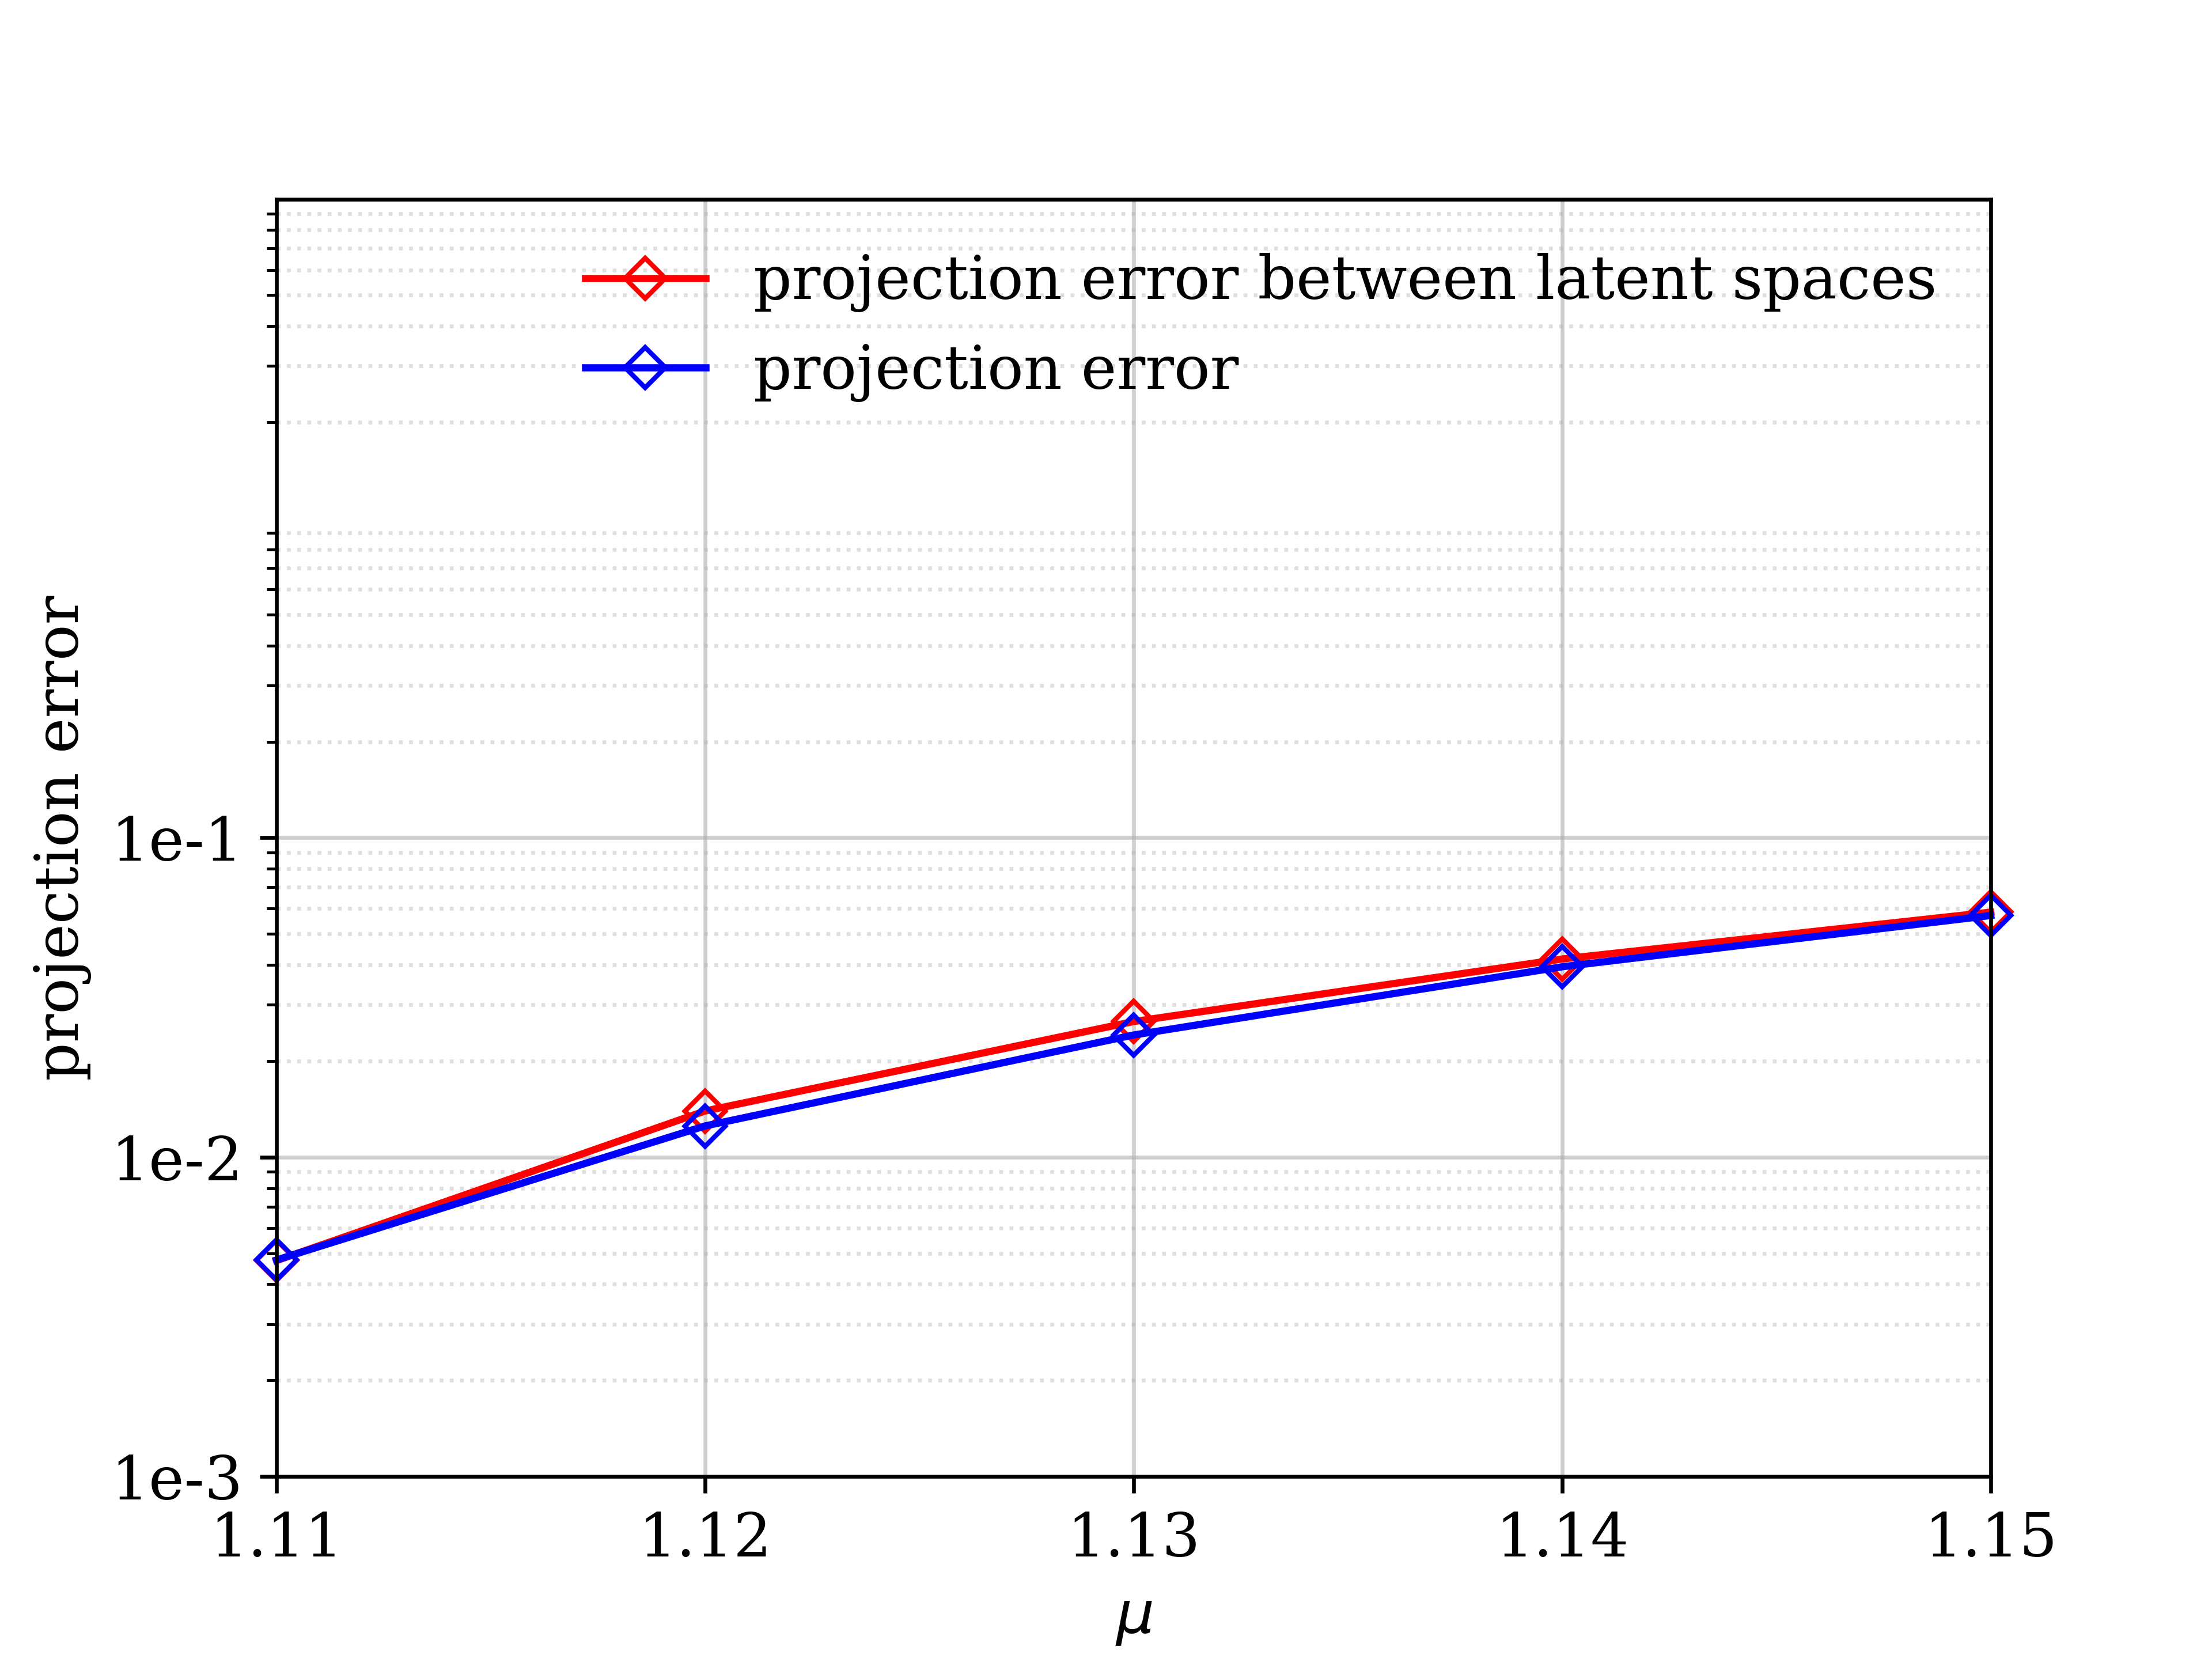
\includegraphics[width=0.49\textwidth]{extrapolate.png}
     \end{center}
     \caption[Projection error on extrapolated dataset.]{Projection error between the latent spaces obtained from the surrogate operator $\mathcal{H}$ and projection error of the reduced-order model solution on the test dataset with $\mu = 1.11$, $1.12$, $1.13$, $1.14$, $1.15$ when $n = 20$ of NE-CNNAE.}
        \label{fig: extrapolate}
\end{figure}


\subsection{Remarks on Complexity and Time Step Size Dependency}\label{subsec:time-dependency}

For nonlinear autoencoders, the number of trainable parameters can be considered as a measure of model complexity. For the above numerical example, with a latent dimension equal to 20, DAE has around 140 millions of trainable parameters, SAE has around 25 millions of trainable parameters, and the proposed CNNAE (which achieves best performance, together with SAE) has around 1 million trainable parameters. When training the models for 22 batches per epoch on NVIDIA RTX A4500 (64 bits, 33 MHz, 20 GB), with each batch containing approximately 246 time steps of solutions with a latent dimension set to 20, LE-DAE requires 14.70 seconds, LE-SAE 14.96 seconds, LE-CNNAE 1.56 seconds, NE-DAE 14.72 seconds, NE-SAE 14.98 seconds, and NE-CNNAE requires 1.58 seconds per epoch (average wall-clock time over 100 epochs).

It should be noticed that the considered operator learning strategies are, by construction, dependent on the time step size used for the training dataset. To quantify this effect, projection errors (in latent space and for the reduced-order model) obtained with NE-SAE and NE-CNNAE, and refined step sizes, are shown in Fig.~\ref{fig: time step size dependency}. Here, the surrogates were trained with a time step size denoted by $\Delta t$, and the projection errors are evaluated by running both the FOM and ROMs with decreasing time step sizes: $\{\Delta t, \Delta t / 2, \Delta t / 4, \Delta t / 8\}$.
\begin{figure}[!htb]
     \begin{center}
        \begin{subfigure}[b]{0.49\textwidth}
            \begin{center}
                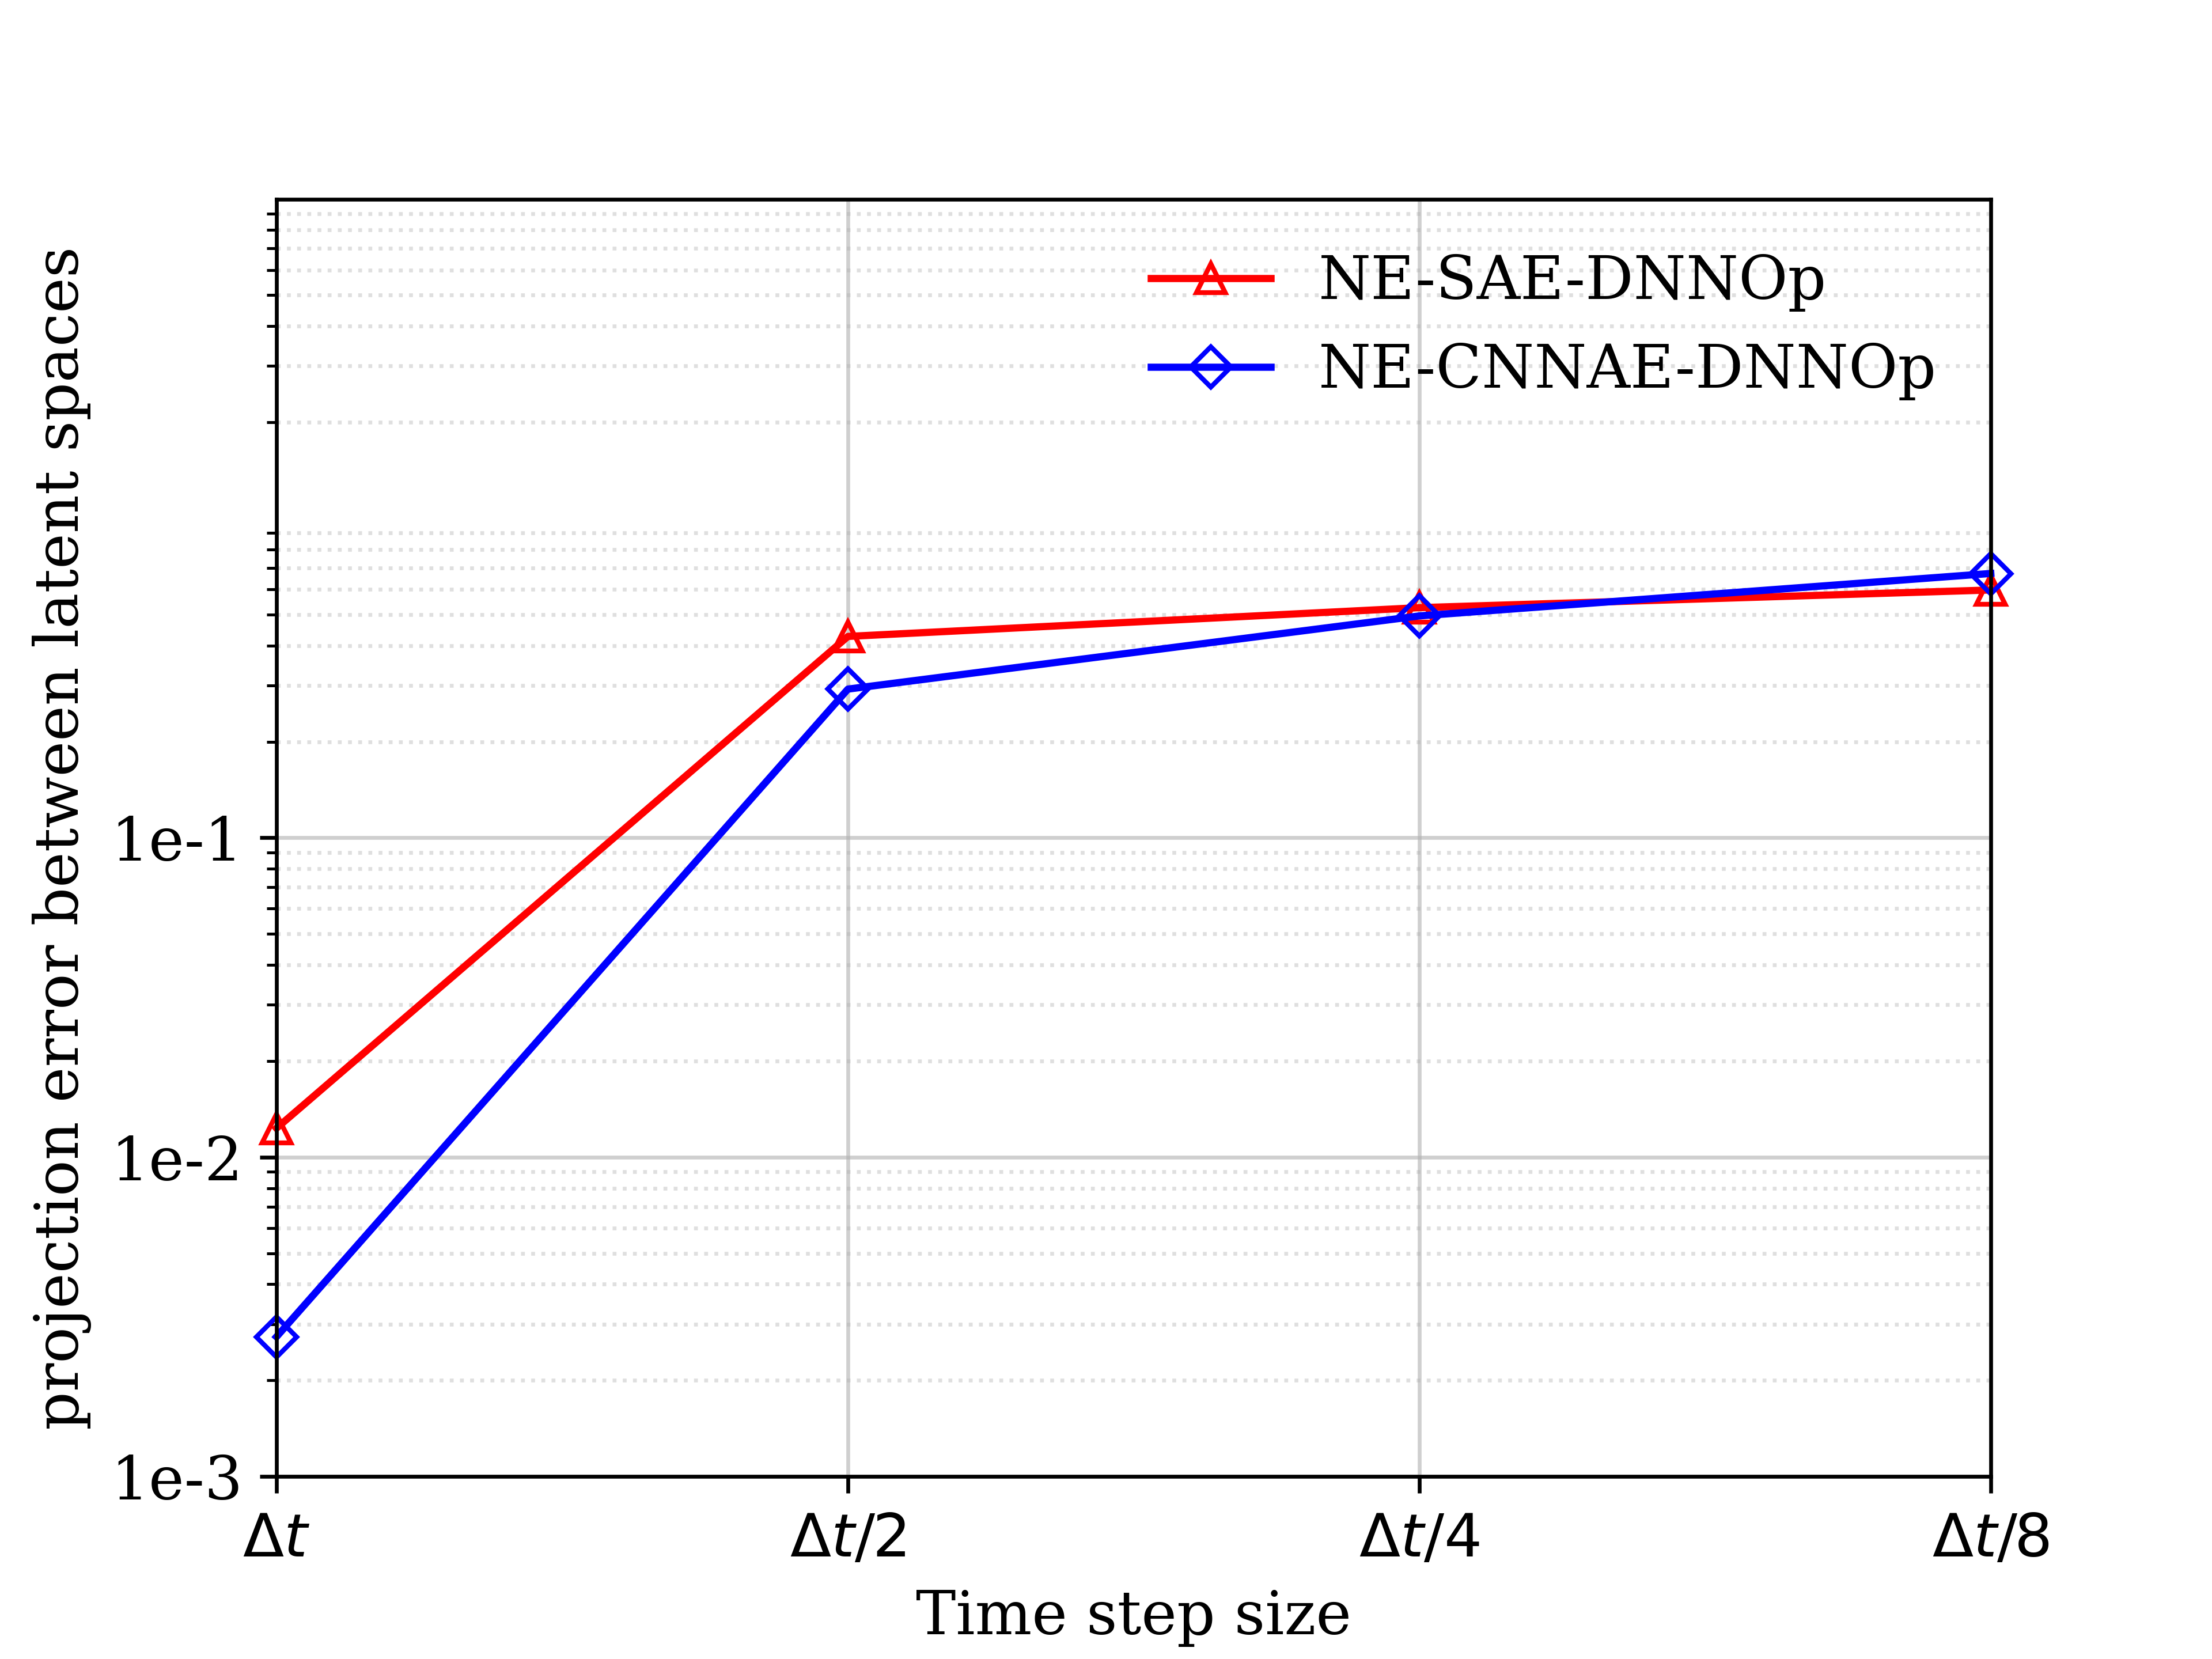
\includegraphics[width=\textwidth]{rom_hat_step_size.png}
            \end{center}
            \caption{}
        \end{subfigure}
        \begin{subfigure}[b]{0.49\textwidth}
            \begin{center}
                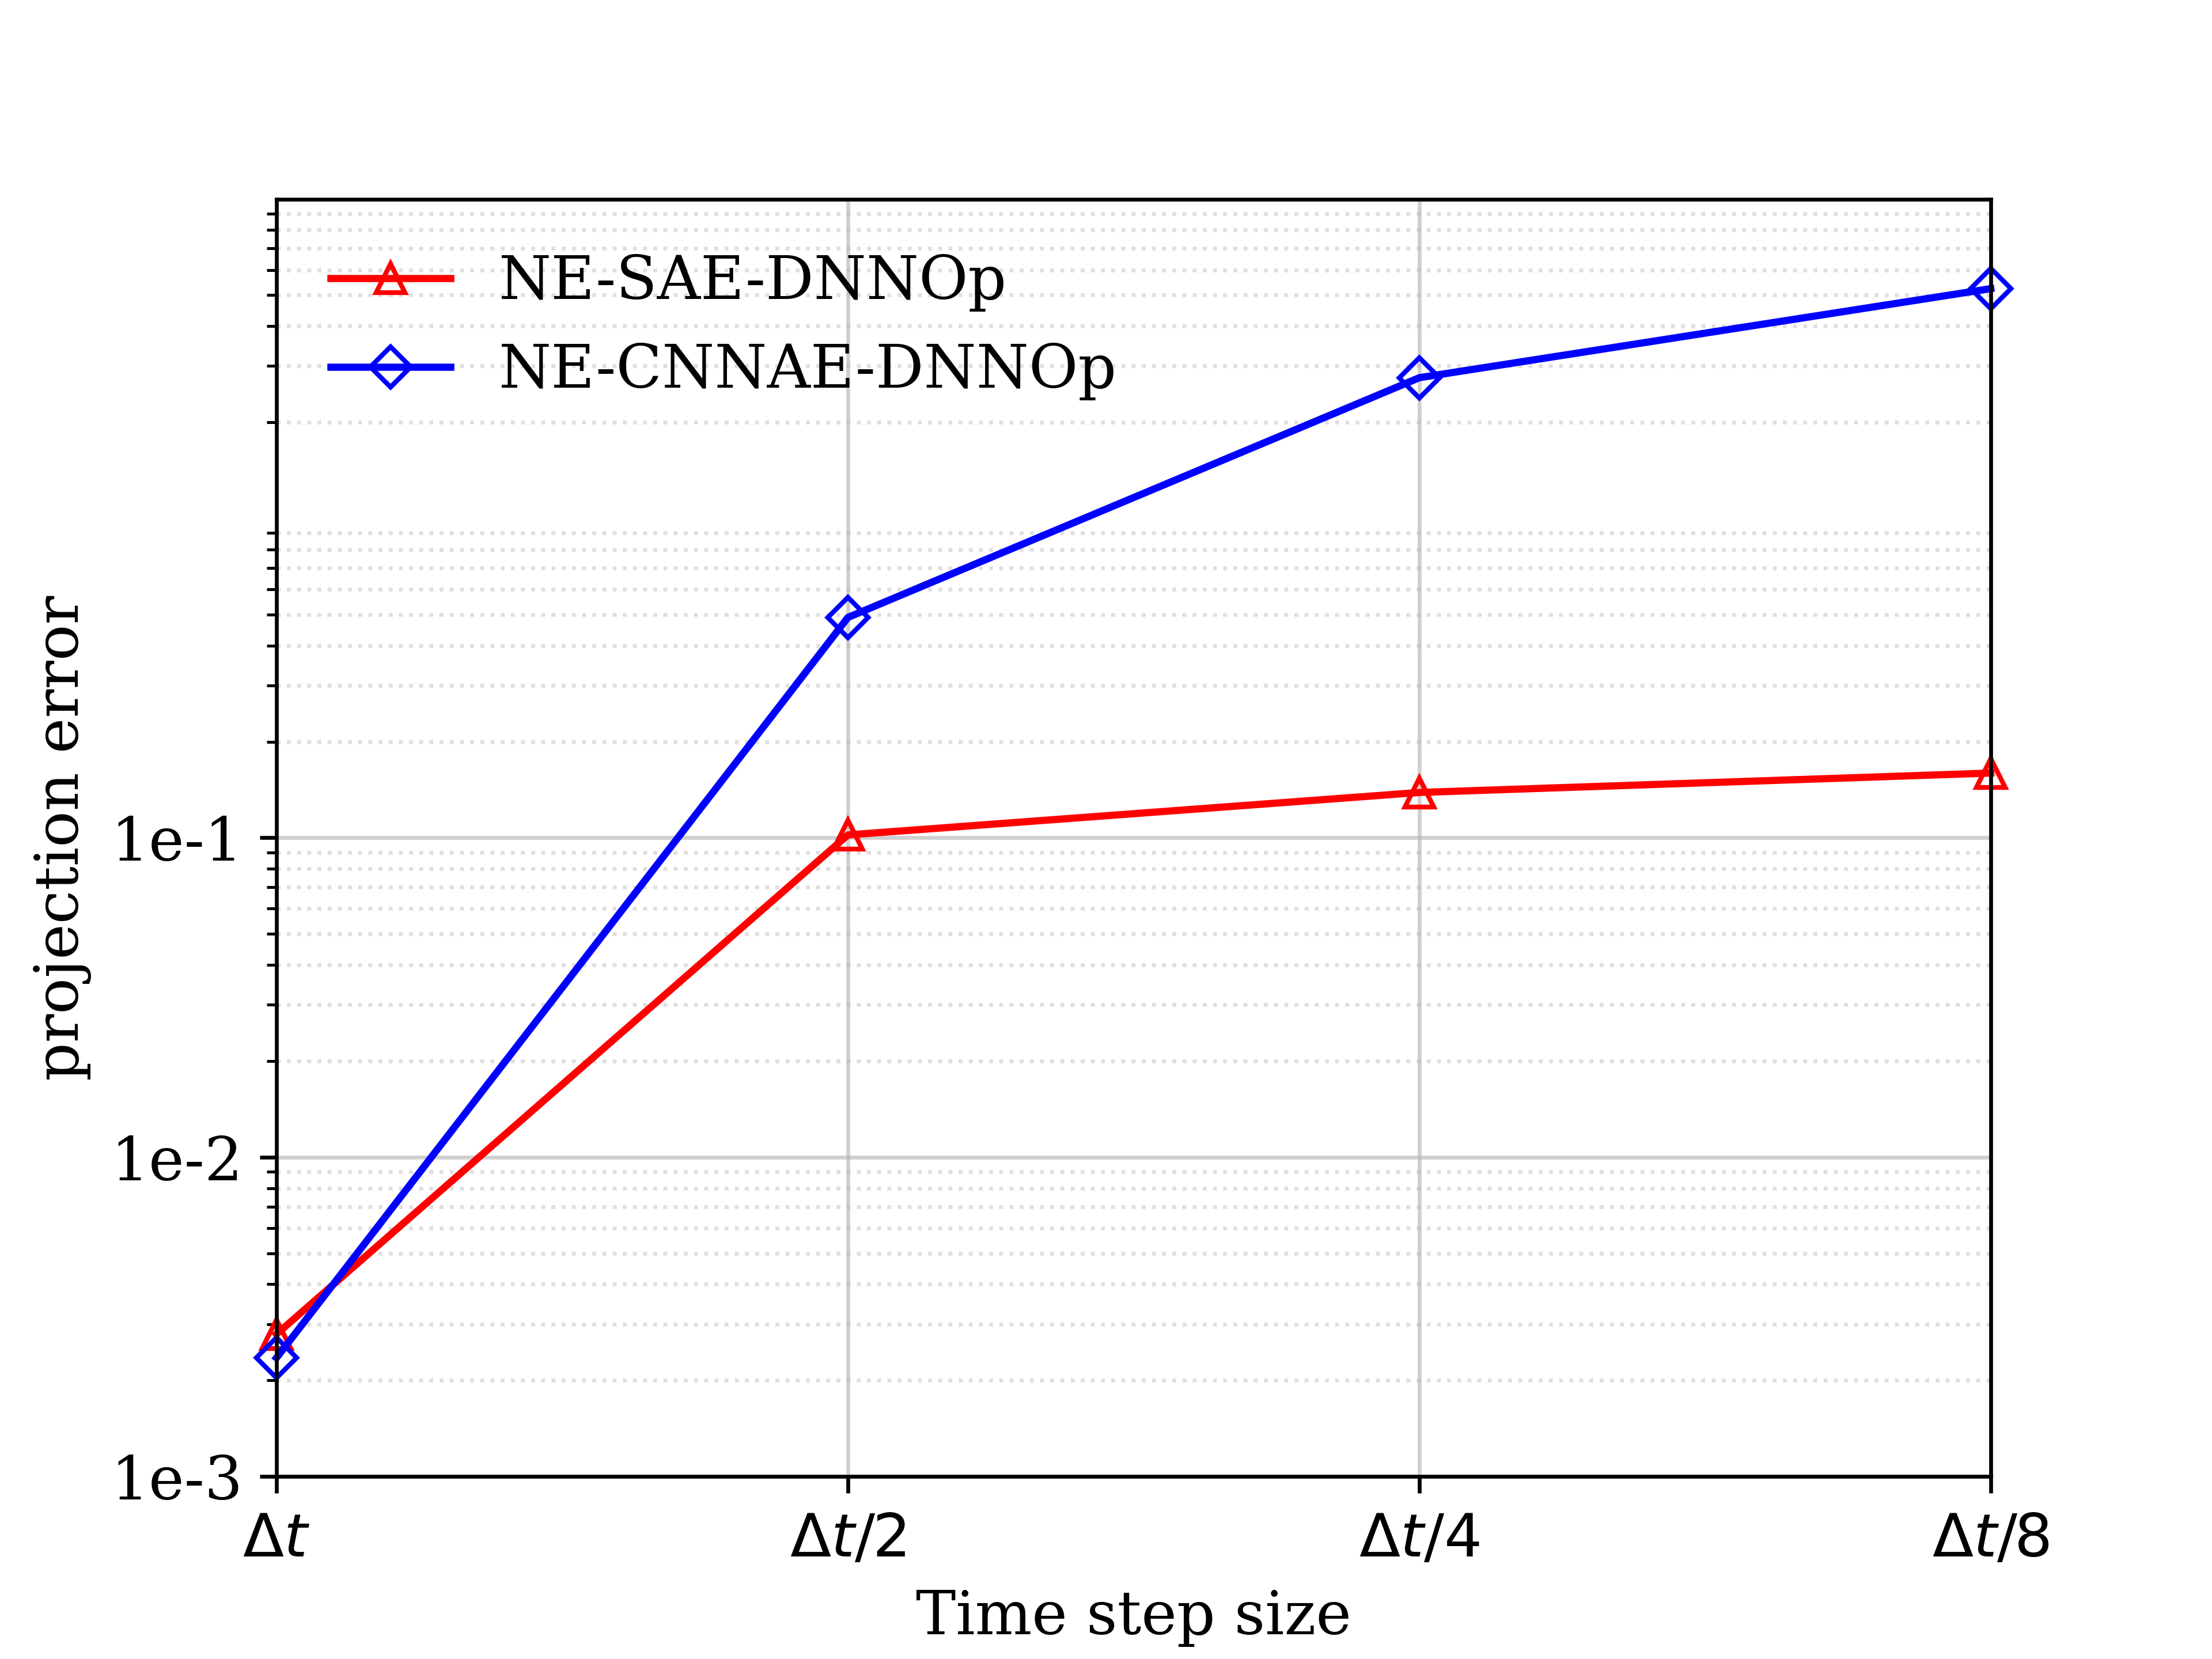
\includegraphics[width=\textwidth]{rom_time_step_size.png}
            \end{center}
            \caption{}
        \end{subfigure}
     \end{center}
        \caption[Time step-size dependency.]{(a) Projection error of the solution in the latent space; and (b) projection error of the reduced-order model  with $r = 20$ on the test dataset over different time step sizes. Here, $\Delta t$ is the time step size used for training the autoencoders and the reduced operators.}
        \label{fig: time step size dependency}
\end{figure}
It is seen that both errors substantially increase as the time resolution is refined, which is consistent with results reported elsewhere (see, e.g., \cite{ZHU2018415} for similar behavior with space discretization). The increase in the ROM projection error is larger for CNNAE than for SAE (see the right panel in Fig.~\ref{fig: time step size dependency}), which may be attributed to the fact that the adaptive basis is constructed for a given time step size.